\documentclass[fleqn,usenatbib]{mnras}
%
%\hypersetup{draft}  %%% only for draft

%\usepackage{natbib}
\usepackage{xr-hyper}

%from mnras:
\usepackage{hyperref}	% Hyperlinks
\hypersetup{colorlinks=true,linkcolor=blue,citecolor=blue,filecolor=blue,urlcolor=blue}

\usepackage[russian]{babel}
\usepackage[utf8]{inputenc}

\usepackage{mathptmx}
\usepackage[T1]{fontenc}
\usepackage{ae,aecompl}
\usepackage{graphicx}	% Including figure files
\usepackage{amsmath}	% Advanced maths commands
\usepackage{amssymb}	% Extra maths symbols
\usepackage{multicol}   % Multi-column entries in tables
\usepackage{bm}         % Bold maths symbols, including upright Greek
\usepackage{pdflscape}  % Landscape pages
\usepackage{enumitem}
\usepackage{xspace}
\usepackage{hhline}
\def\beq#1{\begin{equation}\label{#1}}
\def\eeq{\end{equation}}

\usepackage{comment}

% for referecnes in tables
\usepackage{array}
\usepackage{etoolbox}
\usepackage{multirow}

\usepackage{color}
\newcommand{\achtung}[1]{\textcolor{red}{//#1//}}
\newcommand{\mesch}[1]{\textcolor{orange}{//#1//}}
\newcommand{\tibercus}[1]{\textcolor{teal}{//#1//}}

% for newpage
% \usepackage{titlesec}
% \newcommand{\sectionbreak}{\newpage}
% \newcommand{\subsectionbreak}{\newpage}

\title[SRGz: photo-z predictions]{SRGz: photo-z predictions for point X-ray sources}
\author[Borisov et al.]{Victor Borisov, Alexander Meshcheryakov %\newauthor 
}
\date{September 2020}

%%%%%%%%%%%%%%%%%%%%
%DO NOT CHANGE
\makeatletter
\newcommand*{\addFileDependency}[1]{% argument=file name and extension
  \typeout{(#1)}
  \@addtofilelist{#1}
  \IfFileExists{#1}{}{\typeout{No file #1.}}
}
\makeatother

\newcommand*{\myexternaldocument}[1]{%
    \externaldocument{#1}%
    \addFileDependency{#1.tex}%
    \addFileDependency{#1.aux}%
}
%%%%%%%%%%%%%%%%%%%%
%CHANGE
%\myexternaldocument{pdf_figures}
%%%%%%%%%%%%%%%%%%%

\usepackage{pdflscape}
\begin{document}

% for references in tables
\newcounter{rowcntr}[table]
\renewcommand{\therowcntr}{\arabic{rowcntr}}
% A new columntype to apply automatic stepping
\newcolumntype{N}{>{\refstepcounter{rowcntr}\therowcntr}c}
% Reset the rowcntr counter at each new tabular
\AtBeginEnvironment{tabular}{\setcounter{rowcntr}{0}}

\newcommand{\expnumber}[2]{{#1}\mathrm{e}{#2}}

\maketitle
\begin{abstract}
Проведено исследование, построение и сравнение моделей вероятностных прогнозов фотометрических красных смещений (photo-z) на основе алгоритма случайного леса  с использованием данных современных астрономических обзоров SDSS, PanStarrs и DESI Legacy Survey для построения трехмерной карты квазаров.

Предложена модель photo-z, значительно превосходящая (в ~2 раза) по точности (метрики точечных прогнозов — нормализованное медианное абсолютное отклонение NMAD и доля выбросов n>0.15) лучшие модели (SOTA) известные в литературе. Для рентгеновских источников в тестовой области неба Stripe82X получена точность NMAD = 0.034 / 0.064 / 0.067 и n>0.15 = 0.079 / 0.170 / 0.163 для предложенной модели / шаблонной модели Ananna, 2017 / нейросетевой модели Brescia, 2019, соответственно.
\end{abstract}

% ===============================================================================
% ===============================================================================
% ===============================================================================


\section{Inctoduction}

On July 13, 2019 the SRG X-ray observatory
was launched from the Baikonur cosmodrome. On Dec. 8th, 2019 SRG started its first All-Sky Survey, which will consist of 8 repeated six month long scans of the entire sky. eROSITA telescope \citep{2020arXiv201003477P} onboard SRG operates in the soft X-ray band (0.3–8\,keV) and will detect $\sim3$ millions X-ray AGNs at the end of survey. In order to construct a large-scale structure map of X-ray Universe with eROSITA, accurate measurements of cosmological redshifts for extragalactic X-ray sources (mostly quasars) are needed.

Redshift measurement methods \citep{2019NatAs...3..212S} can be divided into spectroscopic (spec-z, $z_{sp}$) and photometric (photo-z, $\hat{z}_{ph}$). Spec-z's are time consuming task for faint optical objects ($r\gtrsim22^{mag}$). On the other hand, photo-z measurements can be based on data from modern large photometric sky surveys, it is much cheaper in observational resources than spec-z but also less accurate. 

В задаче измерения photo-z возникает проблема мультимодальности прогнозов. На рисунке (тут нужен хороший рисунок с примерами двух спектров и прогнозами) представлен пример спектров двух галактик, находящихся на разном красном смещении. Видно, что в некотором диапазоне излучения их спектры сильно похожи, и, как следствие, сильно похожи фотометрические признаки (отмечены черными точками на графике). Таким образом получается неоднозначное соответствие прогнозов признакам, и точечная оценка, построенная на основе этих признаков, скорее всего, будет неверной. Поэтому необходимо прогнозировать не само значение красного смещения объекта, а распределение значения красного смещения объекта. Такой прогноз называется вероятностным фотометрическим красным смещением (вероятностный photo-z). Вероятностный photo-z позволит вычислять доверительные интервалы, оценивать надежность прогнозов.

In this work we present machine learning models for X-ray sources probabilistic photo-z predictions, based on photometric data from 4 modern sky surveys (SDSS, Pan-STARRS1, DESI Legacy Imaging Survey, and WISE).

\subsection{Related works}
Общие подходы к решению задачи прогноза photo-z описываются в \cite{bib:nature_photoz}. Все решения, предлагаемые для решения данной задачи можно разделить на 2 группы: основанные на использовании физических моделей (Physically motivated methods, шаблонные модели) и основанные на использовании данных (Data driven methods), т.е. с применением технологий машинного обучения.

Суть методов на основе шаблонов состоит в использовании спектров типовых объектов различных классов. На основе спектра строится шаблон -- физическая модель предсказывающая значение фотометрических признаков по значению красного смещения, составляется библиотека шаблонов. Далее производится поиск оптимального шаблона, на котором достигается минимальная ошибка между предсказанными фотометрическими признаками и измеренными, путем минимизации критерия \(\mathcal{X}^2\)
\begin{equation}
    \mathcal{X}^2 (z, T, A) = \sum_i^{N_{filters}} (\frac{F_{obs}^i - A~F_{pred}^i(T, z)}{\sigma_{obs}^i})^2,
\end{equation}
где \(z\) -- значение красного смещения, \(N_{filetrs}\) -- количество фильтров (фотометрических признаков), \(F_{obs}^i\) и \(\sigma_{obs}^i\) -- наблюдаемое значение \(i\)-ого признака и ошибка на него, \(F_{pred}^i(T, z)\) -- значение \(i\)-ого признака, полученное из шаблона \(T\) для красного смещения \(z\), \(A\) -- фактор нормализации. Таким образом определяется не только красное смещение объекта, но и его тип.

Такие модели представлены в пакетах ...

Однако, такие методы показывают точность хуже методов машинного обучения при наличии большой репрезентативной обучающей выборки. Основные алгоритмы, применяемые для прогнозов фотометрических красных смещений -- искусственные нейронные сети, ближайшие соседи и методы на основе ансамблей деревьев решений, которые показывают лучшую точность в данной задаче.

В пакете ANNz2 \cite{bib:annz2} реализованы методы на основе многослойного персептрона, деревьев бустинга (boosted decision trees) и регрессии k-ближайших соседей. Реализованные в пакете алгоритмы позволяют оценивать достоверность прогноза, и в качестве финального прогноза дается лучший из прогнозов ансамбля моделей или взвешенная сумма прогнозов. В сравнении использовался ансамбль из пяти многослойных персептронов с архитектурой слоёв 6:12:12:1, где на вход подавались данные шести фильтров ugrizy и на выходном слое получается прогноз photo-z. Каждый персептрон обучался со случайной инициализацией параметров.

В пакете CMNN \cite{bib:cmnn} для прогноза photo-z используется метод ближайших соседей. В качестве признаков выступают, так называемые цвета (отношение яркостей между разными фильтрами), расстоянием между соседями выступает расстояние Махалонобиса
\begin{equation}
    D_M = \sum_j^{N_{colors}} \frac{(c_{j,train} - c_{j,test})^2}{(\delta c_{j,test})^2},
\end{equation}
и в качестве прогноза дается взвешенная сумма целевых признаков соседей с весами, обратными расстояниям до них.
%\achtung{пока не очень въехал в описание. Дописать}

FlexZBoost \cite{bib:flexzboost} представляет собой набор общих методов адаптации алгоритмов оценки условного среднего для оценки условной плотности распределения целевого признака. Для этого неизвестная функция плотности раскладывается по ортонормированному базису. В статье было использовано преобразование Фурье. Далее коэффициенты Фурье вычисляются как точечная оценка с использованием выбранного алгоритма машинного обучения (в статье использовался xgboost).

Алгоритм GPz \cite{bib:gpz} основан на использовании гауссовых процессов. 

METAPhoR \cite{bib:metaphor} представляет собой алгоритм вероятностных прогнозов photo-z, позволяющий адаптировать алгоритмы регрессии для получения вероятностных оценок. По умолчанию используется многослойный персептрон обучение которого происходит квазиньютоновским алгоритмом (Multi Layer Perceptron with Quasi Newton Algorithm, MLPQNA) минимизацией ошибки MSE с применением L2-регуляризации. Для получения вероятностного прогноза признаки объекта разыгрываются в соответствии с ошибками измерений на них. Модели, реализованные в данном пакете были применены в статье Brescia для прогноза photo-z рентгеновских источников.

В пакете SkyNet \cite{bib:skynet} используются многослойный персептрон, обучаемый методом градиентного спуска второго порядка минимизацией кросс-энтропийной функции потерь, то есть решается задача классификации. Область определения целевого признака разбивается на 200 интервалов, объект принадлежит к некоторому классу, если его целевой признак принадлежит к соответствующему интервалу. Вероятностный прогноз получается из двухсот выходов выходного слоя с функцией активации softmax нейронной сети, на вход алгоритма подаются измерения и ошибки измерения шести фотометрических признаков (всего 12 входов).

В TPZ \cite{bib:tpz} используется алгоритм случайного леса без ограничения глубины. Вероятностный прогноз получается путем решения множества задач бинарной классификации: область определения целевого признака разбивается на интервалы, и для каждого интервала строится модель классификации, которая определяет, принадлежит ли значение целевого признака заданному интервалу или не принадлежит. Вероятностный прогноз представляет собой набор вероятностей принадлежности значения целевого признака тому или иному интервалу.

В \cite{bib:mesch} были предложены методы, основанные на использовании случайного леса и квантильного градиентного бустинга, для получения вероятностных прогнозов фотометрических красных смещений.

Метод, основанный на алгоритме случайного леса, заключается в получении прогноза распределения в виде независимой выборки точечных прогнозов деревьев, построенных без ограничения глубины. Независимость достигается за счет того, что деревья в методе случайного леса строятся независимо на случайных подвыборках обучающей выборки. Далее для оценки непрерывной функции плотности вероятности (для получения вероятностного прогноза) используется ядерная оценка плотности.

Метод квантильного градиентного бустинга заключается в обучении модели с квантильной функцией потерь, которую для фиксированного значения \(\alpha \in [0,1]\) можно записать следующим образом
\begin{equation}
    l(y_i, \hat{y}_{\alpha, i}) = (1-\alpha)|y_i - \hat{y}_{\alpha, i}|\mathbb{I}[y \leq \hat{y}_{\alpha, i}] + \alpha|y_i - \hat{y}_{\alpha, i}|\mathbb{I}[y > \hat{y}_{\alpha, i}],
\end{equation}
где \(y_i\) - истинное значение, \(\hat{y}_{\alpha, i}\) - предсказанное значений целевой переменной. Таким образом, вероятностный прогноз, являющийся результатом работы этого алгоритма будет представлен ансамблем заданных квантилей. Стоит заметить, что в методе градиентного бустинга каждое следующее дерево строится для антиградиента предыдущего, что делает их не независимыми, и делает невозможным получение вероятностного прогноза в представлении выборки независимых значений, как это реализовано в случайном лесе.

\subsection{Цели работы и структура статьи}
In this paper we present photo-z models based on various photometric data, thus having different area of usage in terms of sky coverage. We analyse models quality depending on observed values (magnitude, photo-z prediction) and spectral redshift (target value). The structure of this work is as follows.

In section \ref{sec:data} we describe data we use: photometry, spectral data, train and test samples assembling, and models we present (because, our models are primarily defined by photometry they use).

In section \ref{sec:thealgorithm} we describe probabilistic regression problem and machine learning algorithm solving this problem we use to construct photo-z models.

In section \ref{sec:results} we describe the way we present our results, quality metrics of photo-z predictions and present results themselves.

In section \ref{sec:conclusion} we outline the main results of this work.

% ===============================================================================
% ================================ Data =========================================
% ===============================================================================

\section{Data}\label{sec:data}
\subsection{Photometric data}
We use photometric data from SDSS DR14 \citep{2018ApJS..235...42A}, Pan-STARRS1 DR2 \citep{2018AAS...23110201C}, DESI LIS DR8 \citep{2019AJ....157..168D} sky surveys and WISE forced photometry \citep{2010AJ....140.1868W}. A brief description of each of the sky surveys is given in Table \ref{tab:catalogs_comparison}.

It is important to note that only Pan-STARRS covers the entire eastern hemisphere of the sky, so photo-z models based only on Pan-STARRS data are of particular interest to the Russian eRosita consortium.

\begin{table*}
    \caption{Comparison of photometric sky surveys from which photometric data were used by the presence of filters and the coverage area of the sky.}
    \label{tab:catalogs_comparison}
    \centering
    \begin{tabular}{|l|c|c|c|c|}
    \hline
        Survey & Filters & Types of fluxes & Sky coverage (sq.degrees) & Ref \\
    \hline
        SDSS DR16 & u,g,r,i,z & PSF, cModel & 14555 (1/3 of the sky) & Ref\\
        Pan-STARRS1 DR2 & g,r,i,z,y & PSF, Kron & 30000 (3/4 of the sky) & \\
        DESI LIS DR8 & g,r,z & Model & 14000 (1/3 of the sky) & \\
        WISE & w1,w2,w3,w4 & forced photometry & whole sky & \\[1ex]
        \hline
    \end{tabular}
\end{table*}

\begin{figure*}
    \centering
    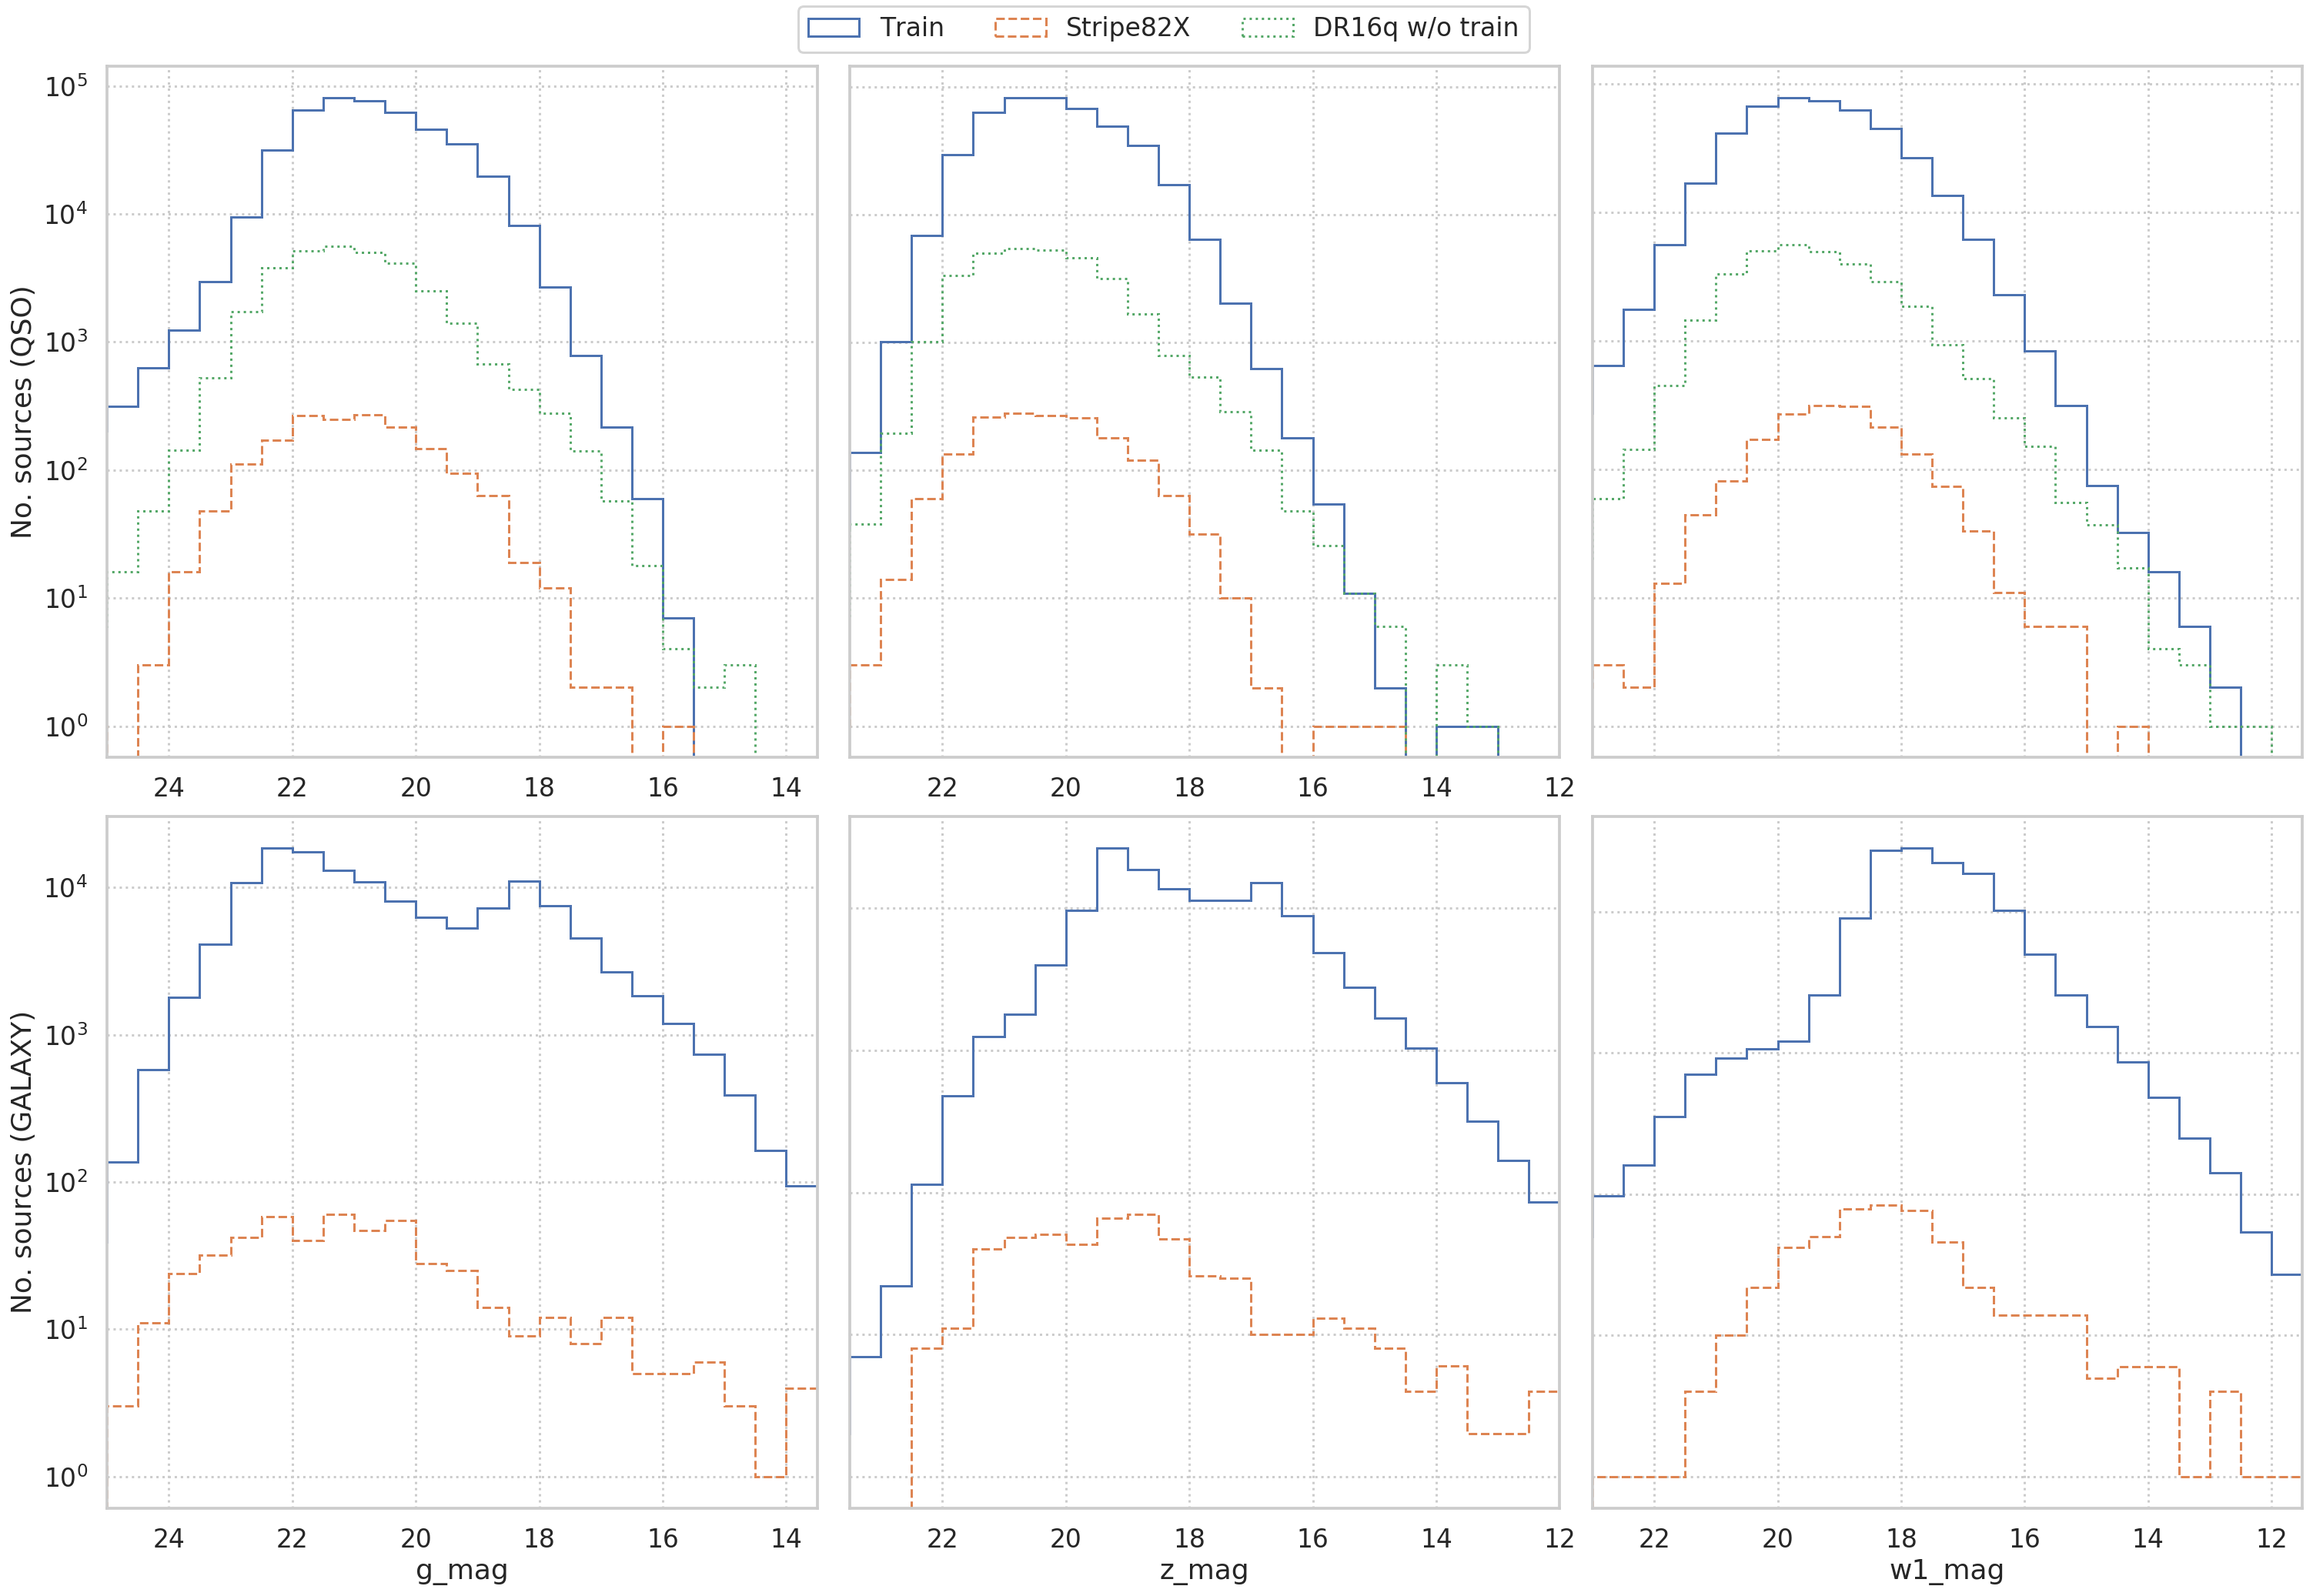
\includegraphics[width=0.9\linewidth]{images/data-dist-mags-ab_final.png}
    \caption{Histograms of object distributions in the samples according to the magnitude value of \eqref{eq:mag_ab} in the blue (g), red (z), and infrared (w1) filters. The first line of the graphs is the distribution of the training sample, the second line of the graphs is the distribution of the Stripe82X sample, and the third line is the distribution of the test sample of the SDSS DR16q quasars. The blue solid line shows the distribution of quasars, and the orange line shows the distribution of galaxies.}
    \label{fig:data-dist-mags-ab}
\end{figure*}

\begin{figure*}
    \centering
    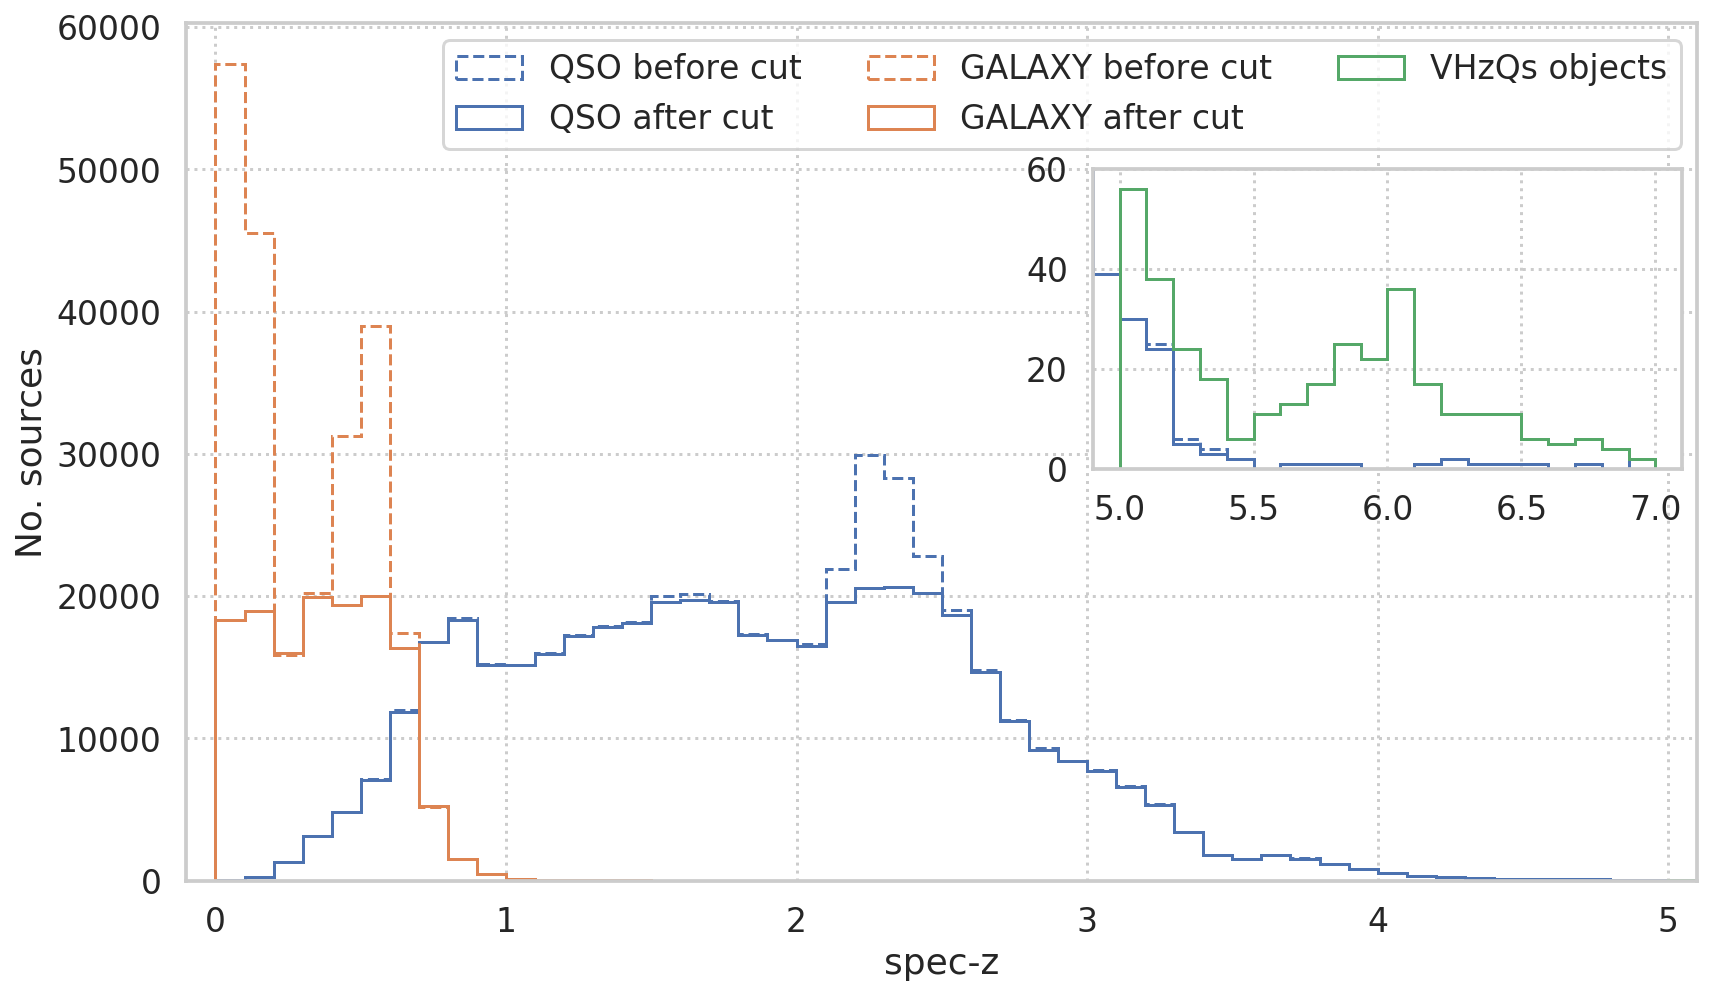
\includegraphics[width=0.95\linewidth]{images/train-peaks-cut.png}
    \caption{Pre-processing of the training sample. The histogram of the distribution of the SDSS DR14 galaxies included in the sample is shown in orange, the SDSS DR14q quasars are shown in blue, and the VHzQs quasars are shown in green. The dashed lines are the distributions before the alignment, and the solid lines are the distributions after the alignment.}
    \label{fig:train-peaks-cut}
\end{figure*}

\begin{figure}
    \centering
    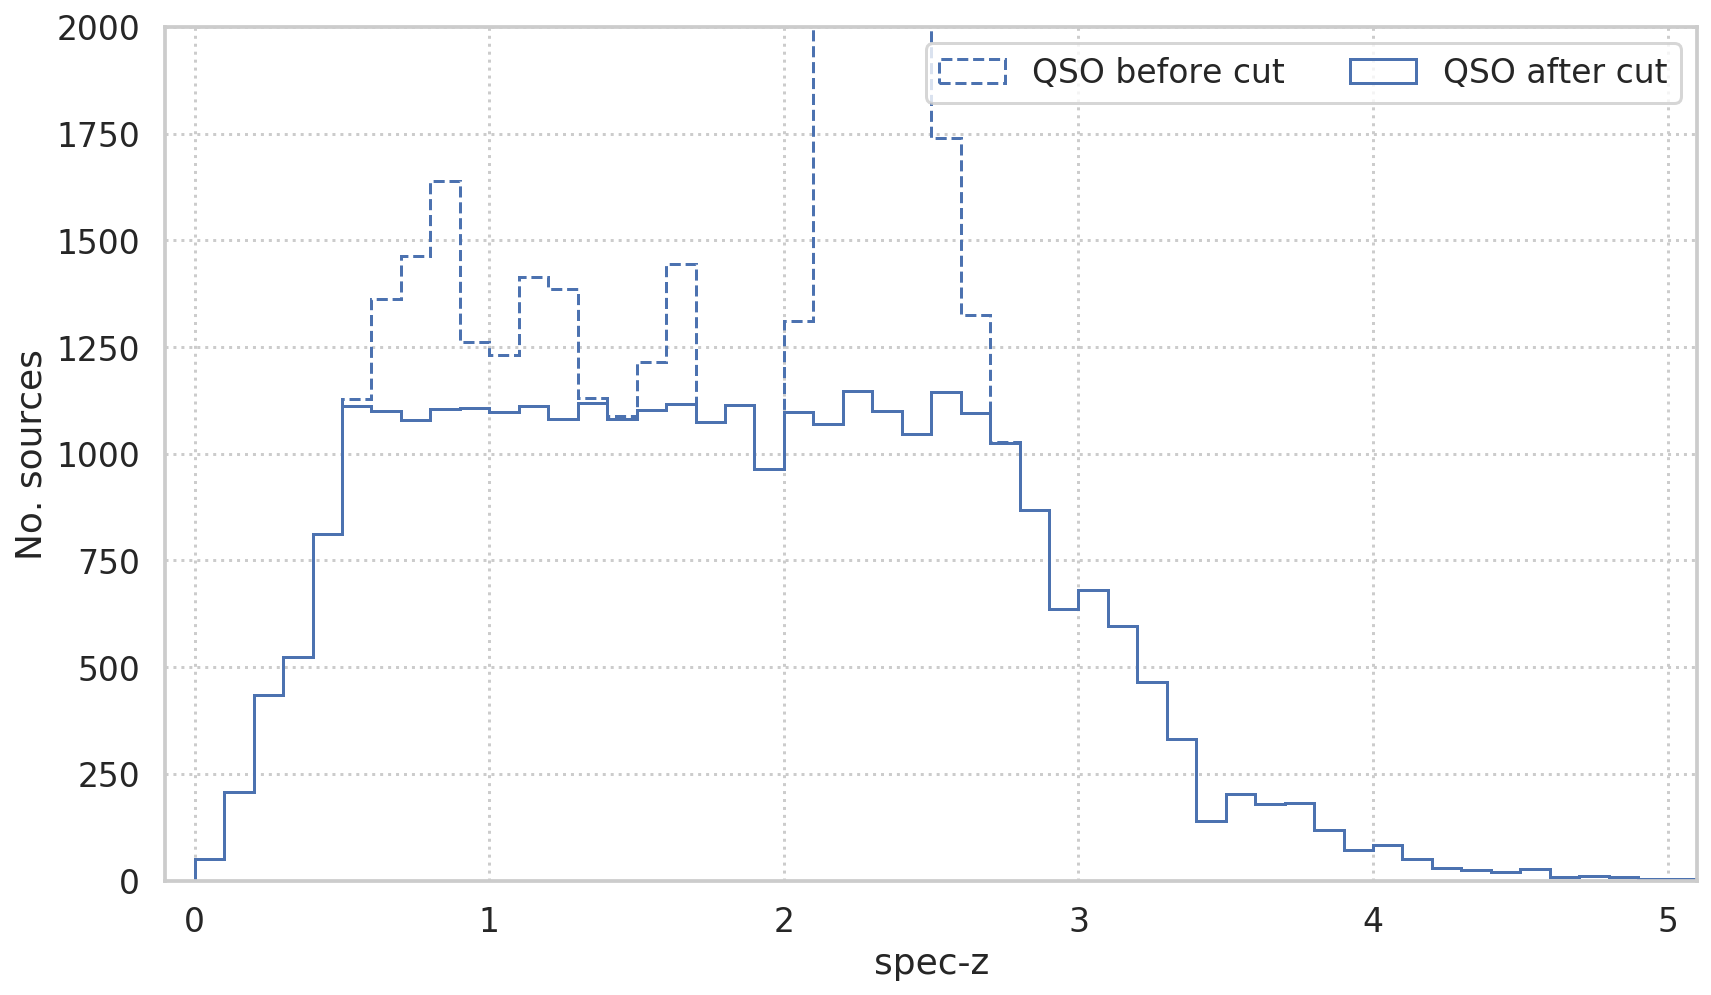
\includegraphics[width=0.95\linewidth]{images/data-dist-dr16q-peaks-cut.png}
    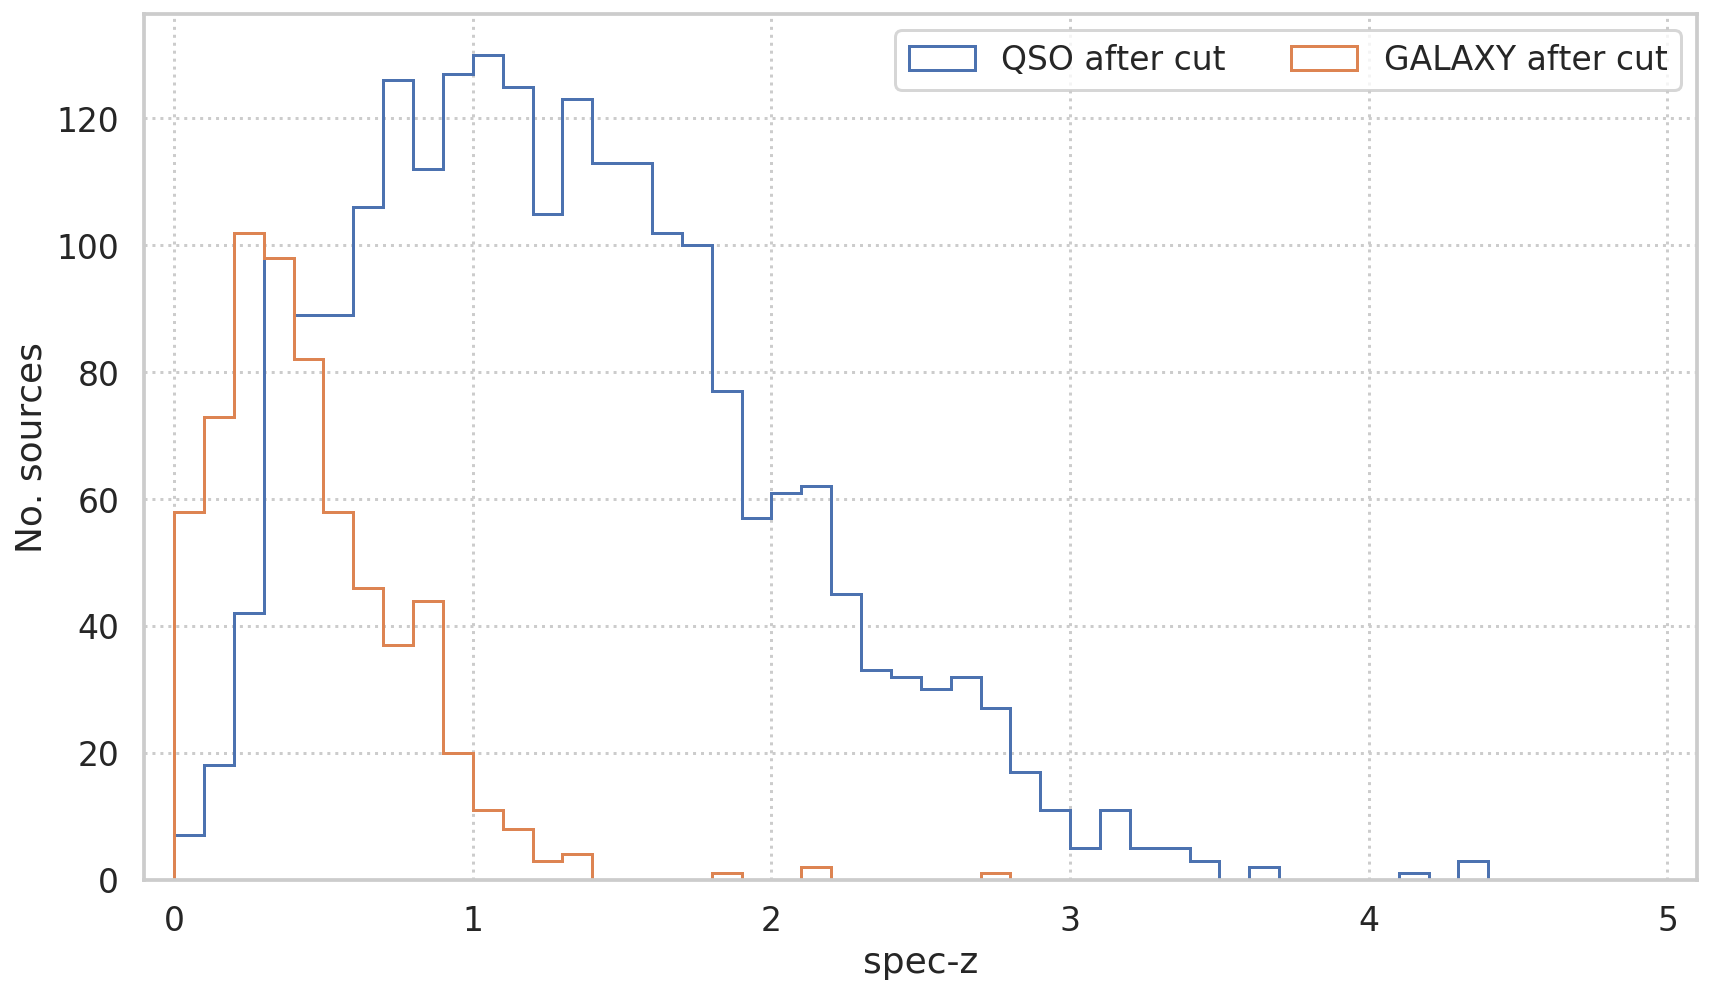
\includegraphics[width=0.95\linewidth]{images/data-dist-s82x.png}
    \caption{Spec-z distribution for DR16q (top) and S82X (bottom panel) test samples.}
    \label{fig:dr16q-peaks-cut}
\end{figure}

%\begin{figure}
%    \centering
%    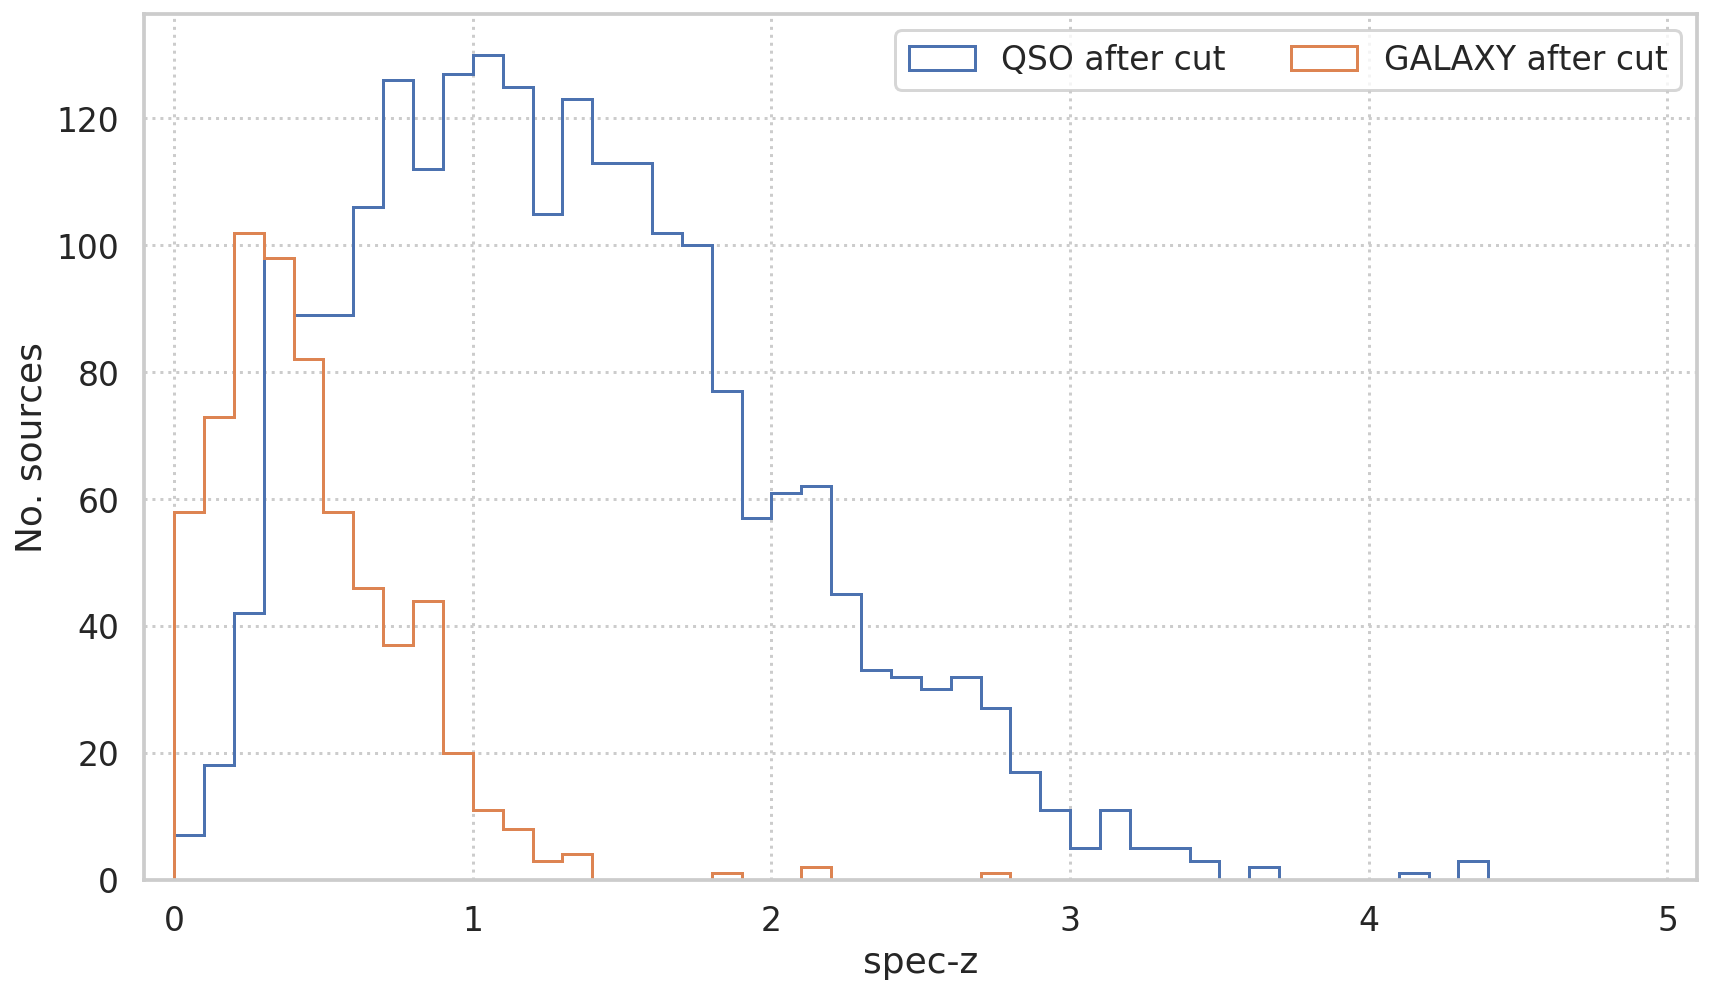
\includegraphics[width=0.95\linewidth]{images/data-dist-s82x.png}
%    \caption{S82X}
%    \label{fig:data-dist-s82x}
%\end{figure}

\subsection{Main spectral sample}

The SDSS spectral catalog was used to compile a large training sample (see Table \ref{tab:samples}). Optical galaxies SDSS DR14 and quasars SDSS DR14q Paris'18 were balanced by class in order to approximate the distribution of X-ray sources. The distribution of the training sample objects was then aligned as shown in Figure 1. and the VHzQs quasars (Ross \& Corss, 20??) were added. The properties of the sample are shown in more detail in Figures \ref{fig:data_distribution} and \ref{fig:data-dist-mags-ab}.

\subsection{DR16q quasars test sample}
For a more detailed analysis of the behavior of the models on objects with $spec-z > 3$, a test sample of quasars was compiled. The objects with the most reliably measured spectral redshifts (\texttt{Z\_CONF == 3 and SOURCEZ == VI}) were selected from the SDSS DR16q spectral catalog, and the distribution peak at $z \sim 3$ was cut off, similarly to the training sample. The properties of the sample are shown in more detail in Figures \ref{fig:data_distribution} and \ref{fig:data-dist-mags-ab}.

\subsection{Stripe82X test sample}
The Stripe82X sample of X-ray objects was first presented in (Ananna, 2017). This sample is currently the largest sample of X-ray objects with a qualitative classification by spectra, and it is marked by hand, which makes it the main test sample for the comparison of photo-z X-ray object models. The results chapter will compare our models with State-Of-The-Art models: the template model (Ananna, 2017) and the neural network model (Brescia, 2019). The properties of the sample are shown in more detail in Figures \ref{fig:data_distribution} and \ref{fig:data-dist-mags-ab}.

\begin{table*}
	\begin{tabular}{lllllllll}
            \hline
            {} & \multicolumn{3}{l}{No. sources} & \multicolumn{5}{l}{With photometry from} \\
            Sample &       Total &  Galaxy &     QSO &                   LS &      PS & LS \& PS & SDSS \& PS & All 3 surveys \\
            \hline
            Train sample                                              &      586176 &  136428 &  449748 &               580511 &  582240 &   579329 &     578815 &        577049 \\
            Stripe82X                                                 &        2653 &     508 &    1701 &                 2643 &    2224 &     2200 &       2224 &          2200 \\
            S82X ($\expnumber{3}{-15} <= FSoft < \expnumber{1}{-14}$) &        1152 &     297 &     656 &                 1147 &     935 &      922 &        935 &           922 \\
            S82X ($\expnumber{1}{-14} <= FSoft < \expnumber{4}{-14}$) &        1259 &     194 &     859 &                 1256 &    1078 &     1069 &       1078 &          1069 \\
            S82X ($FSoft > \expnumber{4}{-14}$)                       &         242 &      17 &     186 &                  240 &     211 &      209 &        211 &           209 \\
            DR16q w/o train test                                      &       31867 &       0 &   31867 &                31750 &   27203 &    27156 &      27203 &         27156 \\
            \hline
            \end{tabular}
            \caption{Description of the samples used. The first column gives the name of the sample, the next three columns are the number of objects (total, separate galaxies, separate quasars), the next five columns are the number of objects with full DESI LIS photometry, Pan-STARRS, DESI LIS and Pan-STARRS simultaneously, SDSS and Pan-STARRS simultaneously, and all three surveys simultaneously, respectively. <<LS>> stands for DESI LIS, and <<PS>> stands for Pan-STARRS.}
\end{table*}


\begin{figure*}
    \centering
    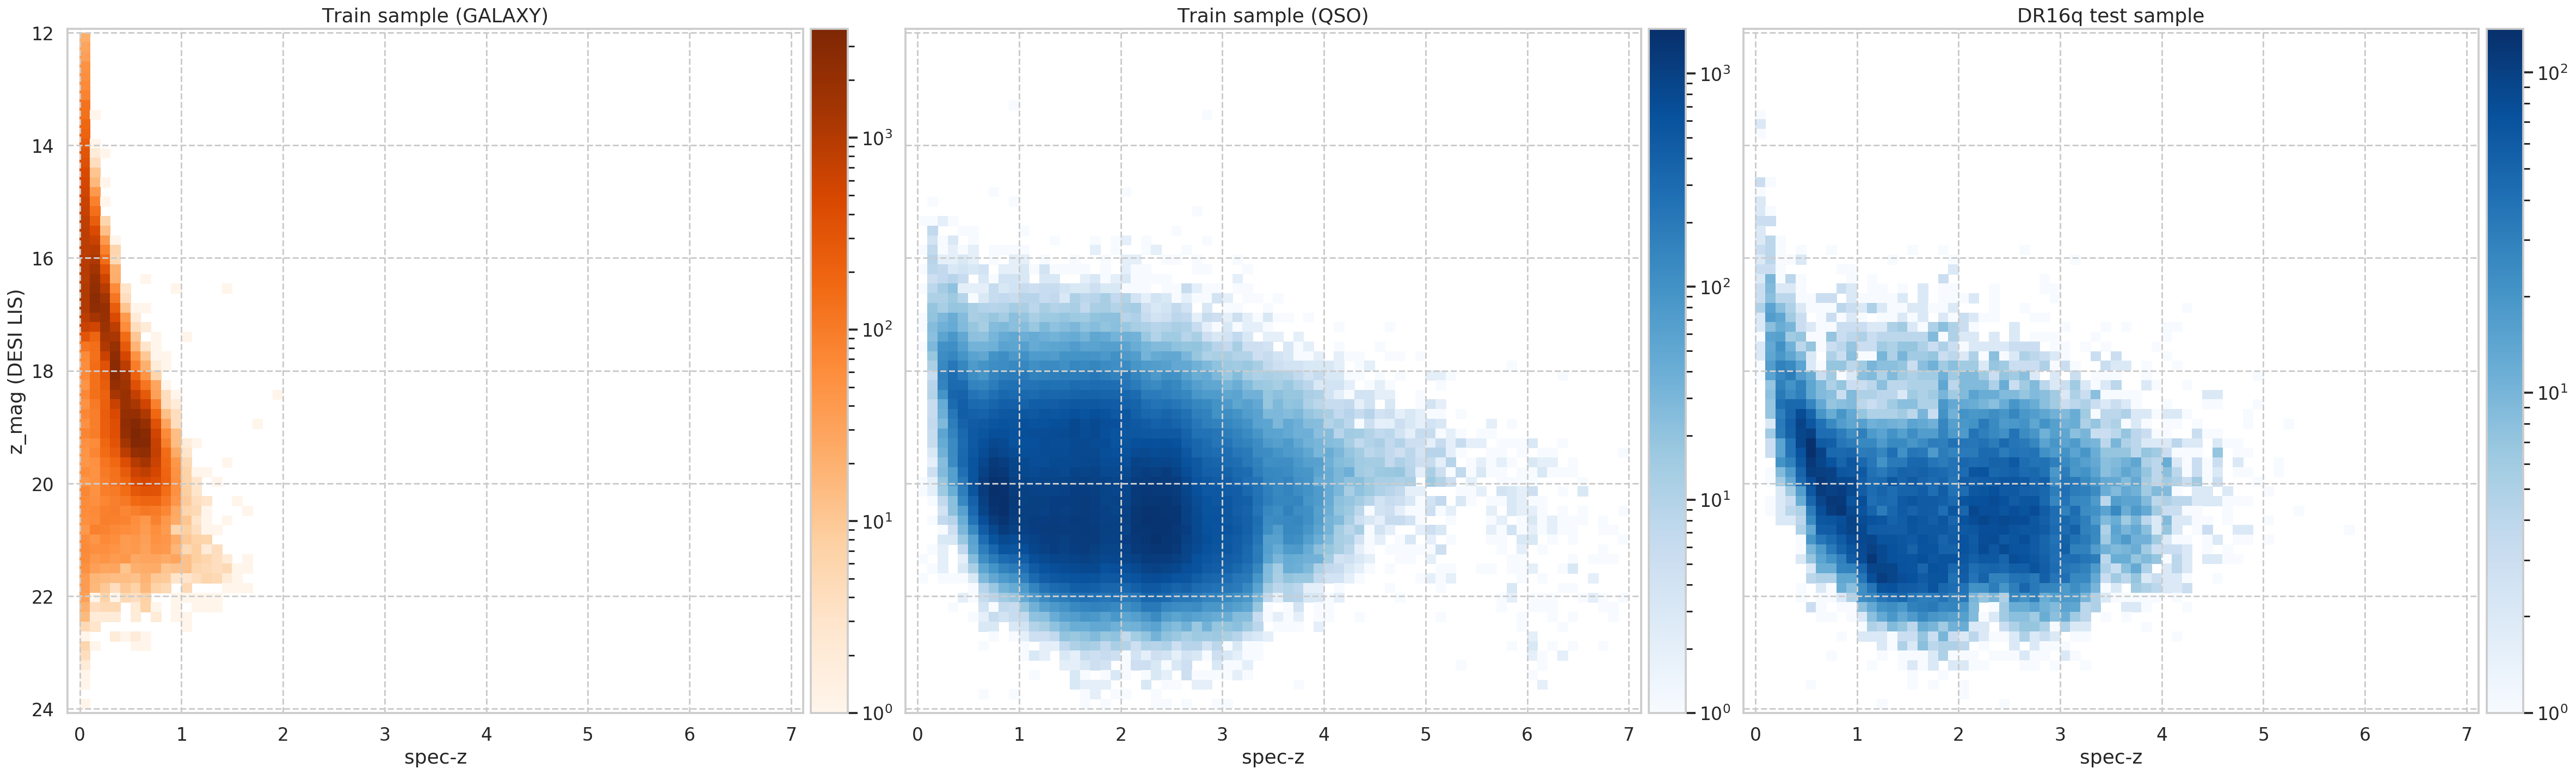
\includegraphics[width=0.95\linewidth]{images/data-dist-ab-upsidedown-dr16.png}
    \caption{The distributions of the objects in the used samples. The abscissa axis is the spectral redshift, the ordinate axis is the value \eqref{eq:mag_ab} in the $z$ filter. The upper line of the graphs, from left to right, is the distributions of galaxies and quasars in the training sample and the test sample of SDSS DR16q quasars.  The bottom line of the graphs is the distribution of Stripe82X objects with different X-ray fluxes. Orange circles show galaxies, blue crosses show quasars.}
    \label{fig:data_distribution}
\end{figure*}

\begin{figure*}
    \centering
    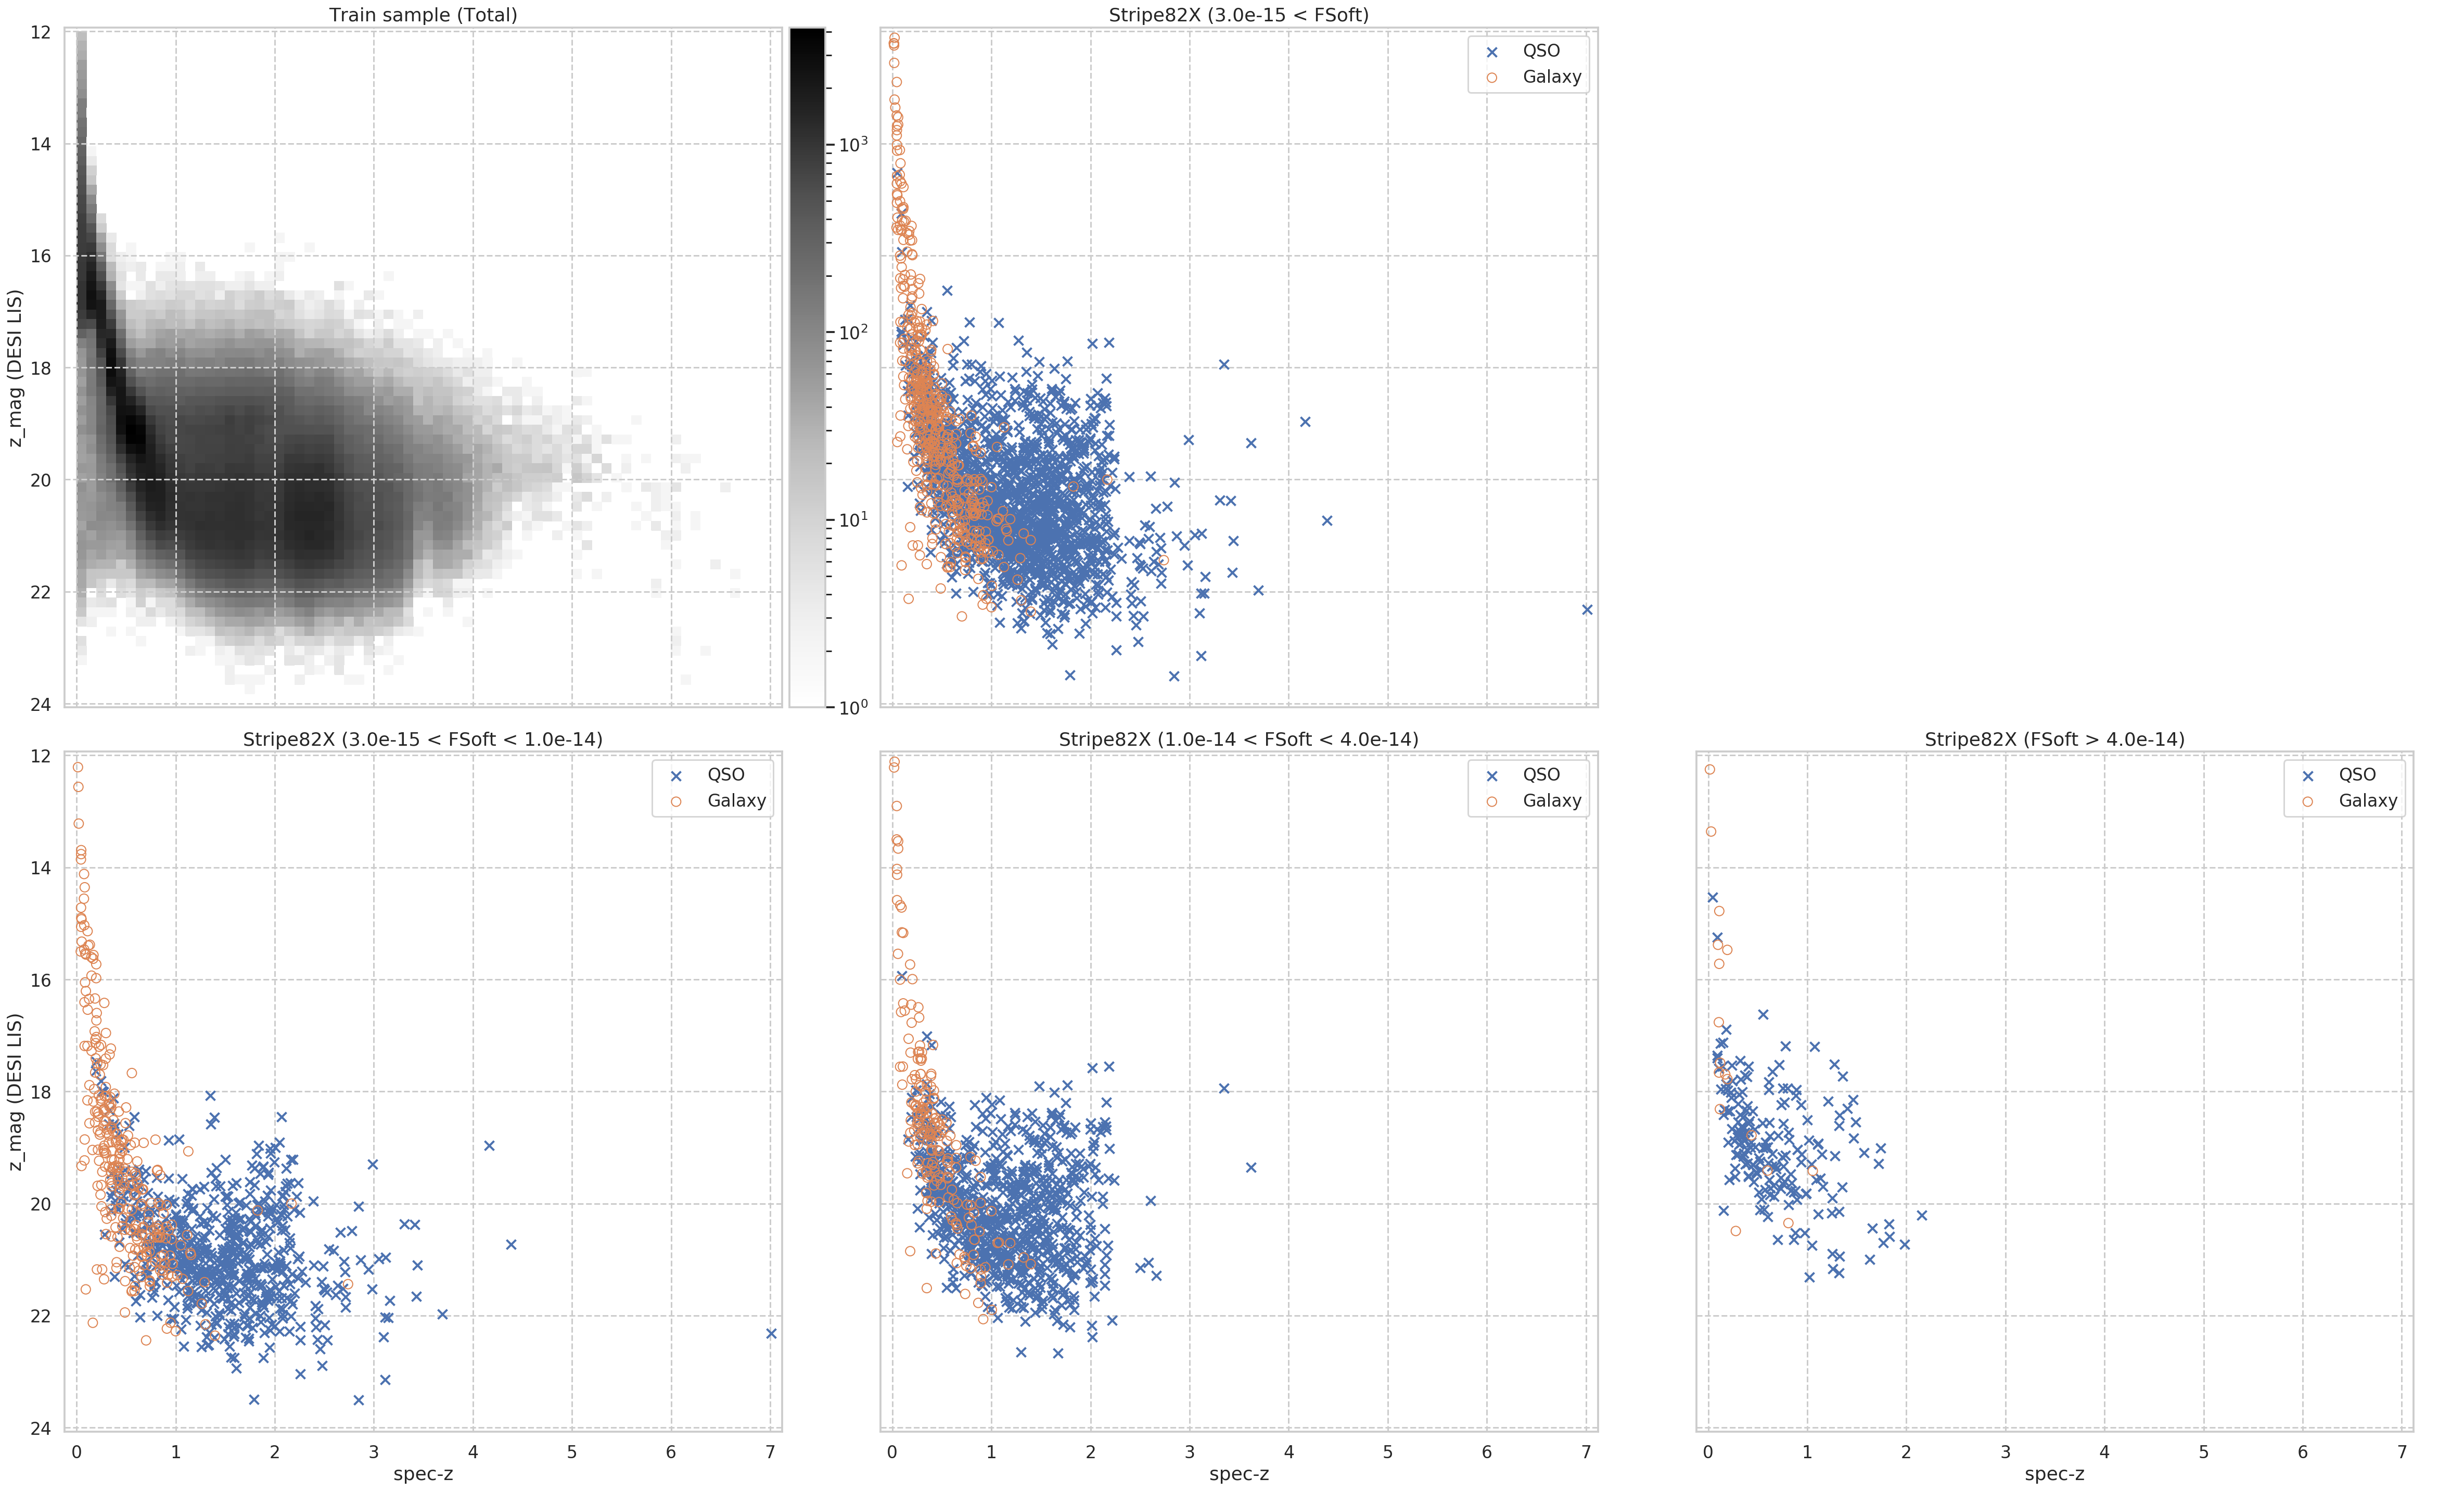
\includegraphics[width=0.95\linewidth]{images/data-dist-ab-upsidedown-s82x.png}
    \caption{The distributions of the objects in the used samples. The abscissa axis is the spectral redshift, the ordinate axis is the value \eqref{eq:mag_ab} in the $z$ filter. The upper line of the graphs, from left to right, is the distributions of galaxies and quasars in the training sample and the test sample of SDSS DR16q quasars.  The bottom line of the graphs is the distribution of Stripe82X objects with different X-ray fluxes. Orange circles show galaxies, blue crosses show quasars.}
    \label{fig:data_distribution}
\end{figure*}

% ===============================================================================
% ============================== The algorithm ==================================
% ===============================================================================

\section{Photo-z model}\label{sec:thealgorithm}

\subsection{Probabilistic regression}
To formulate a probabilistic regression problem, consider a probabilistic formulation of the regression problem. Let \(X\) be the set of object descriptions (feature space), \(Y\) be the target variable definition area. Let represent objects and target variable as random variables \(\xi : \Omega \rightarrow X, \eta : \Omega \rightarrow Y \). Then the process generating the data will be represented as a joint distribution \((\xi, \eta) \sim p(x, y)\). Let the training sample be given \(\mathcal{D}_n = (X_i, y_i)_{i=1}^n \sim p(x,y)\). Under the condition of homoscedasticity and normal distribution of errors on predictors, the regression problem is to construct an estimate of the conditional mean
\begin{equation}\label{eq:regr_classic}
     \hat{y} = \mathbb{E}[\eta | \xi = x] = \int_Y y ~ \hat{p}(y|x) ~ dy
\end{equation}

In the photometric redshift prediction problem, the errors are heteroscedastic. Moreover, the predictors are insufficiently informative (an example is to distinguish a red dwarf and a distant quasar by photometry), which leads multimodal predictive distributions $\hat{p}(y|x)$ and the estimate of the mean will be inadequate. That is why it is necessary to calculate confidence intervals. Therefore, it is necessary to construct a complete distribution $\hat{p}(y|x)$ for each object $x$.

Thus, the task of constructing a probabilistic regression is to train the operator \(\hat{\eta} : X \rightarrow \mathcal{P} \subset L^2\)
\begin{equation}
    \hat{\eta}(x) = \hat{p}(y|x) \in \mathcal{P},
\end{equation}
where \(\mathcal{P}\) is the set of bounded functions satisfying the properties of the probability density function, i.e.
\begin{equation}
    \forall p \in \mathcal{P}, y \in Y, x \in X \Rightarrow p(y|x) \geq 0,
\end{equation}
\begin{equation}
    \forall p \in \mathcal{P}, x \in X \Rightarrow \exists \int_{-\infty}^{+\infty} p(y|x) dy = 1.
\end{equation}

Ideally, as the training sample size \(n\) increases, the solution \(\hat{p}(y|x)\) of the problem should converge to the density function of the original generating process \(p(x|y) = \frac{p(x,y)}{p(x)}\). However, the generating process is not explicitly known: only the training sample and the test sample, on which the quality will be evaluated, are known.

\subsection{Point, interval and fully probabilistic predictions}
To give an specific value we define point prediction as the prime mode of predicted distribution:\begin{equation}\label{eq:point-estimate}
    \hat{y}(x) = \arg\max_y \hat{\eta}(x) = \arg\max p(y|x).
\end{equation}

Interval prediction given confidence level $\alpha$ is defined as highest probability density interval (HPDI). Thus it contains intervals with highest possible probability density, and integral of probability density function over those intervals equals to $\alpha$, i.e:
\begin{equation}\label{eq:hdpi_def}
    \exists p_\alpha \in \mathbb{R}: HDPI_{\alpha} = \{y : \hat{p}(y|x) \geq p_{\alpha}\}
\end{equation}
and
\begin{equation}
    \int_{HDPI_{\alpha}} \hat{p}(y|x) ~ dy = \alpha.
\end{equation}

A measure of confidence zConf is defined as probability contained in small interval around point prediction i.e.:\begin{equation}\label{eq:zconf}
    zConf(x) = \int_{\frac{|y(x) - \hat{y}(x)|}{1 + y(x)} < 0.06} \hat{p}(y|x)dy ~ (y(x) \geq 0).
\end{equation}

The quality criteria for probabilistic predictions -- accuracy and calibration.

Accuracy is defined for point predictions and can be estimated via RMSE or NMAD metrics. In terms of calibration we expect that???

Those two criteria can't be achieved simultaneously. This is demonstrated by two dummy models.

Let us consider that the true value of the target feature is returned as the prediction (in terms of distributions it can be delta-functions with an integral equal to 1. It is 100\% accurate, but the actual confidence level of confidence intervals with any given confidence level (e.g. 68\%) would equal to 1. In terms of high calibration we expect that 68\% of the test sample objects will have true value of redshift in contained in 68\% predicted confidence intervals.

On the other hand, we can consider an example of an estimator which gives the distribution of objects in the target sample as a prediction. In this case equality confidence intervals will achieve given confidence level, however, the accuracy of such a model would be quite mediocre.

In this paper we aim to achieve high accuracy in the first place.



\subsection{Random forests for probabilistic photo-z}

\begin{figure*}
    \centering
    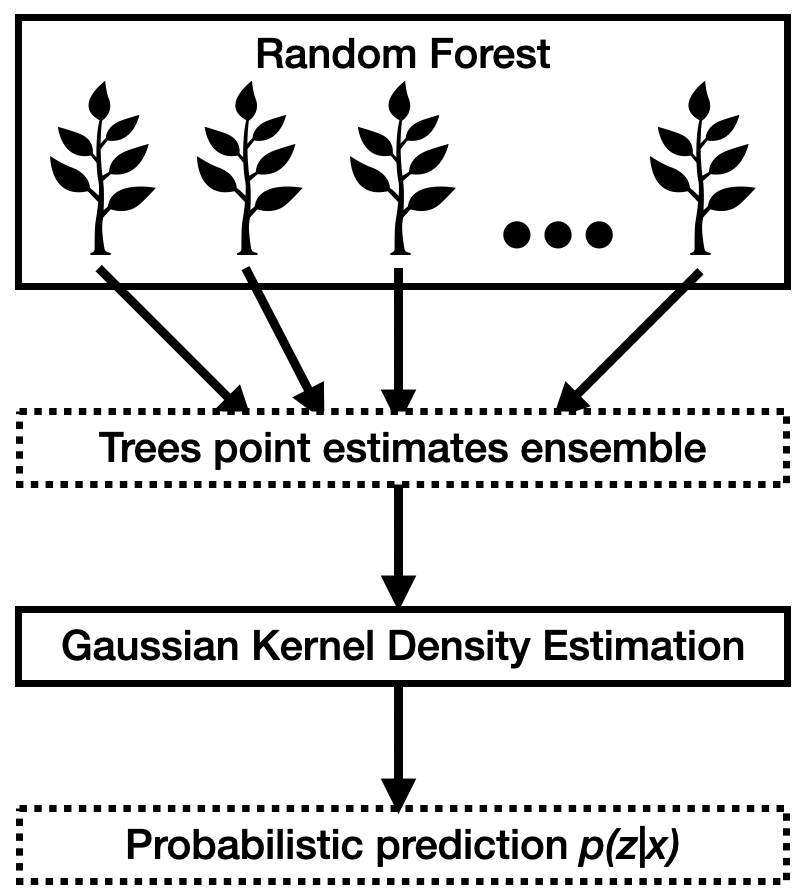
\includegraphics[width=0.55\linewidth]{images/qrf.png}
    \caption{Schematic of the random forest algorithm used, adapted to obtain probabilistic forecasts photo-z.}
    \label{fig:qrf_scheme}
\end{figure*}

\subsubsection{Random forest}
Алгоритм случайного леса для решения задач регрессии классификации был впервые описан в \citep{2001MachL..45....5B} и представляет собой ансамбль деревьев решений $\{A^j\}$, которые строятся независимость. Прогноз случайного леса получается аггрегацией прогнозов всех деревьев. Например, для задачи регрессии итоговый прогноз равен среднему прогнозов деревьев.

Каждое дерево $A^j$ строит разбиение пространства признаков $X$ на непересекающиеся подпространства $A^j_i$, которые в сумме дают все пространство, то есть
\begin{equation}
    \sum_i A^j_i = X, A^j_n \cap A^j_m = \emptyset, m \neq n.
\end{equation}

Построение модели на основе алгоритма случайного леса производится следующим образом. Пусть дана обучающая выборка размера $N$:
\begin{equation}\label{eq:train_sample}
    \mathcal{D} = (\mathcal{D}_X, \mathcal{D}_y),
\end{equation}
\begin{equation}\label{eq:train_features}
    \mathcal{D}_X = (x_{i,j})_{j=1}^M,
\end{equation}
\begin{equation}\label{eq:train_target}
    \mathcal{D}_y = (y_i),
\end{equation}
где $\mathcal{D}_X$ и $\mathcal{D}_y$ признаки и разметка объектов обучающей выборки, соответственно; $i=\overline{1, N}$. Для построения очередного дерева:
\begin{itemize}
    \item бутстрепом генерируется случайная подвыборка $\mathcal{D}^j$ обучающей выборки \eqref{eq:train_sample},
    \item при каждом разбиении в $j$-ом дереве случайно выбираются случайные $m$ признаков из \eqref{eq:train_features}, $m < M$,
    \item для очередного разбиения по заданному критерию определяются оптимальный из $m$ отобранных признаков и пороговое значение,
    \item разбиения строятся пока не исчерпается вся выборка $\mathcal{D}^j$ (дерево без ограничения глубины) или до выполнения определенного условия (в каждом листе осталось не более $n_{min} \in \Theta$ объектов или достигнута заданная высота дерева $h_{max} \in \Theta$.
\end{itemize}

Впервые для задачи вероятностной регрессии был использован в работе \cite{JMLR:v7:meinshausen06a} для точечной оценки квантилей. Построение модели заключается в обучении случайного леса с квантильной функцией потерь 
\begin{equation}\label{eq:quantile_loss}
    l(y_i, \hat{q}_{\alpha, i}) = (1-\alpha)|y_i - \hat{q}_{\alpha, i}|\mathbb{I}[y_i \leq \hat{q}_{\alpha, i}] + \alpha|y_i - \hat{q}_{\alpha, i}|\mathbb{I}[y_i > \hat{q}_{\alpha, i}],
\end{equation}
% \begin{equation}\label{eq:quantile_loss}
%     l(y_i, \hat{q}_{\alpha, i}) = \left\{\begin{array}{rcl}
%          \alpha|y_i - \hat{q}_{\alpha, i}| & y_i > \hat{q}_{\alpha, i} \\
%          (1-\alpha)|y_i - \hat{q}_{\alpha, i}| & y_i \leq \hat{q}_{\alpha, i}
%     \end{array}\right.,
% \end{equation}
где $y_i$ - истинное значение, $\hat{q}_{\alpha, i}$ - предсказанное значение квантиля заданного уровня значимости $\alpha$.

(Дописать критерии разбиения!)

В работе \ref{} проводится анализ поведения случайного леса при различных параметрах рандомизации. Функцию потерь можно разложить на 2 составляющие (так называемый Bias-Variance-Tradeoff:
\begin{equation}\label{eq:bias-variance-tradeoff}
    L = Bias + Variance,
\end{equation}.
Сами по себе деревья решений являются несмещенными $Bias = 0$, но имеют высокий Variance. Путем усреднения ансамбля прогнозов удается понизить Variance.

\subsubsection{Случайный лес как обобщенный метод ближайших соседей}

\subsubsection{Gaussian Kernel Density Estimator}
Gaussian Kernel Density Estimator (KDE) is a non-parametric way model, that estimated probability density function of a random variable. Given a random sample $\{y_i\}_{i=1}^{n_{sample}}$, generated by true distribution of the random variable $y$, the density function estimate is calculated as\begin{equation}\label{eq:kde}
    \hat{p}_i (y) = GKDE(\{y_i\}_{i=1}^{n_{sample}}, h) = \frac{1}{n_{sample} h}\sum_{i=1}^{n_{sample}} K(\frac{y - y_i}{h}),
\end{equation}
\begin{equation}\label{eq:gaussian_kernel}
    K(x) = \frac{1}{\sqrt{2\pi}} * \exp{(-\frac{1}{2} x^2)}.
\end{equation}
where $h$ is the kernel width parameter.

\subsection{SRGz photo-z model}

Random Forests adoptation for probabilistic photo-z via Gaussian KDE.

This method is described in (Meshcheryakov, 2018). The random forest without depth constraint has been adapted for probabilistic predictions by applying kernel density estimation with a Gaussian kernel to the ensemble of tree forecasts. Thus, the prediction for object $x_i$ is a non-parametric estimate of the density of the conditional distribution:
\begin{equation}\label{eq:predproba}
    \hat{p}_i (y) = \hat{p}(y|x_i) = GKDE(\{\hat{y}^{(j)}_i\}_{j=1}^{n_{trees}}, h).
\end{equation}

This approach has the following theoretical interpretation: the independence and randomness of the tree construction allows us to consider the ensemble of tree predictions $\{\hat{y}^{(j)}_i\}_{j=1}^{n_{trees}}$ as a random sample generated by the true distribution $p(y|x_i)$. Thus \eqref{eq:kde} is an estimate of this distribution. A schematic of the method used is shown in Figure \ref{fig:qrf_scheme}.

\subsubsection{Model training and testing procedure}


\subsubsection{Photometric features}
To build Photo-z models, we construct an expert set of features. To do this, we first calculate hyperbolic magnitudes from fluxes:
\begin{equation}\label{eq:asinhmag}
    mag = \Bigg[asinh\Bigg(\frac{f/f_0}{2 \times b/f_0}\Bigg) + \log(b/f_0)\Bigg] \times \Bigg(\frac{-2.5}{\log 10}\Bigg) ~,
\end{equation}
where $f~[nanomaggies]$ и $b = \sigma_{flux}~[nanomaggies]$ - value and error of flux, and (\url{https://www.legacysurvey.org/dr9/description/#photometry})
\begin{equation}
    f_0 = 1~[nanomaggie] = 10^{-(48.6+22.5)/2.5}~[erg/cm^2/Hz].
\end{equation}
Magnitudes values makes it possible to use information about objects with negative fluxes. In addition, the values calculated by this formula contain information about flux errors. It is important to outline, that in SDSS survey $b$ is a mean error for a sky section, while we take the object's flux error $b = \sigma_{flux}~[nanomaggies]$.

Описать свойства гиперболического синуса.

However, we will give all charts in more standard AB-values, which are calculated by the following formula: the formula is taken from here: \url{https://www.sdss.org/dr12/algorithms/magnitudes/} (звезда яркосьтю 1 nanomaggie имеет величину 22.5 \url{https://www.sdss.org/dr12/help/glossary/#mag_pogson})
\begin{equation}\label{eq:mag_ab}
    m_{AB} = [22.5 mag] - 2.5 \log_{10} \frac{f}{f_0}
\end{equation}

Table \ref{tab:featuressets} below provides a description of the feature sets. Different models use photometry from different surveys, so the feature set is determined primarily by the source of the photometric data and spitted into magnitudes and colors. Then, if the model uses DESI LIS model magnitudes, we exclude the attributes associated with these magnitudes from the other surveys. That is why each of SDSS and Pan-STARRS features sets are splitted into two (\ref{feats:sdss-mags-1} and \ref{feats:sdss-mags-2}, \ref{feats:sdss-colors-1} and \ref{feats:sdss-colors-2} for SDSS; \ref{feats:ps-mags-1} and \ref{feats:ps-mags-2}, \ref{feats:ps-colors-1} and \ref{feats:ps-colors-2} for Pan-STARRS). For example, if the model uses the r and g mags from DESI LIS, the model r and g mags from the SDSS survey will not be included in the model, nor will the r-g color based on the SDSS model values. However, because of the absence of PSF magnitudes in DESI LIS, colors like $r_{psf} - r_{cmodel}$ and $r_{psf} - g_{psf}$ based on SDSS magnitudes will be included. Similarly for the Kron magnitudes of the Pan-STARRS surveys.

Models are presented in Table \ref{tab:models}. In total, we present 5 models: model \ref{model:pw} based on Pan-STARRS and WISE photometry, model \ref{model:pdw} based on Pan-STARRS, DESI LIS and WISE photometry, model \ref{model:dw} based on DESI LIS and WISE photometry, model \ref{model:psw} based on SDSS, Pan-STARRS and WISE photometry and model \ref{model:spdw} based on photometry from all four sources.

We use 2 sources of WISE photometry: DESI LIS survey and forced photometry for Pan-STARRS1 survey (Burenin et.al., 202X). The second must be used primarily for model \ref{model:pw}, since using WISE from DESI LIS, which has much less coverage than Pan-STARRS, the goal of building this model -- a forecast over the entire Russian eRosita sky -- will not be achieved.

\begin{table*}
    \label{tab:featuressets}
    \caption{Description of the sets of features used. The first column contains the name of the feature set, the second column contains the feature set number, and the third column lists the magnitudes in the format $passband_{survey, type}$ (for DESI LIS magnitudes -- $passband_{LS}$) and colors based on those magnitudes in the format $mag_1 - mag_2$ that are part of the feature sets. Magnitudes are calculated by the hyperbolic sine formula \eqref{eq:asinhmag}. <<LS>> stands for <<DESI LIS>> and <<PS>> stands for Pan-STARRS1.}
    \newcounter{FeatsSetNumber}[figure] 
    \renewcommand{\theFeatsSetNumber}{\arabic{FeatsSetNumber}}
    \setcounter{FeatsSetNumber}{0}
	\begin{tabular}{ r l p{10cm} }
	\hline
	    Features sets & No. & Features \\
    \hline
        \multirow{2}{*}{SDSS mags} & \refstepcounter{FeatsSetNumber}\theFeatsSetNumber\label{feats:sdss-mags-1} & \(u_{psf}\), \(g_{psf}\), \(r_{psf}\), \(i_{psf}\), \(z_{psf}\), \(u_{cmodel}\), \(i_{cmodel}\), \\
         & \refstepcounter{FeatsSetNumber}\theFeatsSetNumber\label{feats:sdss-mags-2} & \(g_{cmodel}\), \(r_{cmodel}\), \(z_{cmodel}\), \\
        \multirow{2}{*}{SDSS colors} & \refstepcounter{FeatsSetNumber}\theFeatsSetNumber\label{feats:sdss-colors-1} & \(u_{psf}-g_{psf}\), \(u_{psf}-r_{psf}\), \(u_{psf}-i_{psf}\), \(u_{psf}-z_{psf}\), \(u_{psf}-u_{cmodel}\), \(g_{psf}-i_{psf}\), \(g_{psf}-g_{cmodel}\), \(r_{psf}-i_{psf}\), \(i_{psf}-z_{psf}\), \(i_{psf}-i_{cmodel}\), \\
         & \refstepcounter{FeatsSetNumber}\theFeatsSetNumber\label{feats:sdss-colors-2} & \(g_{psf}-r_{psf}\), \(g_{psf}-z_{psf}\), \(r_{psf}-z_{psf}\), \(r_{psf}-r_{cmodel}\), \(z_{psf}-z_{cmodel}\) \\
    \hline
        \multirow{2}{*}{Pan-STARRS mags} & \refstepcounter{FeatsSetNumber}\theFeatsSetNumber\label{feats:ps-mags-1} & \(g_{PS,psf}\), \(r_{PS,psf}\), \(i_{PS,psf}\), \(z_{PS,psf}\), \(y_{PS,psf}\), \(i_{PS,kron}\), \(y_{PS,kron}\) \\
         & \refstepcounter{FeatsSetNumber}\theFeatsSetNumber\label{feats:ps-mags-2} & \(g_{PS,kron}\), \(r_{PS,kron}\), \(z_{PS,kron}\) \\
        \multirow{2}{*}{Pan-STARRS colors} & \refstepcounter{FeatsSetNumber}\theFeatsSetNumber\label{feats:ps-colors-1} & \(g_{PS,psf}-i_{PS,psf}\), \(g_{PS,psf}-y_{PS,psf}\), \(r_{PS,psf}-i_{PS,psf}\), \(r_{PS,psf}-y_{PS,psf}\), \(i_{PS,psf}-z_{PS,psf}\), \(i_{PS,psf}-y_{PS,psf}\), \(z_{PS,psf}-y_{PS,psf}\), \(i_{PS,psf}-i_{PS,kron}\), \(y_{PS,psf}-y_{PS,kron}\) \\
         & \refstepcounter{FeatsSetNumber}\theFeatsSetNumber\label{feats:ps-colors-2} & \(g_{PS,psf}-r_{PS,psf}\) \(g_{PS,psf}-z_{PS,psf}\), \(r_{PS,psf}-z_{PS,psf}\), \(g_{PS,psf}-g_{PS,kron}\), \(r_{PS,psf}-r_{PS,kron}\), \(z_{PS,psf}-z_{PS,kron}\) \\
    \hline
        DESI LIS mags & \refstepcounter{FeatsSetNumber}\theFeatsSetNumber\label{feats:ls-mags-1} & \(g_{LS}\), \(r_{LS}\), \(z_{LS}\) \\
        DESI LIS colors & \refstepcounter{FeatsSetNumber}\theFeatsSetNumber\label{feats:ls-colors-1} & \(g_{LS}-r_{LS}\), \(g_{LS}-z_{LS}\), \(r_{LS}-z_{LS}\) \\
    \hline
        WISE mags & \refstepcounter{FeatsSetNumber}\theFeatsSetNumber\label{feats:wise-mags-1} & \(w1\), \(w2\) \\
        WISE colors & \refstepcounter{FeatsSetNumber}\theFeatsSetNumber\label{feats:wise-colors-1} & \(w1-w2\) \\
    \hline
        SDSS + DESI LIS colors & \refstepcounter{FeatsSetNumber}\theFeatsSetNumber\label{feats:sdss-ls-colors-1} & \(g_{cmodel}-g_{LS}\), \(r_{cmodel}-r_{LS}\), \(z_{cmodel}-z_{LS}\) \\
        SDSS + WISE colors & \refstepcounter{FeatsSetNumber}\theFeatsSetNumber\label{feats:sdss-wise-colors-1} & \(u_{cmodel}-w1\), \(u_{cmodel}-w2\), \(g_{cmodel}-w1\), \(g_{cmodel}-w2\), \(r_{cmodel}-w1\), \(r_{cmodel}-w2\), \(i_{cmodel}-w1\), \(i_{cmodel}-w2\), \(z_{cmodel}-w1\), \(z_{cmodel}-w2\) \\
        Pan-STARRS + DESI LIS colors & \refstepcounter{FeatsSetNumber}\theFeatsSetNumber\label{feats:ps-ls-colors-1} & \(g_{PS,kron}-g_{LS}\), \(r_{PS,kron}-r_{LS}\), \(z_{PS,kron}-z_{LS}\) \\
        Pan-STARRS + WISE colors & \refstepcounter{FeatsSetNumber}\theFeatsSetNumber\label{feats:ps-wise-colors-1} & \(g_{PS,kron}-w1\), \(g_{PS,kron}-w2\), \(r_{PS,kron}-w1\), \(r_{PS,kron}-w2\), \(i_{PS,kron}-w1\), \(i_{PS,kron}-w2\), \(z_{PS,kron}-w1\), \(z_{PS,kron}-w2\), \(y_{PS,kron}-w1\), \(y_{PS,kron}-w2\) \\
        DESI LIS + WISE colors & \refstepcounter{FeatsSetNumber}\theFeatsSetNumber\label{feats:ls-wise-colors-1} & \(g_{LS}-w1\), \(g_{LS}-w2\), \(r_{LS}-w1\), \(r_{LS}-w2\), \(z_{LS}-w1\), \(z_{LS}-w2\) \\
    \hline
    \end{tabular}
\end{table*}

\begin{table*}
    \caption{Models description. The first column indicates the model number, the next four columns indicate the photometry sources used by the model (SDSS, Pan-STARRS, DESI LIS, and WISE, respectively). For SDSS, PS, and LS <<+>> means use of survey photometry, skip -- non-use. For WISE, <<LS>> means use of infrared data from DESI LIS, <<RB>> -- forced photometry for the Pan-STARRS survey from the paper (Burenin et.al., 202X). The last column lists the feature sets from Table \ref{tab:featuressets} used to build the models. <<LS>> stands for <<DESI LIS>> and <<PS>> stands for Pan-STARRS1.}
    \label{tab:models}
    \centering
    \newcounter{ModelNumber}[figure] 
    \renewcommand{\theModelNumber}{\arabic{ModelNumber}}
    \setcounter{ModelNumber}{0}
    \begin{tabular}{r c c c c l}
    \hline
        {}                      & \multicolumn{4}{c}{Data} & {}\\
        No. & SDSS & PS & LS & WISE & Feature sets used \\
    \hline
        \refstepcounter{ModelNumber}\theModelNumber\label{model:pw} & & + & & RB & \ref{feats:ps-mags-1}, \ref{feats:ps-mags-2}, \ref{feats:ps-colors-1}, \ref{feats:ps-colors-2}, \ref{feats:wise-mags-1}, \ref{feats:wise-colors-1}, \ref{feats:ps-wise-colors-1} \\ %Pan-STARRS mags (1 and 2) and colors (1 and 2), WISE mags and colors, Pan-STARRS + WISE colors \\
        \refstepcounter{ModelNumber}\theModelNumber\label{model:pdw} & & + & + & LS & \ref{feats:ps-mags-1}, \ref{feats:ps-colors-1}, \ref{feats:ls-mags-1}, \ref{feats:ls-colors-1}, \ref{feats:wise-mags-1}, \ref{feats:wise-colors-1}, \ref{feats:ps-ls-colors-1}, \ref{feats:ps-wise-colors-1} \\ % Pan-STARRS mags (1) and colors (1), DESI LIS mags and colors, WISE mags and colors, Pan-STARRS + DESI LIS colors, Pan-STARRS + WISE colors \\
        \refstepcounter{ModelNumber}\theModelNumber\label{model:dw} & & & + & LS & \ref{feats:ls-mags-1}, \ref{feats:ls-colors-1}, \ref{feats:wise-mags-1}, \ref{feats:wise-colors-1}, \ref{feats:ls-wise-colors-1} \\ % DESI LIS mags and colors, WISE mags and colors, DESI LIS + WISE colors \\
        \refstepcounter{ModelNumber}\theModelNumber\label{model:spw} & + & + & & RB & \ref{feats:sdss-mags-1}, \ref{feats:sdss-mags-2}, \ref{feats:ps-colors-1}, \ref{feats:ps-colors-2}, \ref{feats:wise-mags-1}, \ref{feats:wise-colors-1}, \ref{feats:sdss-wise-colors-1}, \ref{feats:ps-wise-colors-1} \\
        \refstepcounter{ModelNumber}\theModelNumber\label{model:spdw} & + & + & + & LS & \ref{feats:sdss-mags-1}, \ref{feats:sdss-colors-1}, \ref{feats:ps-mags-1}, \ref{feats:ps-colors-1}, \ref{feats:ls-mags-1}, \ref{feats:ls-colors-1}, \ref{feats:wise-mags-1}, \ref{feats:wise-colors-1}, \ref{feats:sdss-wise-colors-1}, \ref{feats:sdss-ls-colors-1}, \ref{feats:ps-wise-colors-1} \\ % SDSS mags and colors, Pan-STARRS mags (1) and colors (1), DESI LIS mags and colors, WISE mags and colors, SDSS + WISE colors, SDSS + DESI LIS colors, Pan-STARRS + WISE colors \\
    \hline
    \end{tabular}
\end{table*}


\subsubsection{Account for extinction}

To account for Galactic extinction, the $E(B-V)$ estimates from the DESI LIS catalog and the $A/E(B-V)$ coefficients from \citep{2011ApJ...737..103S}. The adjusted values of fluxes and errors on fluxes are calculated using the following formulas:
\begin{equation}
    flux_{ebv, pb} = flux_{pb} 10^{0.4 * dm_{pb}},
\end{equation}
\begin{equation}
    \sigma_{flux_{ebv, pb}} = \sigma_{flux_{pb}} 10^{0.4 * dm_{pb}},
\end{equation}
where $dm_{pb} = E(B-V) * [A/E(B-V)]_{pb}$, $[A/E(B-V)]_{pb}$ is coefficient from \citep{2011ApJ...737..103S} for $pb$ filter, $flux_{ebv, pb}$ и $\sigma_{flux_{ebv, pb}}$ are flux and errors on flux in $pb$ filter.

\subsection{Photo-z metrics}

To evaluate the quality of the photo-z point forecasts obtained from the probabilistic forecast, we use 2 metrics standard for the photo-z forecast problem:
\begin{itemize}
    \item normalized median absolute deviation \begin{equation}\label{eq:nmad}
        NMAD = 1.4826 \times median(|\delta z_{norm,i}|)
    \end{equation}
    \item and catastrophic outliers fraction \begin{equation}\label{eq:n015}
        n_{>0.15} = \frac{\#\{i = \overline{1, N} | \delta z_{norm, i} > 0.15\}}{N};
    \end{equation}
\end{itemize}
where \(N\) is the sample size, and the prediction error \begin{equation}\label{eq:dznorm}
    \delta z_{norm,i} = \frac{\Delta z_i}{1+z_{spec,i}} = \frac{\hat{z}_{ph,i} - z_{spec,i}}{1+z_{spec,i}}.
\end{equation}

To assess the quality of confidence interval calibration, the theoretical and actual confidence level of 68 percent confidence intervals can be compared:
\begin{equation}\label{eq:calpha}
    C_{\alpha} = \frac{\#\{i = \overline{1, N} | z_{ph,i} \in CI_{\alpha, i}\}}{N}.
\end{equation}
A perfect calibration will achieve equality
\begin{equation}\label{eq:perfect-ci}
    C_{\alpha} = \alpha ~ \forall \alpha \in [0, 1]
\end{equation}

In this paper, we evaluate the calibration of the 68 percent confidence intervals:
\begin{equation}\label{eq:c68}
    C_{68} - 0.68 = \frac{\#\{i = \overline{1, N} | z_{ph,i} \in CI_{68, i}\}}{N} - 0.68.
\end{equation}

% ===============================================================================
% ================================ Results ======================================
% ===============================================================================
\clearpage

\section{Results}

\subsection{Анализ качества моделей на рентгеновских данных (Stripe82X)}
\begin{enumerate}
	\item Какая модель лучшая на пересечении
	\item Точность модели на всем небе и самой глубокой
	\item На пересечении превосходство в 2 раза
	\item комбинированный прогноз -- превосходство в 1.5 раза (в т.ч. Визуальное сравнение по скаттерплотам (в каких областях получаем меньше прогнозов))
	\item как превосходит на разных популяциях объектов (яркие-слабые, галактики-квазары)
\end{enumerate}

\subsection{Поведение моделей на кросс-валидации и выборке квазаров DR16q}
\begin{enumerate}
	\item На разных красных смещениях модели имеют разнородную точность (смотрим на графики в зависимости от красного смещения)
	\item по красному смещению на ярких-слабых
	\item по красному смещению на галактиках-квазарах
	\item Ошибки второго рода (смотрим на диаграммы рассеяния разных моделей, 35 модель дает меньше всего таких ошибок).
	\item Общая характеристика прогнозов по скаттерплотам (уверенные прогнозы лежат преимущественно на диагонали, выбросы, преимущественно, имеют низкую уверенность)
	\item Точность моделей ухудшается на слабых источниках (смотрим на графики в зависимости от оптической яркости)
	\item Модели дают высокую точность для галактик и значительное число ошибок для близких квазаров (смотрим на метрики галактик и квазаров) (яркие-слабые квазары-галактики)
	\item Ложные уверенные прогнозы (смотрим на диаграммы рассеяния и спектры) (сравнение поведения моделей на квазарах и на кросс-валидации)
\end{enumerate}

\subsection{Характеристика оценок уверенности zConf}
\begin{enumerate}
	\item 2 актуальные задачи отбора объектов (поиск уникальных объектов, доля выбросов не более 20 процентов, и составление выборок с заданной точностью, 4\% выбросов)
	\item Смотрим на графики со всеми объектами и z\_phot > 3 с требованием 20\% выбросов и видим что это требование достигается на zConf == 0.4 для всех моделей.
	\item Смотрим на графики от фотоз в бинах по zConf 
	\item Смотрим на графики и понимаем, что zConf > 0.4 == шлак
\end{enumerate}

\subsection{Точность и полнота прогнозов}
\begin{enumerate}
	\item выбрали zConf в предыдущем пункте
	\item полнота
	\item точность
	\item на рентгеновской выборке
	\item на оптических выборках
\end{enumerate}

\clearpage\clearpage\clearpage\clearpage
\clearpage
\section{Results OLD}



Нашей целью является анализ качества моделей, построенных на разных наборах признаков (подробнее см. в \ref{}), в зависимости от целевой величины (spec-z) \ref{ssec:accuracy-as-fzspec} и наблюдаемых предикторов (звездной величины в фильтре z \ref{ssec:accuracy-as-fzmag}, рентгеновского потока \ref{ssec:accuracy-as-ffx}). Чтобы добиться лучшего разрешения (это особенно актуально для объектов на $z > 3$) мы используем метод двукратной перекрестной оценки и выборку оптических квазаров SDSS DR16q, описанную в разделе \ref{}.

Кроме того важной задачей является оценка точности прогнозов, которым дана высокая уверенность, и потоноты таких прогнозов, что описано в разделе \ref{ssec:precision-and-completeness}.

В конце в разделе \ref{ssec:sota-comp} проводится сравнение представленных моделей с моделями других исследователей на выборке Stripe82X.

% \subsection{Описание демонстративных материалов}
% Результаты представлены на основе трех типов демонстративных материалов:
% \begin{itemize}
%     \item диагарммы рассеяния прогнозов;
%     \item графики зависимости значений метрик качества прогнозов от наблюдаемых и целевой величин;
%     \item таблицы значений метрик в зависимости от от наблюдаемых и целевой величин.
% \end{itemize}

% На диаграммах рассеяния прогнозов сравниваются истинные и предсказанные значения целевой переменной, а цветом и размером маркера показана оценка уверенности модели. Для качественной модели ожидается, что основная масса прогнозов лежит близко к диагонали, и что такие прогнозы имеют высокую оценку уверенности, а прогнозы, лежащие далеко от диагонали (катастрофические выбросы, подробнее см. ниже), имеют низкую оценку уверенности.

% Графики и таблицы метрик необходимы для подробного исследования поведения моделей на разных объектах (слабые -- яркие в оптике или рентгене, далекие -- близкие). Графики метрик приведены для прогнозов на больших выборках (кросс-валидационные прогнозы, выборка объектов DR16q). Каждая точка на графике соответствует интервалу значений признака по оси Х. Разбиение на интервалы строилось таким образом, чтобы в каждый интервал попало примерно одинаковое количество объектов ($\sim$ ??? для кросс-валидации и $\sim$ ??? для тестовой выборки квазаров), и, таким образом, достигался одинаковый уровень шума. Таблицы необходимы для небольших выборок (Stripe82X), где количество объектов не позвоялет построить достаточное количество интервалов, чтобы получить содержательные графики, при этом, с низким уровнем шума. В итоговой таблице даны метрики по всем трем выборкам, чтобы можно было сравнивать поведение моделей на разных выборках в едином формате.

% Помимо этого мы исследуем поведение моделей в терминах точности и полноты (при отборе кандидатов для спектральных наблюдений). Точность определяется как доля объектов с точным прогнозом ($|\delta z_{norm}| < 0.15$) из тех, которые имеют высокую оценку уверенности прогноза ($zConf > 0.4$):\begin{equation}\label{eq:precision}
%     Precision = \frac{\#\{i = \overline{1, N} | \delta z_{norm, i} < 0.15, zConf_i > 0.4\}}{\#\{i = \overline{1, N} | zConf_i > 0.4\}}.
% \end{equation}
% Исследовать точность модели имеет смысл, в первую очередь, в зависимости от photo-z -- какой доли объектов с высокой уверенность прогноза заданное значение photo-z предсказано верно.

% Полнота определяется как доля объектов, имеющая точный и уверенный прогноз:\begin{equation}\label{eq:completeness}
%     Completeness = \frac{\#\{i = \overline{1, N} | \delta z_{norm, i} < 0.15, zConf_i > 0.4\}}{N}.
% \end{equation}
% Исследовать полноту стоит в зависимости от spec-z -- какую долю объектов на заданном spec-z мы обнаружим по прогнозам моделей.

\clearpage

\subsection{Сравнение точности photo-z рентгеновских источников на выборке Stripe82X}\label{ssec:sota-comp}

\underline{Сравнение с Ananna и Brescia. Точность выше в 1.5 раза (TODO разобраться с объектами без прогнзов).}

\subsection{Визуальное сравнение качества прогнозов. В каких областях стал меньше выбросов}

\underline{Точность в зависимости от рентгеновского потока.}

\begin{figure*}
    \centering
    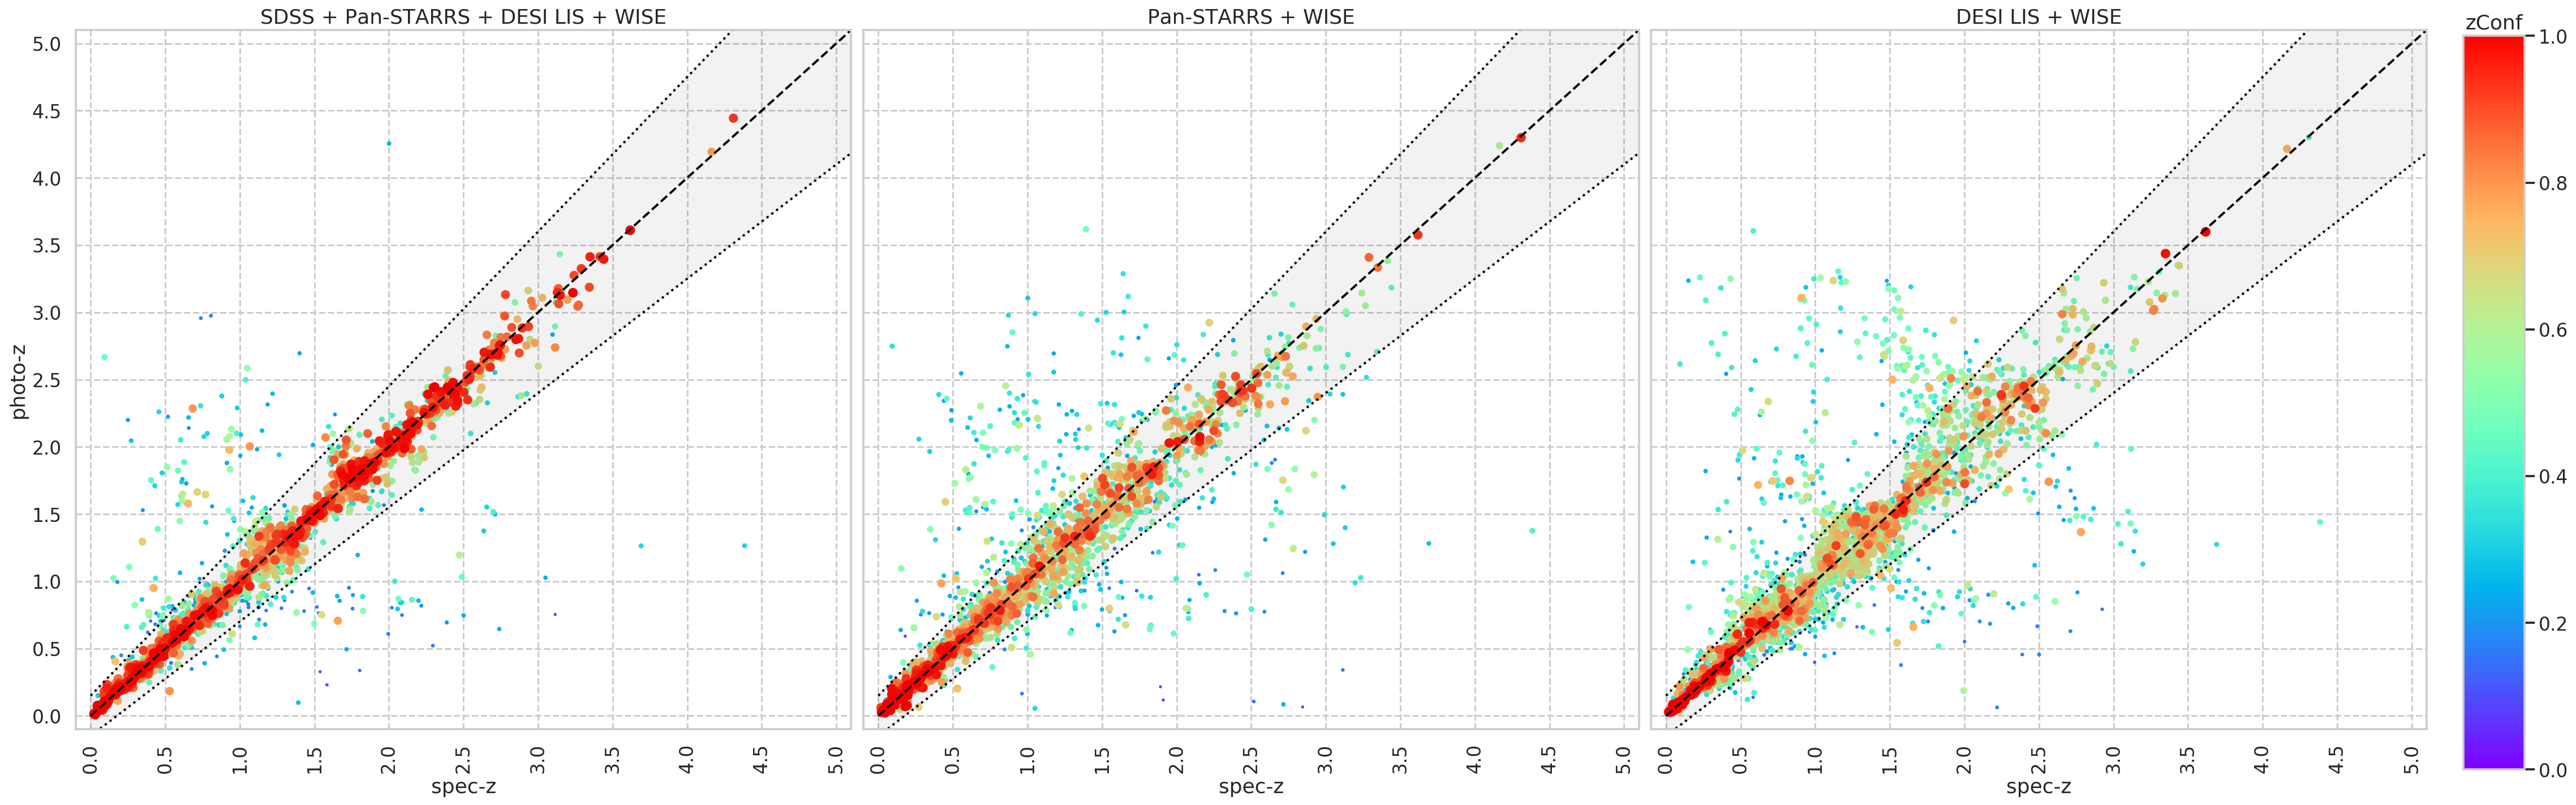
\includegraphics[width=0.99\linewidth]{images/scatterplots-stripe82x-sorted.png}
    \caption{Scatterplots of predictions on Stripe82X X-ray test sample of three models (from left to right) -- \ref{model:spdw}, \ref{model:pw}, \ref{model:dw}. The abscissa axis shows the spectral redshift value, and the ordinate axis shows the photometric redshift prediction. The color and size of dots show the prediction reliability zConf \eqref{eq:zconf}. The gray area around the diagonal is the area of predictions that are not catastrophic emissions according to metric \eqref{eq:n015}.}
    \label{fig:scatter-s82x}
\end{figure*}

\begin{figure*}
    \centering
    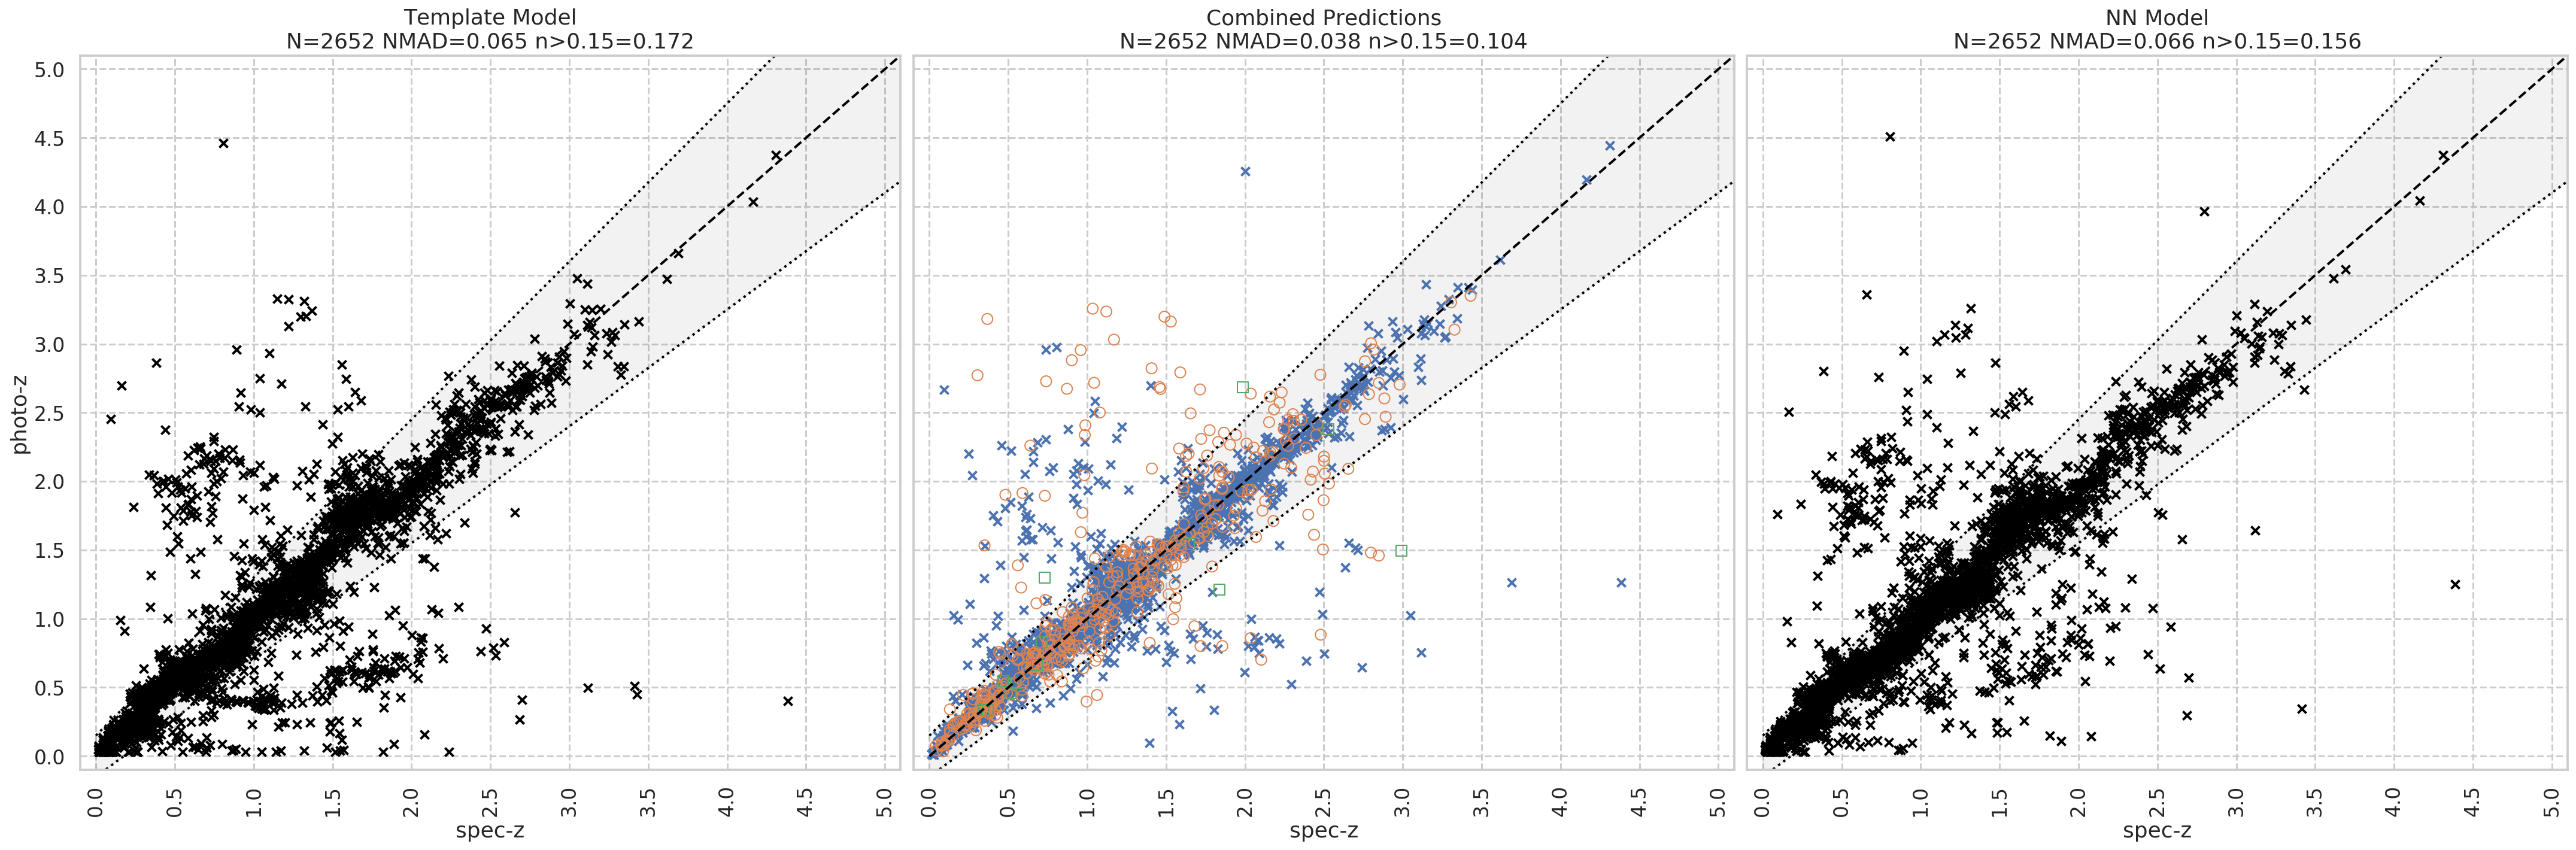
\includegraphics[width=0.9\linewidth]{images/stripe82x-sota35-colored_final.png}
    \caption{Scatterplots of predictions of template model (Ananna, 2017), combined prediction of models \ref{model:pw} -- \ref{model:spdw}, neural network model (Brescia, 2019) on Stripe82X X-ray test sample with $FSoft > 3e-15$ (from left to right). The abscissa axis shows the spectral redshift value, and the ordinate axis shows the photometric redshift prediction. The gray area around the diagonal is the area of predictions that are not catastrophic emissions according to metric \eqref{eq:n015}. The number of predictions with each model in combined predictions is following: \ref{model:spdw} -- 2197, \ref{model:dw} -- 442, has no prediction, comparing to Ananna and Brescia -- 11.}
    \label{fig:scatter-s82x-sota35}
\end{figure*}

\begin{table*}
	\begin{tabular}{llllllllll}
            \hline
            {} & \multicolumn{3}{l}{$FSoft \geq 3e-15$ (2170 objects)} & \multicolumn{3}{l}{$FSoft \geq 1e-14$ (1272 objects)} & \multicolumn{3}{l}{$FSoft \geq 4e-14$ (207 objects)} \\
            {} &                            $NMAD$ &        $n>0.15$ &  $C_{68} - 0.68$ &                            $NMAD$ &        $n>0.15$ &  $C_{68} - 0.68$ &                           $NMAD$ &        $n>0.15$ & $C_{68} - 0.68$ \\
            Model          &                                   &                 &                  &                                   &                 &                  &                                  &                 &                 \\
            \hline
            \ref{model:pw}             &                             0.056 &           0.149 &            0.025 &                              0.05 &           0.119 &            0.033 &                            0.037 &           0.092 &  \textbf{0.025} \\
            \ref{model:pdw}            &                             0.045 &           0.107 &            0.079 &                             0.042 &           0.094 &            0.076 &                             0.03 &           0.068 &           0.074 \\
            \ref{model:dw}             &                             0.073 &           0.171 &  \textbf{-0.012} &                             0.073 &           0.154 &  \textbf{-0.022} &                            0.074 &           0.135 &          -0.057 \\
            \ref{model:spw}            &                             0.039 &           0.105 &            0.094 &                             0.035 &            0.08 &            0.102 &                   \textbf{0.027} &           0.058 &           0.107 \\
            \ref{model:spdw}           &                    \textbf{0.033} &  \textbf{0.087} &            0.109 &                     \textbf{0.03} &  \textbf{0.073} &            0.117 &                   \textbf{0.027} &  \textbf{0.043} &           0.122 \\
            TM &                             0.065 &           0.174 &           -- &                             0.068 &           0.185 &            -- &                            0.073 &           0.222 &          -0.477 \\
            NN             &                             0.065 &            0.16 &           -- &                             0.067 &            0.17 &           -- &                             0.07 &           0.222 &          -- \\
            \hline
            \end{tabular}
            \caption{Prediction metrics for models \ref{model:pw} -- \ref{model:spdw}, template model (Ananna, 2017) and neural network model (Brescia, 2019) on objects from Stripe82X X-ray test sample that have prediction by every model. The first column shows model, the next three columns -- NMAD \eqref{eq:nmad}, catastrophic outliers fraction \eqref{eq:n015}, and 68\% confidence interval calibration \eqref{eq:c68} metrics for objects with $FSoft < 1e-14$, the second three columns -- for objects with $FSoft < 4e-14$, and the last three columns -- for the entire sample. <<TM>> stands for Template model (Ananna, 2017), and <<NN>> for Neural Network model (Brescia, 2019).}
            \label{tab:stripe82x-intersection}
\end{table*}

\begin{table*}
	\begin{tabular}{llllrlllrlllr}
            \hline
            {} & \multicolumn{4}{l}{$FSoft \geq 3e-15$ (2639 objects)} & \multicolumn{4}{l}{$FSoft \geq 1e-14$ (1494 objects)} & \multicolumn{4}{l}{$FSoft \geq 4e-14$ (239 objects)} \\
            {} &                            $NMAD$ &        $n>0.15$ &  $C_{68} - 0.68$ & $N_{preds}$ &                            $NMAD$ &       $n>0.15$ &  $C_{68} - 0.68$ & $N_{preds}$ &                           $NMAD$ &        $n>0.15$ &  $C_{68} - 0.68$ & $N_{preds}$ \\
            Model                               &                                   &                 &                  &             &                                   &                &                  &             &                                  &                 &                  &             \\
            \hline
            \ref{model:pw}                      &                             0.056 &           0.145 &            0.029 &        2179 &                              0.05 &          0.117 &            0.034 &        1278 &                            0.038 &           0.096 &            0.023 &         209 \\
            \ref{model:pdw}                     &                             0.045 &           0.107 &            0.082 &        2220 &                             0.042 &          0.093 &            0.079 &        1287 &                             0.03 &           0.071 &            0.068 &         210 \\
            \ref{model:dw}                      &                             0.074 &           0.173 &  \textbf{-0.005} &        2639 &                             0.072 &          0.154 &  \textbf{-0.013} &        1494 &                            0.074 &           0.142 &           -0.048 &         239 \\
            \ref{model:spw}                     &                             0.039 &           0.101 &            0.098 &        2159 &                             0.035 &          0.077 &            0.105 &        1268 &                   \textbf{0.027} &           0.058 &            0.107 &         207 \\
            \ref{model:spdw}                    &                    \textbf{0.033} &  \textbf{0.084} &            0.113 &        2197 &                     \textbf{0.03} &  \textbf{0.07} &             0.12 &        1276 &                   \textbf{0.027} &  \textbf{0.043} &            0.118 &         208 \\
            \ref{model:dw} w/o \ref{model:spdw} &                             0.078 &           0.179 &            0.021 &         442 &                             0.067 &          0.156 &             0.04 &         218 &                            0.063 &           0.161 &  \textbf{-0.003} &          31 \\
            CP                                  &                             0.038 &             0.1 &            0.098 &        2639 &                             0.033 &          0.082 &            0.108 &        1494 &                            0.028 &           0.059 &            0.102 &         239 \\
            Template Model                      &                             0.065 &           0.172 &           -- &        2639 &                             0.067 &          0.181 &           -- &        1494 &                            0.074 &           0.218 &           -- &         239 \\
            NN Model                            &                             0.066 &           0.156 &           -- &        2639 &                             0.066 &          0.167 &           -- &        1494 &                            0.071 &           0.222 &           -- &         239 \\
            \hline
            \end{tabular}
            \caption{Prediction metrics for models \ref{model:pw} -- \ref{model:spdw}, template model (Ananna, 2017) and neural network model (Brescia, 2019) from Stripe82X X-ray test sample. The first column shows model, the next three columns -- NMAD \eqref{eq:nmad}, catastrophic outliers fraction \eqref{eq:n015}, and 68\% confidence interval calibration \eqref{eq:c68} metrics for objects with $FSoft < 1e-14$, the second three columns -- for objects with $FSoft < 4e-14$, and the last three columns -- for the entire sample. <<TM>> stands for Template model (Ananna, 2017), <<NN>> for Neural Network model (Brescia, 2019), <<CP>> stands for combined predictions of models \ref{model:spdw} and \ref{model:dw}.}
\end{table*}

\begin{table*}
	\begin{tabular}{lllllrlllrllll}
            \hline
                &    & \multicolumn{4}{l}{$FSoft \geq 3e-15$} & \multicolumn{4}{l}{$FSoft \geq 1e-14$} & \multicolumn{4}{l}{$FSoft \geq 4e-14$} \\
                &    &             $NMAD$ &        $n>0.15$ &  $C_{68} - 0.68$ & $N_{preds}$ &             $NMAD$ &        $n>0.15$ &  $C_{68} - 0.68$ & $N_{preds}$ &             $NMAD$ &        $n>0.15$ &  $C_{68} - 0.68$ & $N_{preds}$ \\
            Obj. Type & Model &                    &                 &                  &             &                    &                 &                  &             &                    &                 &                  &             \\
            \hline
            Galaxy & \ref{model:pw} &              0.047 &           0.116 &  \textbf{-0.017} &         415 &              0.047 &           0.091 &           -0.017 &         175 &                 -- &              -- &               -- &          -- \\
                & \ref{model:pdw} &              0.038 &           0.102 &            0.052 &         422 &              0.037 &            0.08 &   \textbf{0.013} &         176 &                 -- &              -- &               -- &          -- \\
                & \ref{model:dw} &              0.047 &           0.131 &            0.086 &         504 &              0.049 &            0.11 &            0.081 &         209 &                 -- &              -- &               -- &          -- \\
                & \ref{model:spw} &              0.041 &           0.097 &            0.075 &         412 &              0.036 &            0.08 &            0.056 &         174 &                 -- &              -- &               -- &          -- \\
                & \ref{model:spdw} &     \textbf{0.037} &           0.098 &            0.093 &         419 &     \textbf{0.034} &  \textbf{0.074} &             0.08 &         175 &                 -- &              -- &               -- &          -- \\
                & \ref{model:dw} w/o \ref{model:spdw} &               0.05 &           0.129 &            0.155 &          85 &              0.042 &           0.118 &            0.232 &          34 &                 -- &              -- &               -- &          -- \\
                & CP &              0.038 &           0.103 &            0.104 &         504 &     \textbf{0.034} &           0.081 &            0.105 &         209 &                 -- &              -- &               -- &          -- \\
                & TM &              0.069 &           0.095 &           -0.394 &         504 &              0.071 &           0.105 &           -0.441 &         209 &                 -- &              -- &               -- &          -- \\
                & NN &              0.068 &  \textbf{0.085} &           -0.295 &         504 &              0.071 &           0.105 &           -0.369 &         209 &                 -- &              -- &               -- &          -- \\
            QSO & \ref{model:pw} &              0.061 &           0.156 &            0.036 &        1400 &               0.05 &           0.121 &            0.041 &         895 &              0.033 &           0.075 &             0.05 &       159.0 \\
                & \ref{model:pdw} &              0.049 &           0.113 &            0.084 &        1425 &              0.042 &           0.092 &            0.092 &         900 &              0.028 &           0.063 &            0.087 &       159.0 \\
                & \ref{model:dw} &              0.083 &           0.191 &            -0.03 &        1692 &              0.076 &            0.16 &           -0.033 &        1040 &              0.076 &           0.153 &           -0.057 &       183.0 \\
                & \ref{model:spw} &               0.04 &            0.11 &             0.11 &        1386 &              0.035 &           0.081 &            0.112 &         889 &     \textbf{0.025} &            0.05 &            0.138 &       159.0 \\
                & \ref{model:spdw} &     \textbf{0.034} &  \textbf{0.089} &            0.123 &        1409 &      \textbf{0.03} &  \textbf{0.074} &             0.13 &         894 &     \textbf{0.025} &  \textbf{0.038} &             0.15 &       159.0 \\
                & \ref{model:dw} w/o \ref{model:spdw} &              0.085 &           0.191 &  \textbf{-0.023} &         283 &              0.072 &           0.151 &  \textbf{-0.016} &         146 &               0.07 &           0.208 &  \textbf{-0.013} &        24.0 \\
                & CP &               0.04 &           0.106 &            0.099 &        1692 &              0.034 &           0.085 &            0.109 &        1040 &              0.027 &            0.06 &            0.129 &       183.0 \\
                & TM &               0.07 &           0.203 &           -0.303 &        1692 &               0.07 &           0.196 &           -0.356 &        1040 &              0.077 &           0.224 &           -0.472 &       183.0 \\
                & NN &               0.07 &           0.181 &           -0.226 &        1692 &              0.067 &           0.179 &           -0.271 &        1040 &              0.076 &            0.23 &           -0.369 &       183.0 \\
            \hline
            \end{tabular}
            \caption{Точность Stripe82X на разных классах объектов}
\end{table*}

Очередная цель этой статьи -- сравнение с моделями Photo-z, известными в литературе -- шаблонной моделью (Ananna, 2017) и нейросетевой моделью (Brescia, 2019). Для этого модели были протестированы на выборке Stripe82X, и были подсчитаны метрики точности \eqref{eq:nmad} и \eqref{eq:n015} на пересечении множества объектов, для которых удалось получить прогноз всеми моделями. Для наиболее точной модели получены значения метрик $~2$ раза лучше, чем для шаблонной и нейросетевой моделей для объектов $FSoft \geq 3e-15$ (см. табл. \ref{tab:stripe82x-intersection}).

На рисунке \ref{fig:scatter-s82x-sota35} приведены диаграммы рассеяния шаблонной и нейросетевой моделей и комбинированные прогнозы представленных моделей (то есть, если не удалось сделать прогноз лучшей по точности моделей, пытаемся сделать прогноз следующей по точности моделью и т.д.). Видно, что наши модели показывают меньшее число ошибок второго рода (катастрофические выбросы в районе $spec-z ~ 0.5, photo-z ~ 2.0$ и сильно меньшее число выбросов ниже диагонали.

Итоговые значения метрик точности $NMAD, n_{>0.15} = 0.039, 0.104/ 0.067, 0.175/ 0.067, 0.157$ для комбинированного прогноза представленными моделями / шаблонной модели (Ananna, 2017) / нейросетевой модели (Brescia, 2019), соответственно, на 2639 из ??? объектов выборки Stirpe82X с рентгеновским потоком FSoft > 3e-15 для которых имеются прогнозы шаблонной и нейросетевой модели. 

В таблице \ref{tab:stripe82x-intersection} представлены метрики точности представленных пяти моделей на выборке Stripe82X для разных порогов по рентгеновскому потоку $FSoft$. Можно видеть, что точность всех моделей снижается до двух раз при увеличении глубины обзора. Модель \ref{model:dw} показывает однинаковую точность по метрике $NMAD = 0.73 \pm 0.01$, а доля выбросов ухудшается с $0.135$ на объектах $FSoft \geq 4e-14$ до $0.171$ при добавлении объектов $3e-15 \leq FSoft < 4e-14$.

\clearpage

\subsection{Детальный анализ точности моделей photo-z SRGz}

\subsubsection{Поведение моделей на объектах разных классов}

\underline{Зависимость метрик от спектрального красного смещения. Разнородное поведение моделей на разных красных смещениях.}

Визуальный анализ числа выбросов. Явное превосходство 35ой модели, ошибки второго рода.

Причины ошибок первого рода (показать примеры спектров).

%На рис. \ref{fig:metrics-cv2-total} и \ref{fig:metrics-dr16q} слева приведены графики зависимости метрик качества точенчных прогнозов $NMAD$ \eqref{eq:nmad} и $n_{>0.15}$ \eqref{eq:n015} от значения спектрального красного смещения для представленных пяти моделей на кросс-валидации и тестовой выборке квазаров DR16q, соответственно. Основное, что можно заметить на графиках -- разнородность поведения моделей на разных красных смещениях. При этом поведение моделей может как согласовываться (все представленные модели показывают ухудшение точности в области $spec-z \sim 1.2$ по метрике NMAD) так и отличаться в зависимости от используемых данных (добавление в модель данных Pan-STARRS сильно улучшает точность моделей для близких квазаров на $spec-z < 1$ и квазаров на $spec-z \sim 2.3$ по метрике NMAD и уменьшает долю выбросов на $spec-z \sim 1.7$. В области $2.6 < spec-z < 3.7$ наивысшую точность показывают модели с использованием данных SDSS.
%
%На рисунках \ref{fig:scatter-cv2-total} и \ref{fig:scatter-dr16q_wo_train} диаграммы рассеяния прогнозов моделей \ref{model:spdw} и \ref{model:pw} (верхние 2 графика) и \ref{model:pdw} и \ref{model:dw} (нижние 2 графика) на кросс-валидации и для тестовой выборки квазаров DR16q, соответственно. Для моделей \ref{model:pdw} и \ref{model:dw} показаны только объекты, для которых не удалось сделать прогнозы моделью \ref{model:spdw}. На диаграммах видно облако точек, которые отстоят далеко от главной диагонали и выходят за границы серой области -- катастрофические выбросы, согласно метрике \eqref{eq:n015}, то есть ошибка прогноза $dz_{norm}$ \eqref{eq:dznorm} превышает 0.15. Модель \ref{model:pw} имеет крупное облако точек в районе $[0, 3.5] \times [0, 3.5]$. У наиблее точной модели облако точек уменьшается, что особенно заметно на DR16q.
%
%Так же на на диаграммах рассеяния кросс-валидационных прогнозов можно видеть, что наиблее далекие объекты ($6.5 < spec-z < 7.0$) обнаруживаются в большинстве своем только моделью DESI LIS. Прогноз наиболее точной моделью \ref{model:spdw} для таких объектов нельзя сделать ввиду отсутствия или неполноты фотометрии SDSS и/или Pan-STARRS1 для этих объектов.
%
%На диаграммах рассеяния кросс-валидационных прогнозов можно увидеть объекты с ложным уверенным прогнозом $spec-z \sim 0.5$, что особенно заметно в областях $spec-z > 3.5$, где находится небольшое количество объектов. Такие прогнозы связаны с неправильной размекой в данных DR14q.
%
%С точки зрения ошибок второго рода -- когда в контексте отбора далеких квазаров принимается неверная нулевая гипотеза, что объяет имеет красное смещение > 3 -- модель \ref{model:dw} показывает большее количество ошибок (то есть прогноз > 3 и имеет высокую уверенность, при этом лежит высоко над диагональю) по сравнению с \ref{model:pw} и \ref{model:spdw}, что хорошо видно на ддиаграмме рассеяния для DR16q. Но эта же модель показывает лучшую полноту на наиболее далеких объектах (zspec > 6) -- правильные прогнозы модели являются более уверенными по сравнению с моделями \ref{model:pw} и \ref{model:spdw}, которые почти не показывают уверенных прогнозов на таких объектах.

\begin{figure*}
    \centering
    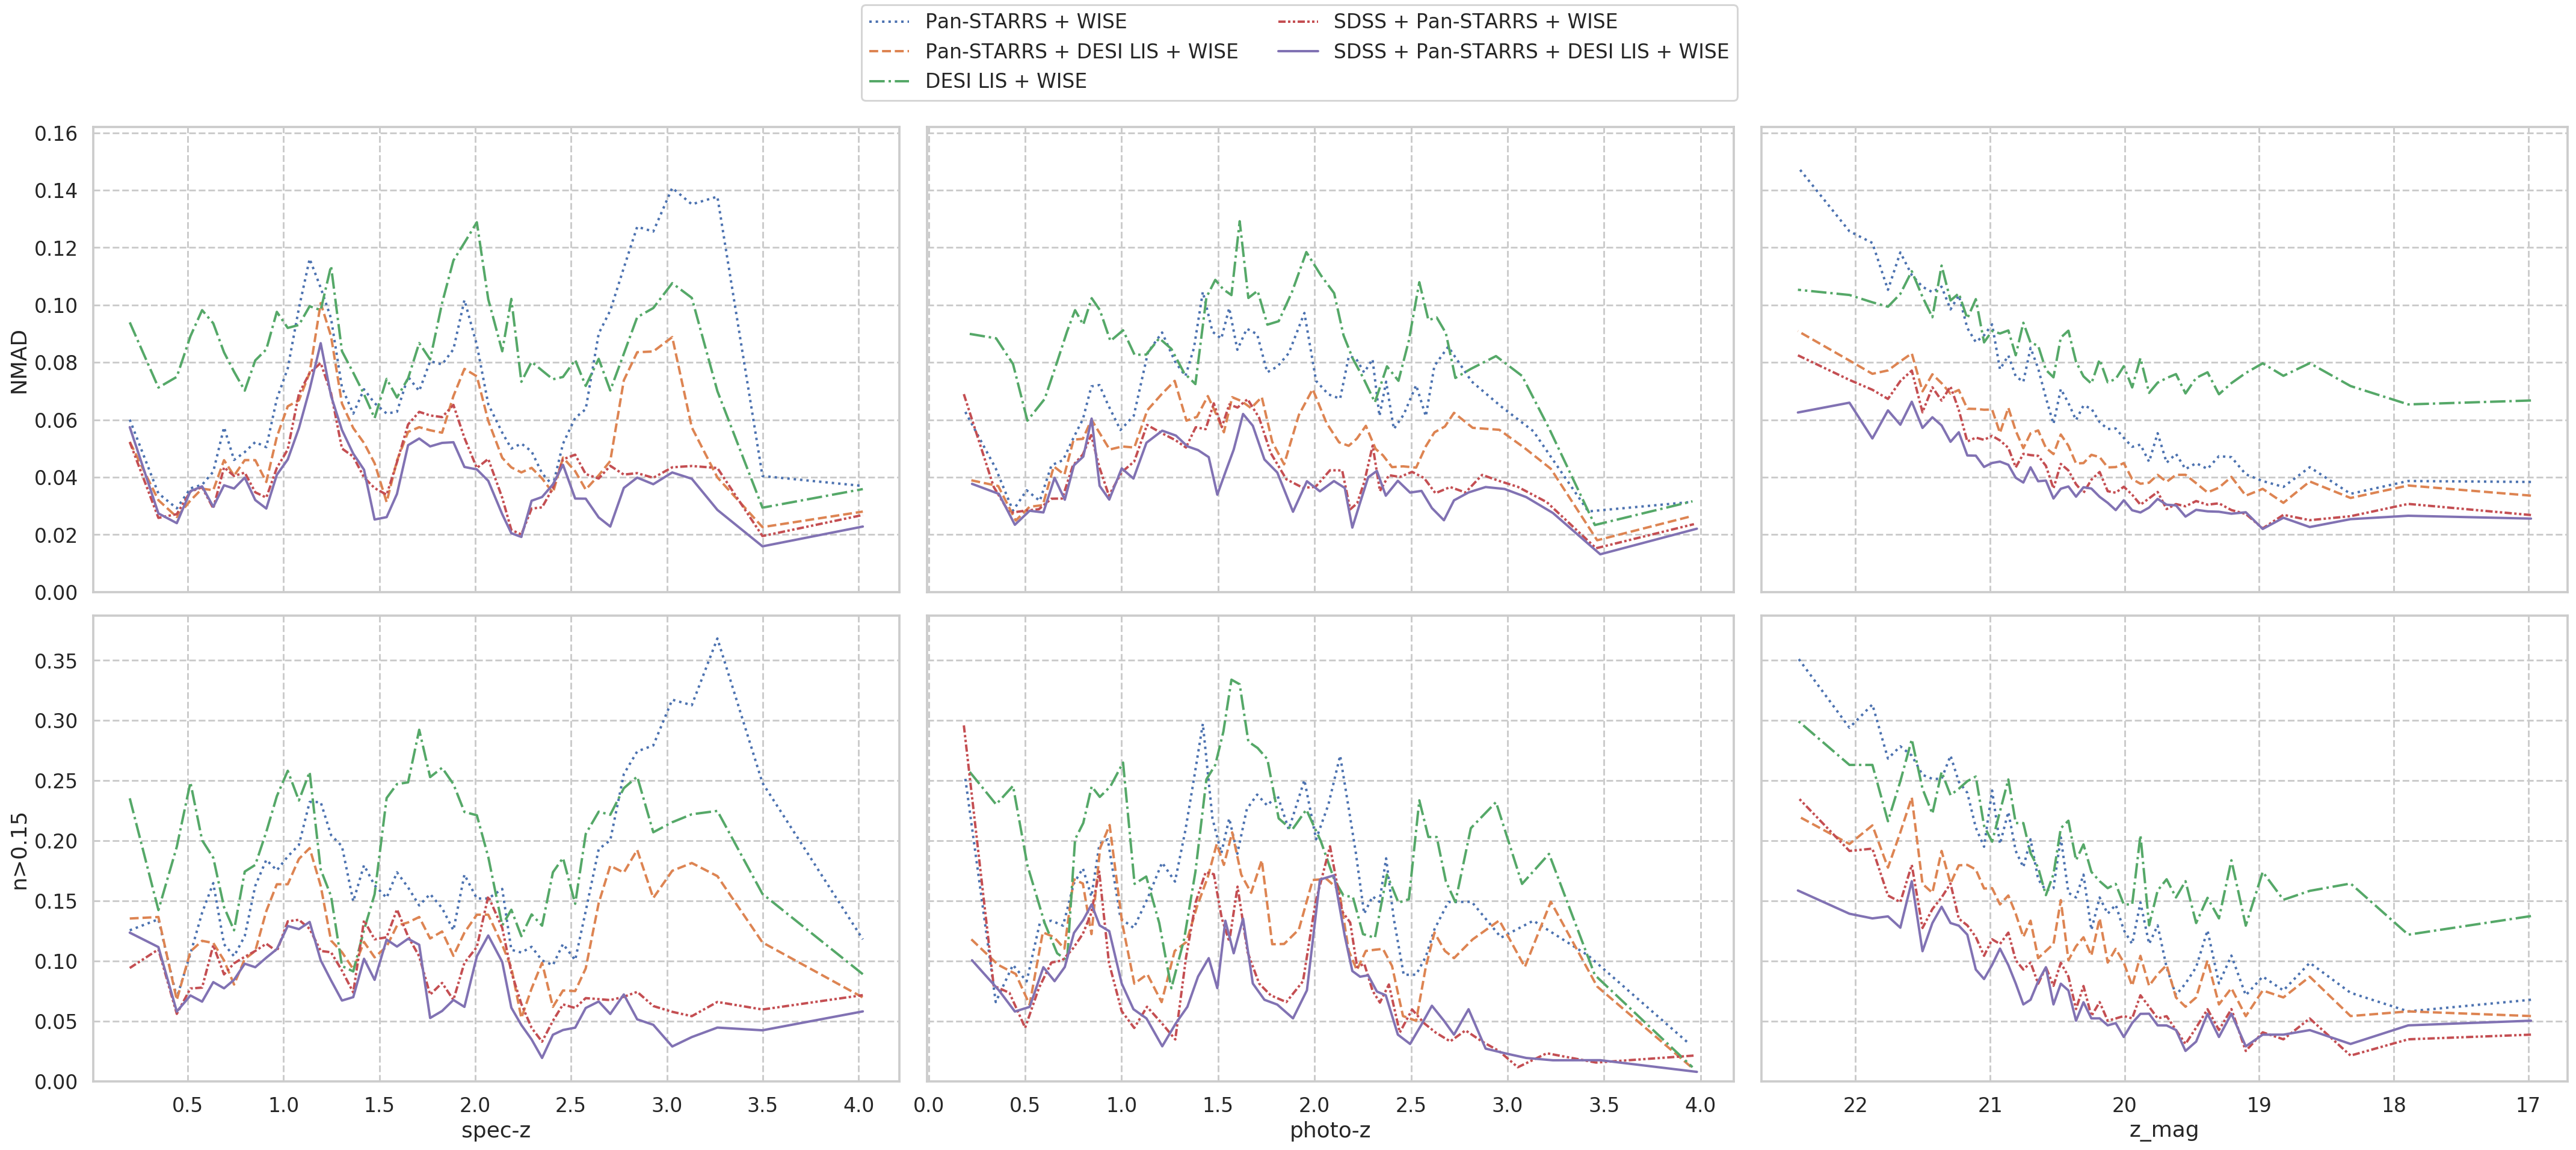
\includegraphics[width=0.99\linewidth]{images/metrics-dr16q-ab-mini.png}
    \caption{Plots of NMAD \eqref{eq:nmad} (upper line of plots) and the fraction of catastrophic outliers \eqref{eq:n015} (lower line of plots) metrics as a function of (from left to right) spectral redshift value, photometric redshift prediction value, and stellar magnitude in the filter z) on DR16q quasars test sample. The solid line shows model \ref{model:spdw}, the dot line shows model \ref{model:pw}, the dashed line shows model \ref{model:pdw}, the dash-dot line shows model \ref{model:dw}, and dash-dot-dot line shows model \ref{model:spw}.}
    \label{fig:metrics-dr16q}
\end{figure*}

\begin{figure*}
    \centering
    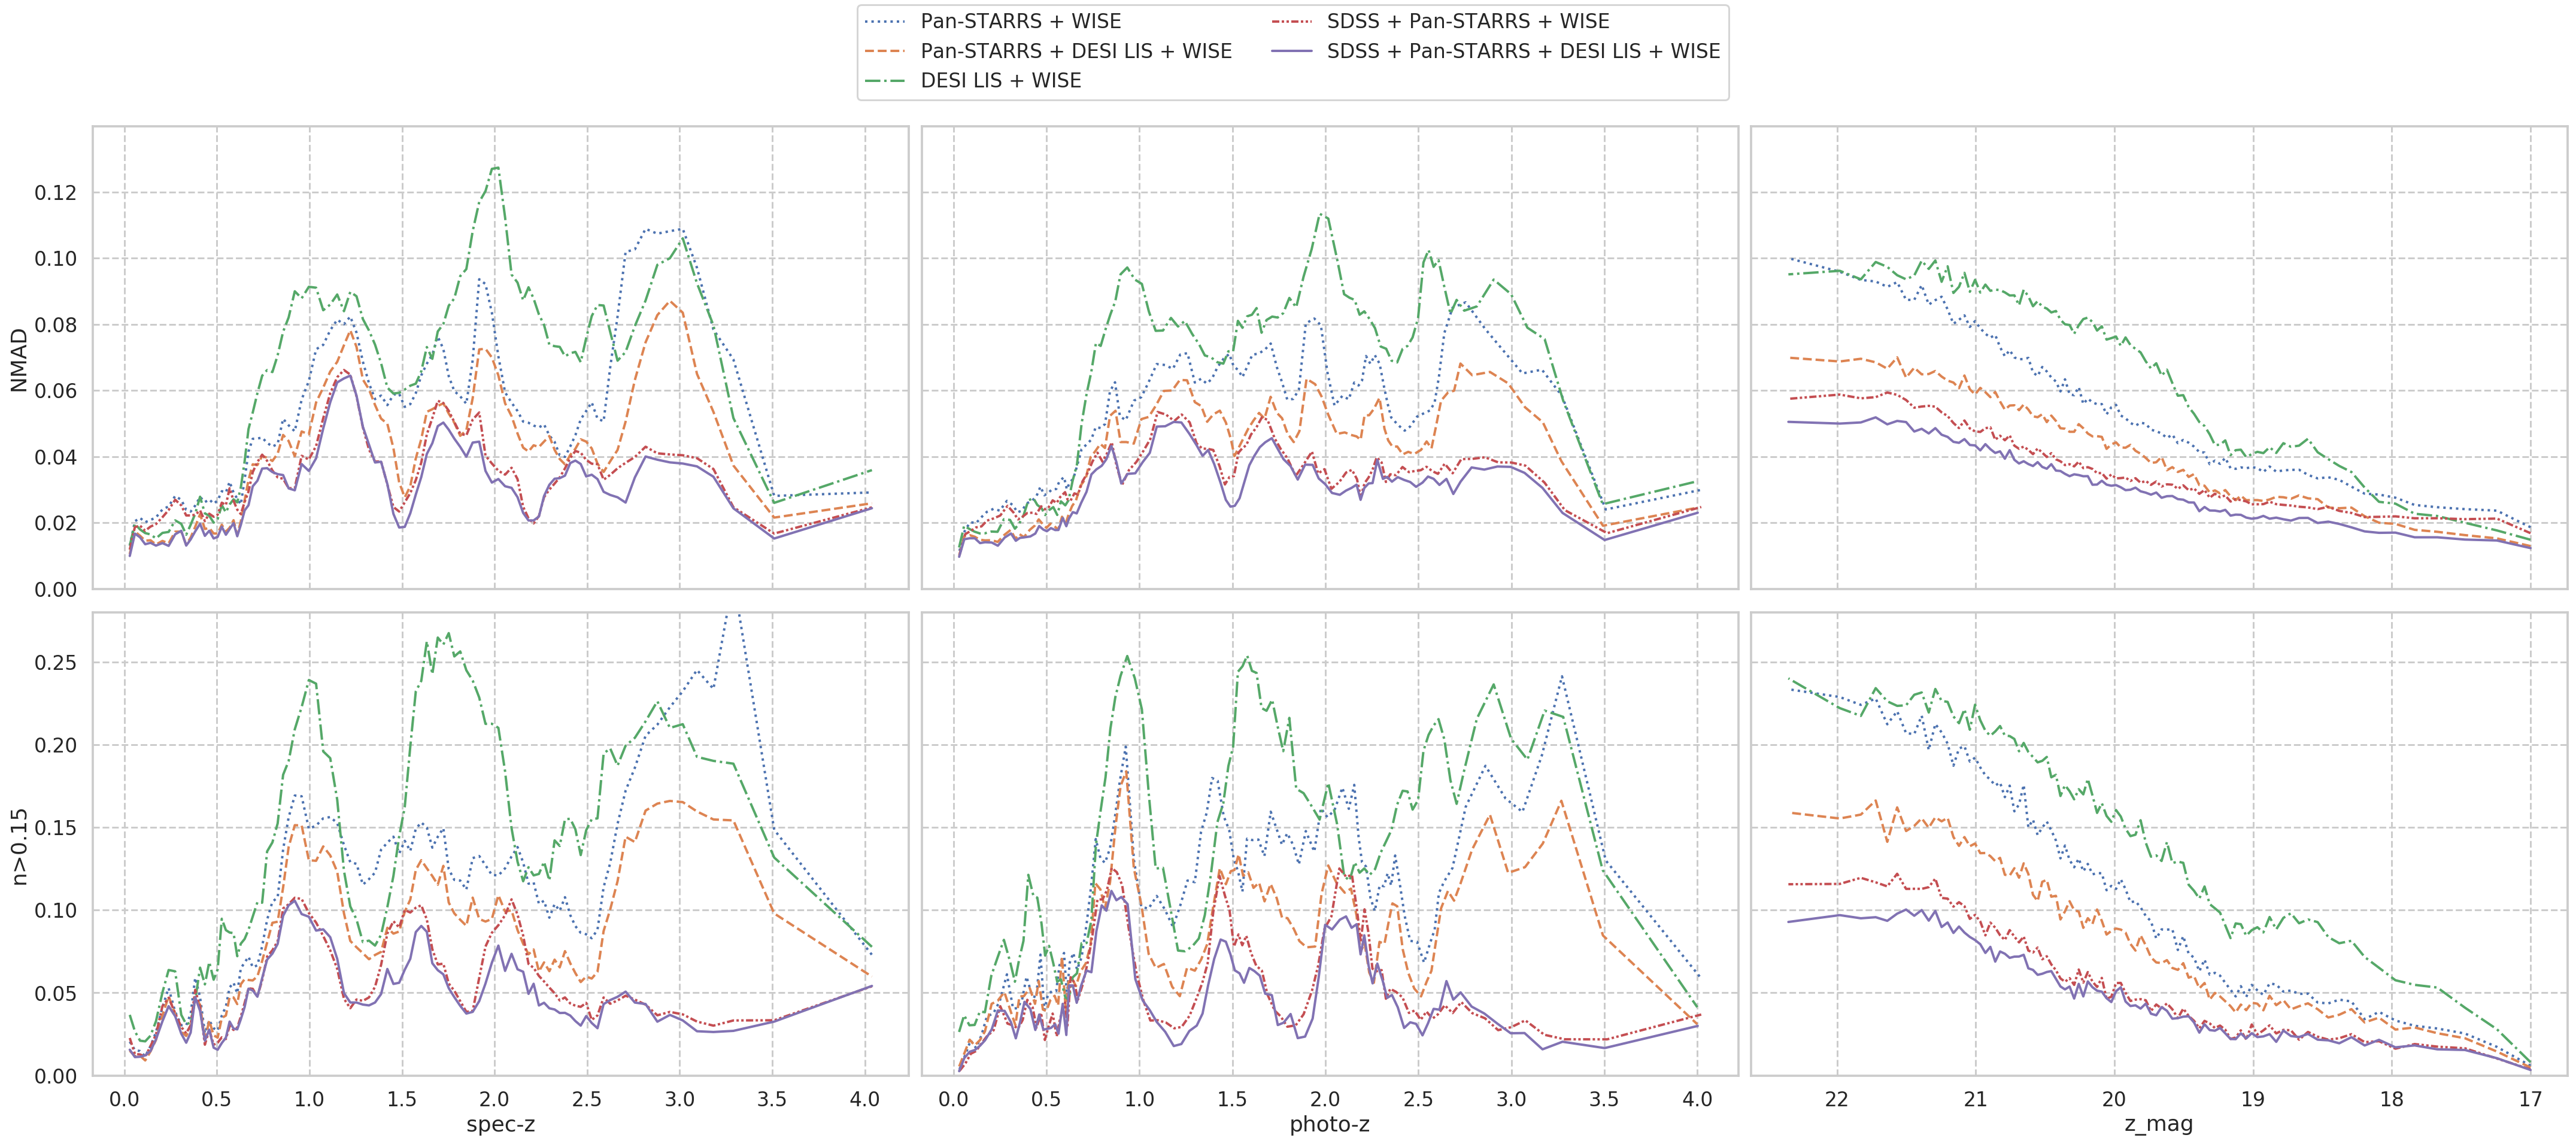
\includegraphics[width=0.99\linewidth]{images/metrics-cv2-ab-mini.png}
    \caption{Plots of NMAD \eqref{eq:nmad} (upper line of plots) and the fraction of catastrophic outliers \eqref{eq:n015} (lower line of plots) metrics as a function of (from left to right) spectral redshift value, photometric redshift prediction value, and stellar magnitude in the filter z) of cross-validation predictions. The solid line shows model \ref{model:spdw}, the dot line shows model \ref{model:pw}, the dashed line shows model \ref{model:pdw}, the dash-dot line shows model \ref{model:dw}, and dash-dot-dot line shows model \ref{model:spw}.}
    \label{fig:metrics-cv2-total}
\end{figure*}

\begin{figure*}
    \centering
    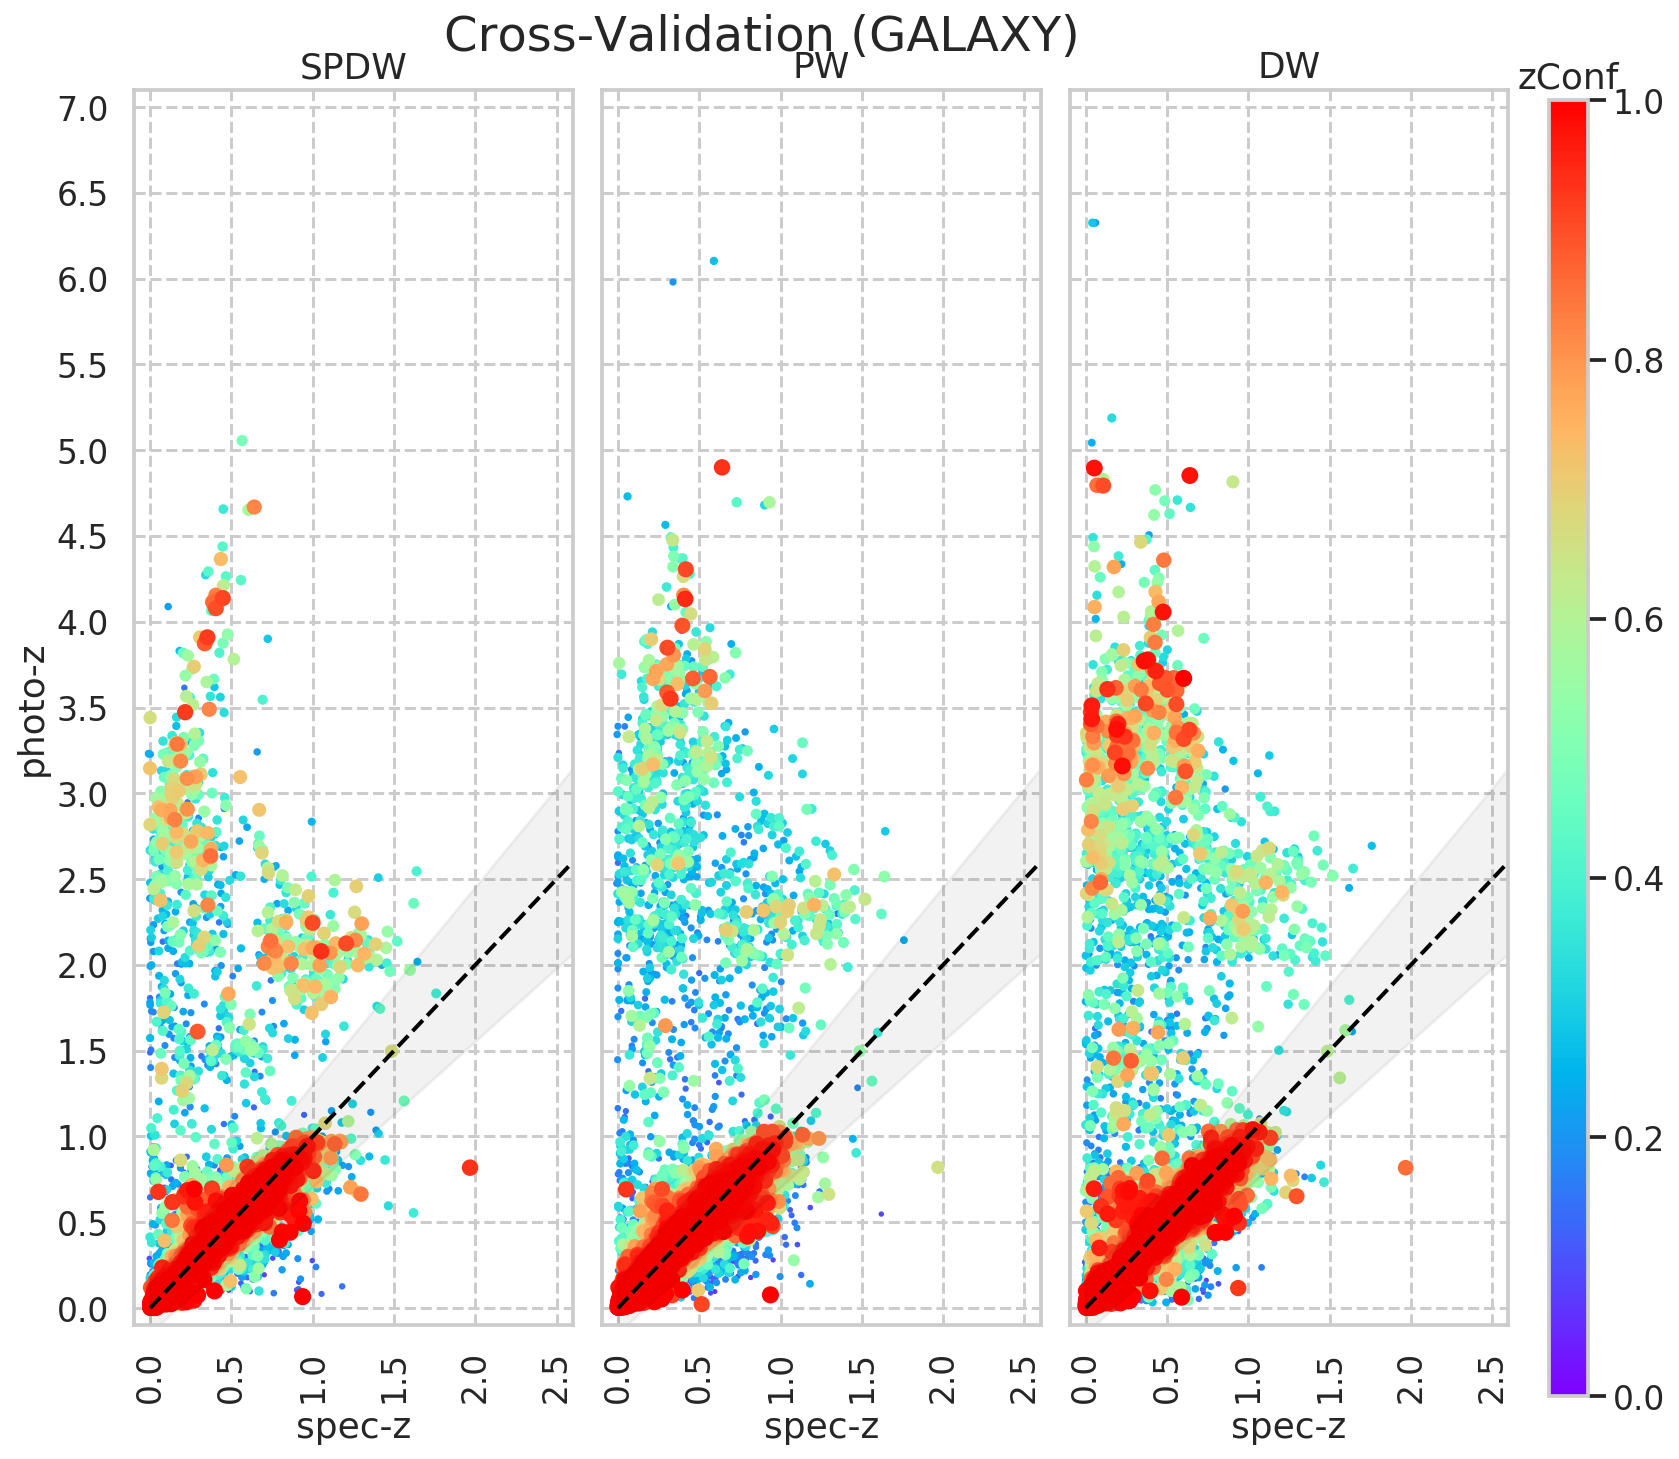
\includegraphics[width=0.55\linewidth]{images/scatterplots-cv2-gal-sorted.png}
    \caption{Scatterplots of cross-validation predictions of galaxies of three models (from left to right) -- \ref{model:spdw}, \ref{model:pw}, \ref{model:dw}. The abscissa axis shows the spectral redshift value, and the ordinate axis shows the photometric redshift prediction. The color and size of dots show the prediction reliability zConf \eqref{eq:zconf}. The gray area around the diagonal is the area of predictions that are not catastrophic emissions according to metric \eqref{eq:n015}.}
    \label{fig:scatter-cv2-gal}
\end{figure*}

\begin{figure*}
    \centering
    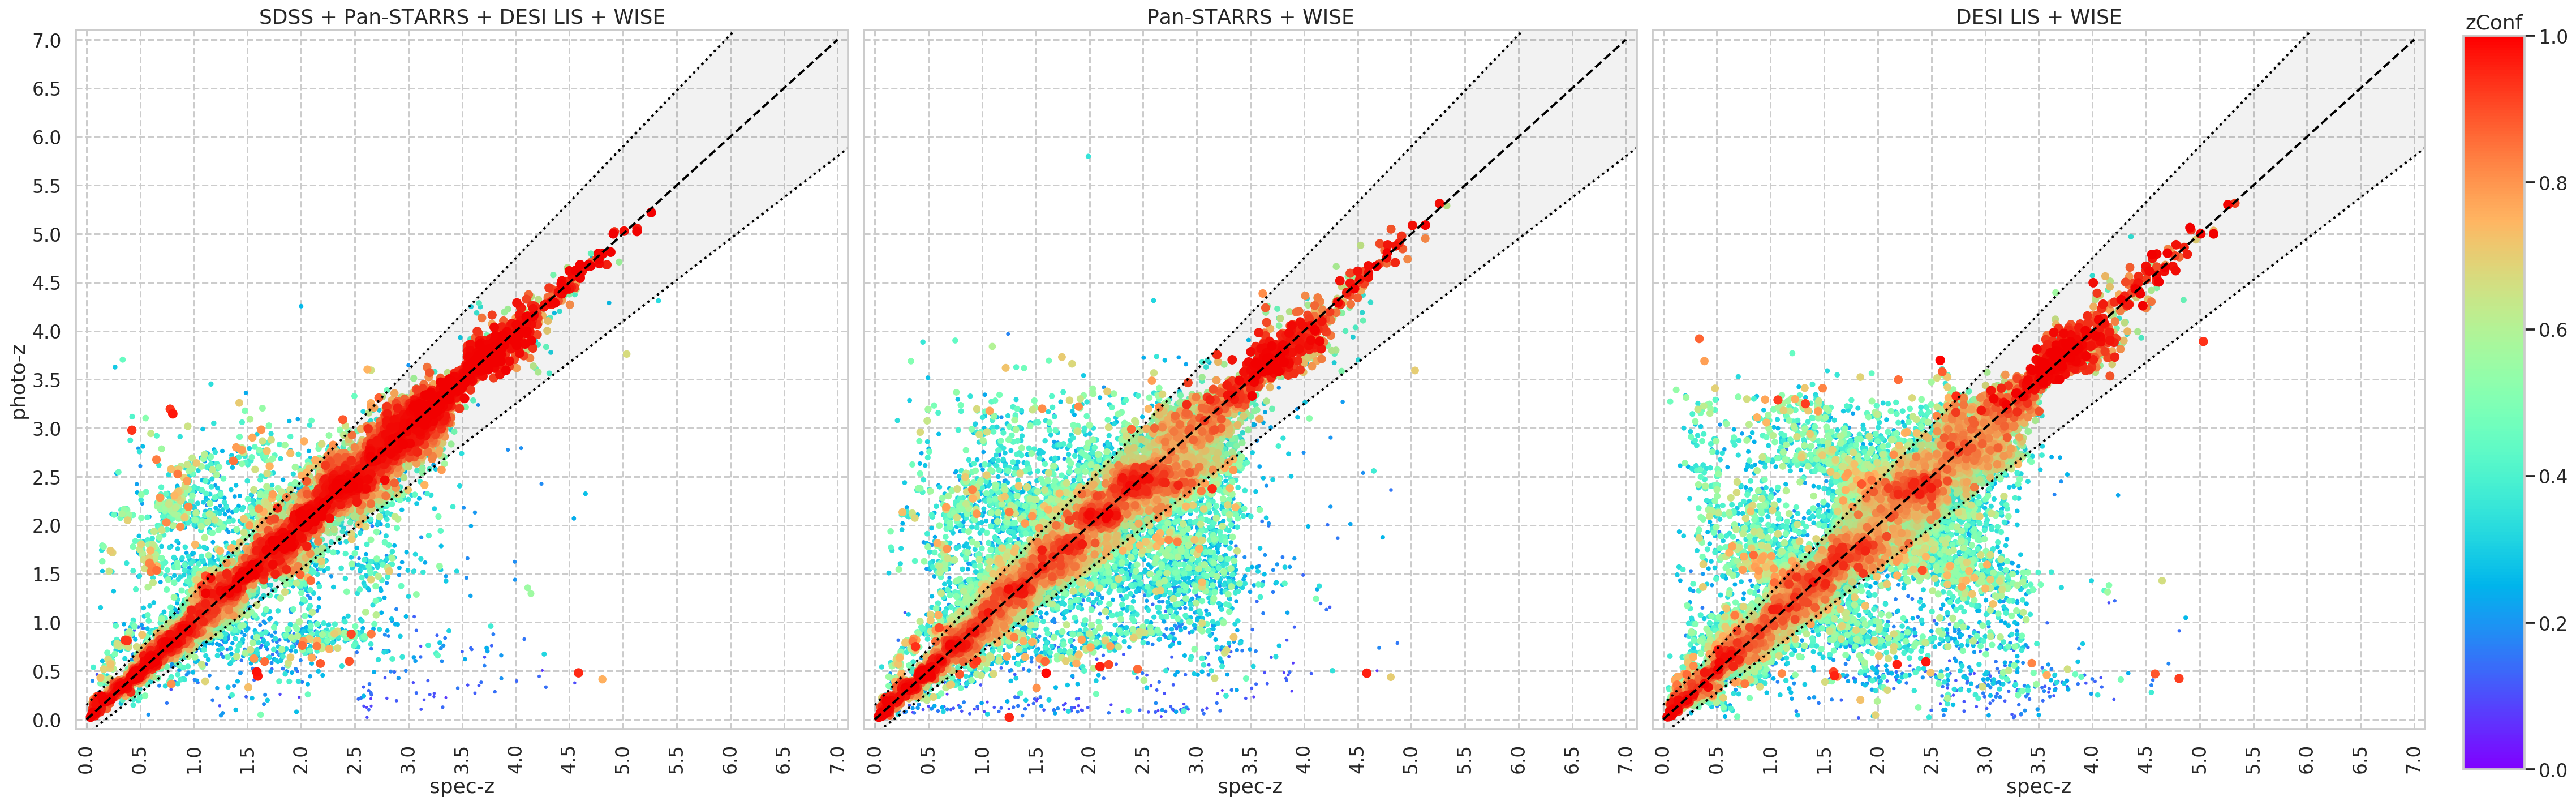
\includegraphics[width=0.99\linewidth]{images/scatterplots-dr16q-wo-train-sorted.png}
    \caption{Scatterplots of predictions on SDSS DR16 quasars test sample of three models (from left to right) -- \ref{model:spdw}, \ref{model:pw}, \ref{model:dw}. The abscissa axis shows the spectral redshift value, and the ordinate axis shows the photometric redshift prediction. The color and size of dots show the prediction reliability zConf \eqref{eq:zconf}. The gray area around the diagonal is the area of predictions that are not catastrophic emissions according to metric \eqref{eq:n015}.}
    \label{fig:scatter-dr16q_wo_train}
\end{figure*}

% \begin{figure*}
%     \centering
%     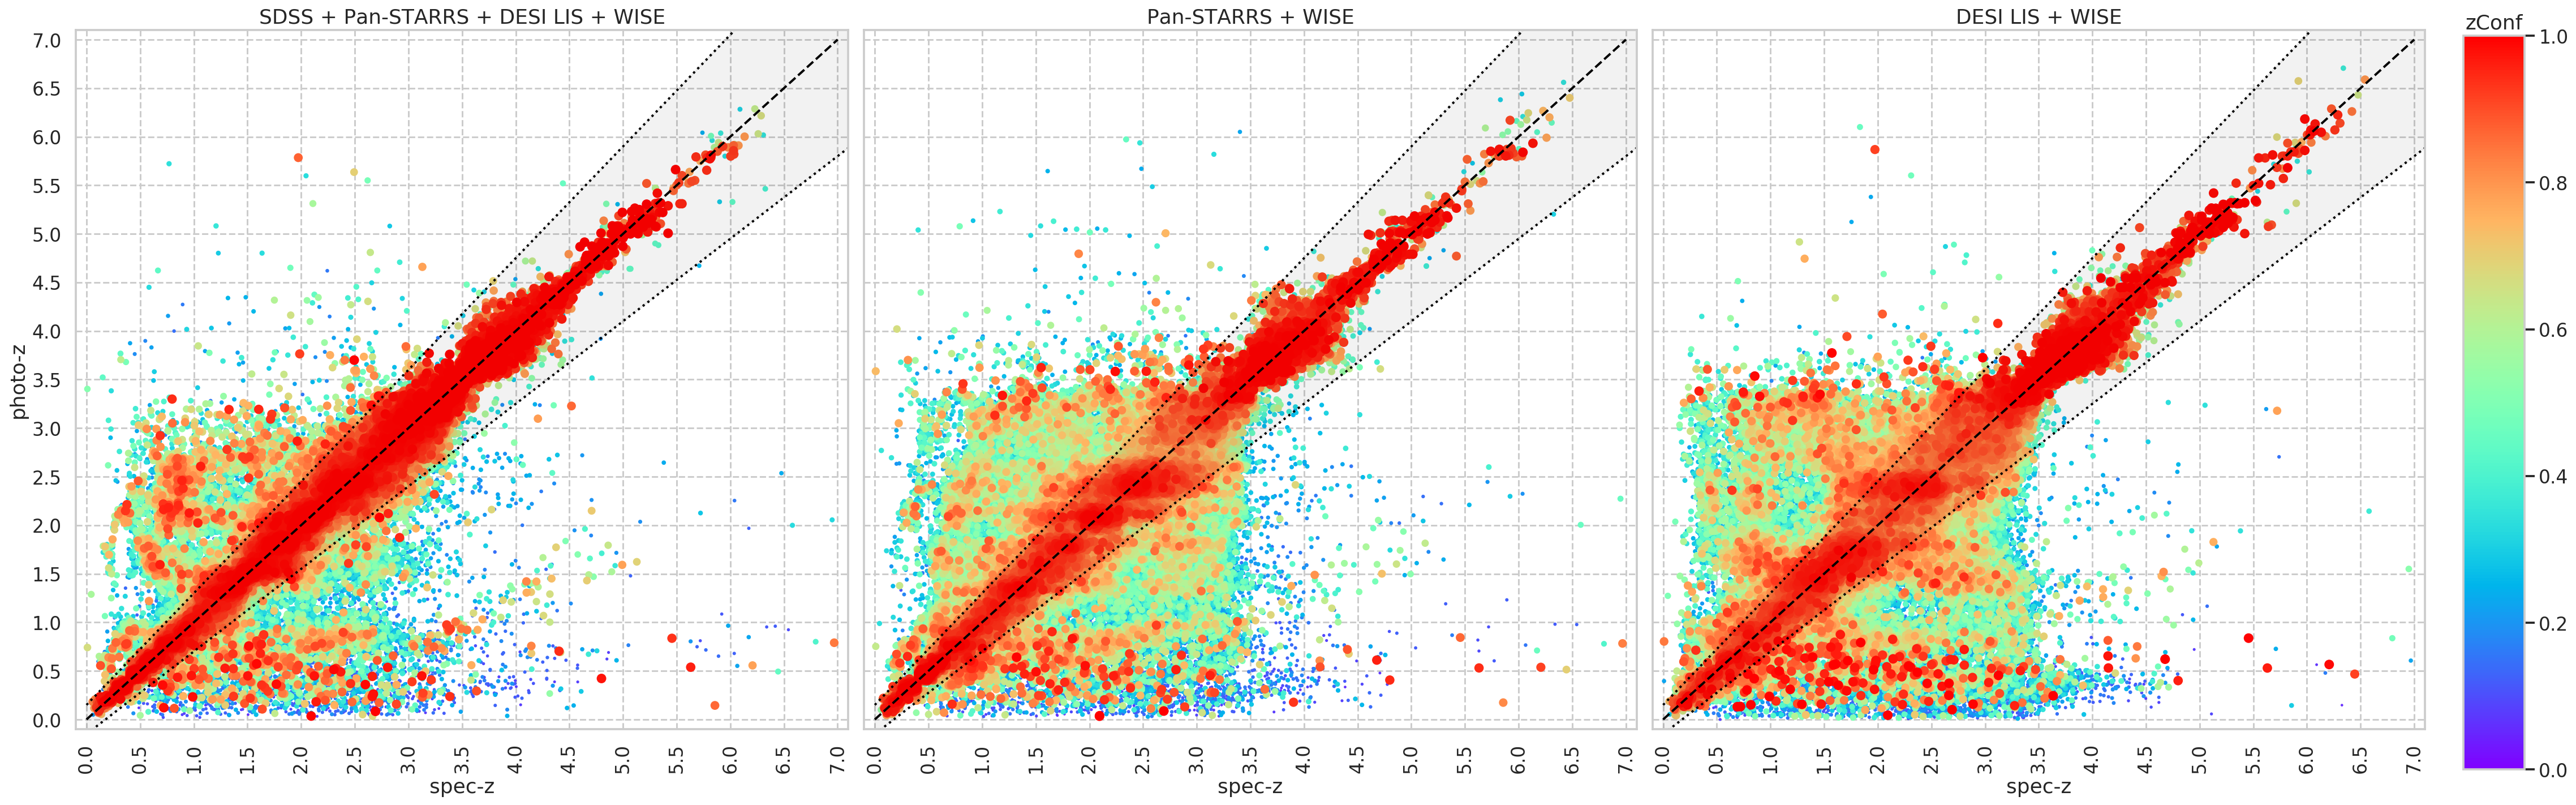
\includegraphics[width=0.9\linewidth]{images/scatterplots-cv2-qso-sorted.png}
%     \caption{Scatterplots of cross-validation predictions of quasars of three models (from left to right) -- \ref{model:spdw}, \ref{model:pw}, \ref{model:dw}. The abscissa axis shows the spectral redshift value, and the ordinate axis shows the photometric redshift prediction. The color and size of dots show the prediction reliability zConf \eqref{eq:zconf}. The gray area around the diagonal is the area of predictions that are not catastrophic emissions according to metric \eqref{eq:n015}.}
%     \label{fig:scatter-cv2-qso}
% \end{figure*}

\begin{figure*}
    \centering
    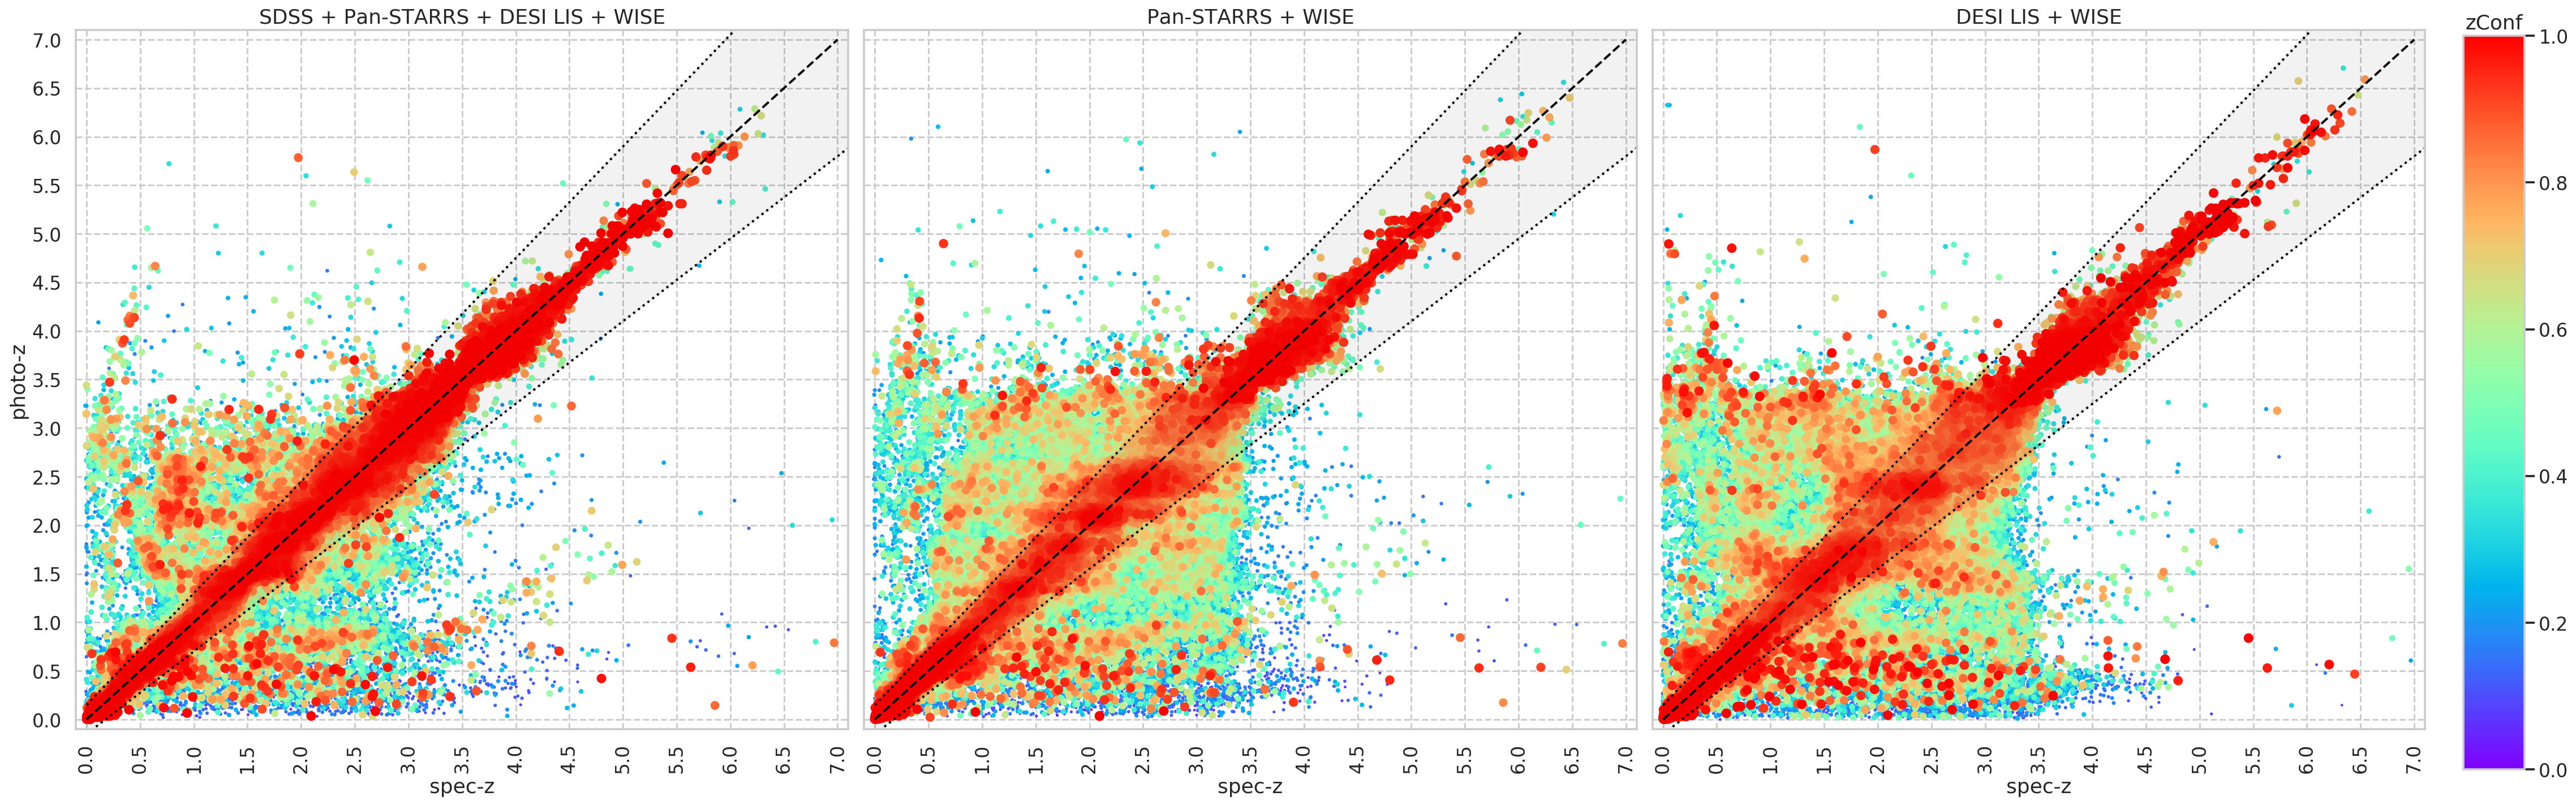
\includegraphics[width=0.99\linewidth]{images/scatterplots-cv2-total-sorted.png}
    \caption{Scatterplots of cross-validation predictions of galaxies and quasars of three models (from left to right) -- \ref{model:spdw}, \ref{model:pw}, \ref{model:dw}. The abscissa axis shows the spectral redshift value, and the ordinate axis shows the photometric redshift prediction. The color and size of dots show the prediction reliability zConf \eqref{eq:zconf}. The gray area around the diagonal is the area of predictions that are not catastrophic emissions according to metric \eqref{eq:n015}.}
    \label{fig:scatter-cv2-total}
\end{figure*}

На рис. \ref{fig:metrics-cv2-total} и \ref{fig:metrics-dr16q} справа приведены графики зависимости метрик качества точечных прогнозов $NMAD$ \eqref{eq:nmad} и $n_{>0.15}$ \eqref{eq:n015} от значения оптической AB-величины в фильтре $z$ для представленных пяти моделей на кросс-валидации и тестовой выборке квазаров DR16q, соответственно. Наблюдается монотонная зависимость от яркости источника в оптике на всех выборках. На кросс валидации (галактики и квазары) все модели показывают точность значительно выше более ярких источниках ($z_{mag} < 20$), чем на слабых сточниках ($z_{mag} > 21$). Точность может отличаться в 2-3 раза (например, в таблице \ref{tab:total_metrics_table}, где приведены метрики в пяти интервалах по spec-z и по $z_{mag}$: на кросс-валидации модель на всем небе \ref{model:pw} показывает значения метрик $NMAD, n_{>0.15} = 0.043, 0.079$ на объектах $19 \leq z_{mag} < 20$ и $NMAD, n_{>0.15} = 0.089, 0.213$ на объектах $21 \leq z_{mag} < 23$, а наиболее точная модель \ref{model:spdw} -- $NMAD, n_{>0.15} = 0.026, 0.034$ и $NMAD, n_{>0.15} = 0.048, 0.093$, соответственно.

На тестовой выборке квазаров DR16q наблюдается в целом та же зависимость, но, ввиду отсутствия объектов типа галактика в выборке, значения метрик ухудшаются на наиболее ярких квазарах $z_{mag} < 19$, что можно видеть на рис. \ref{fig:metrics-cv2-total} и \ref{fig:metrics-dr16q} (все модели показывают точность не лучше $NMAD, n>0.15 = 0.02, 0.02$). При этом все модели показывают точность не хуже $NMAD, n>0.15 = 0.04, 0.10$ кроме модели \ref{model:dw}, которая показывает точность в среднем $NMAD, n>0.15 = 0.07, 0.15$.

Добавление в модель признаков DESI LIS так же значительно улучшает точность моделей на слабых источниках (см. модели \ref{model:pw} и \ref{model:pdw} и модели \ref{model:spw} и \ref{model:spdw} на рис \ref{fig:metrics-cv2-total} и \ref{fig:metrics-dr16q} и в таблице \ref{tab:total_metrics_table} для $21 < z_{mag} < 23$), при том модель \ref{model:dw} на основе только признаков DESI LIS и WISE превосходит по точности только модель \ref{model:pw} на основе только признаков Pan-STARRS, и только на наиболее слабых источниках (квазарах с $z_mag > 21.5$, см. рис. \ref{fig:metrics-dr16q}).

\clearpage
\subsubsection{Зависимость от класса объекта (QSO/GALAXY)}
\begin{figure*}
    \centering
    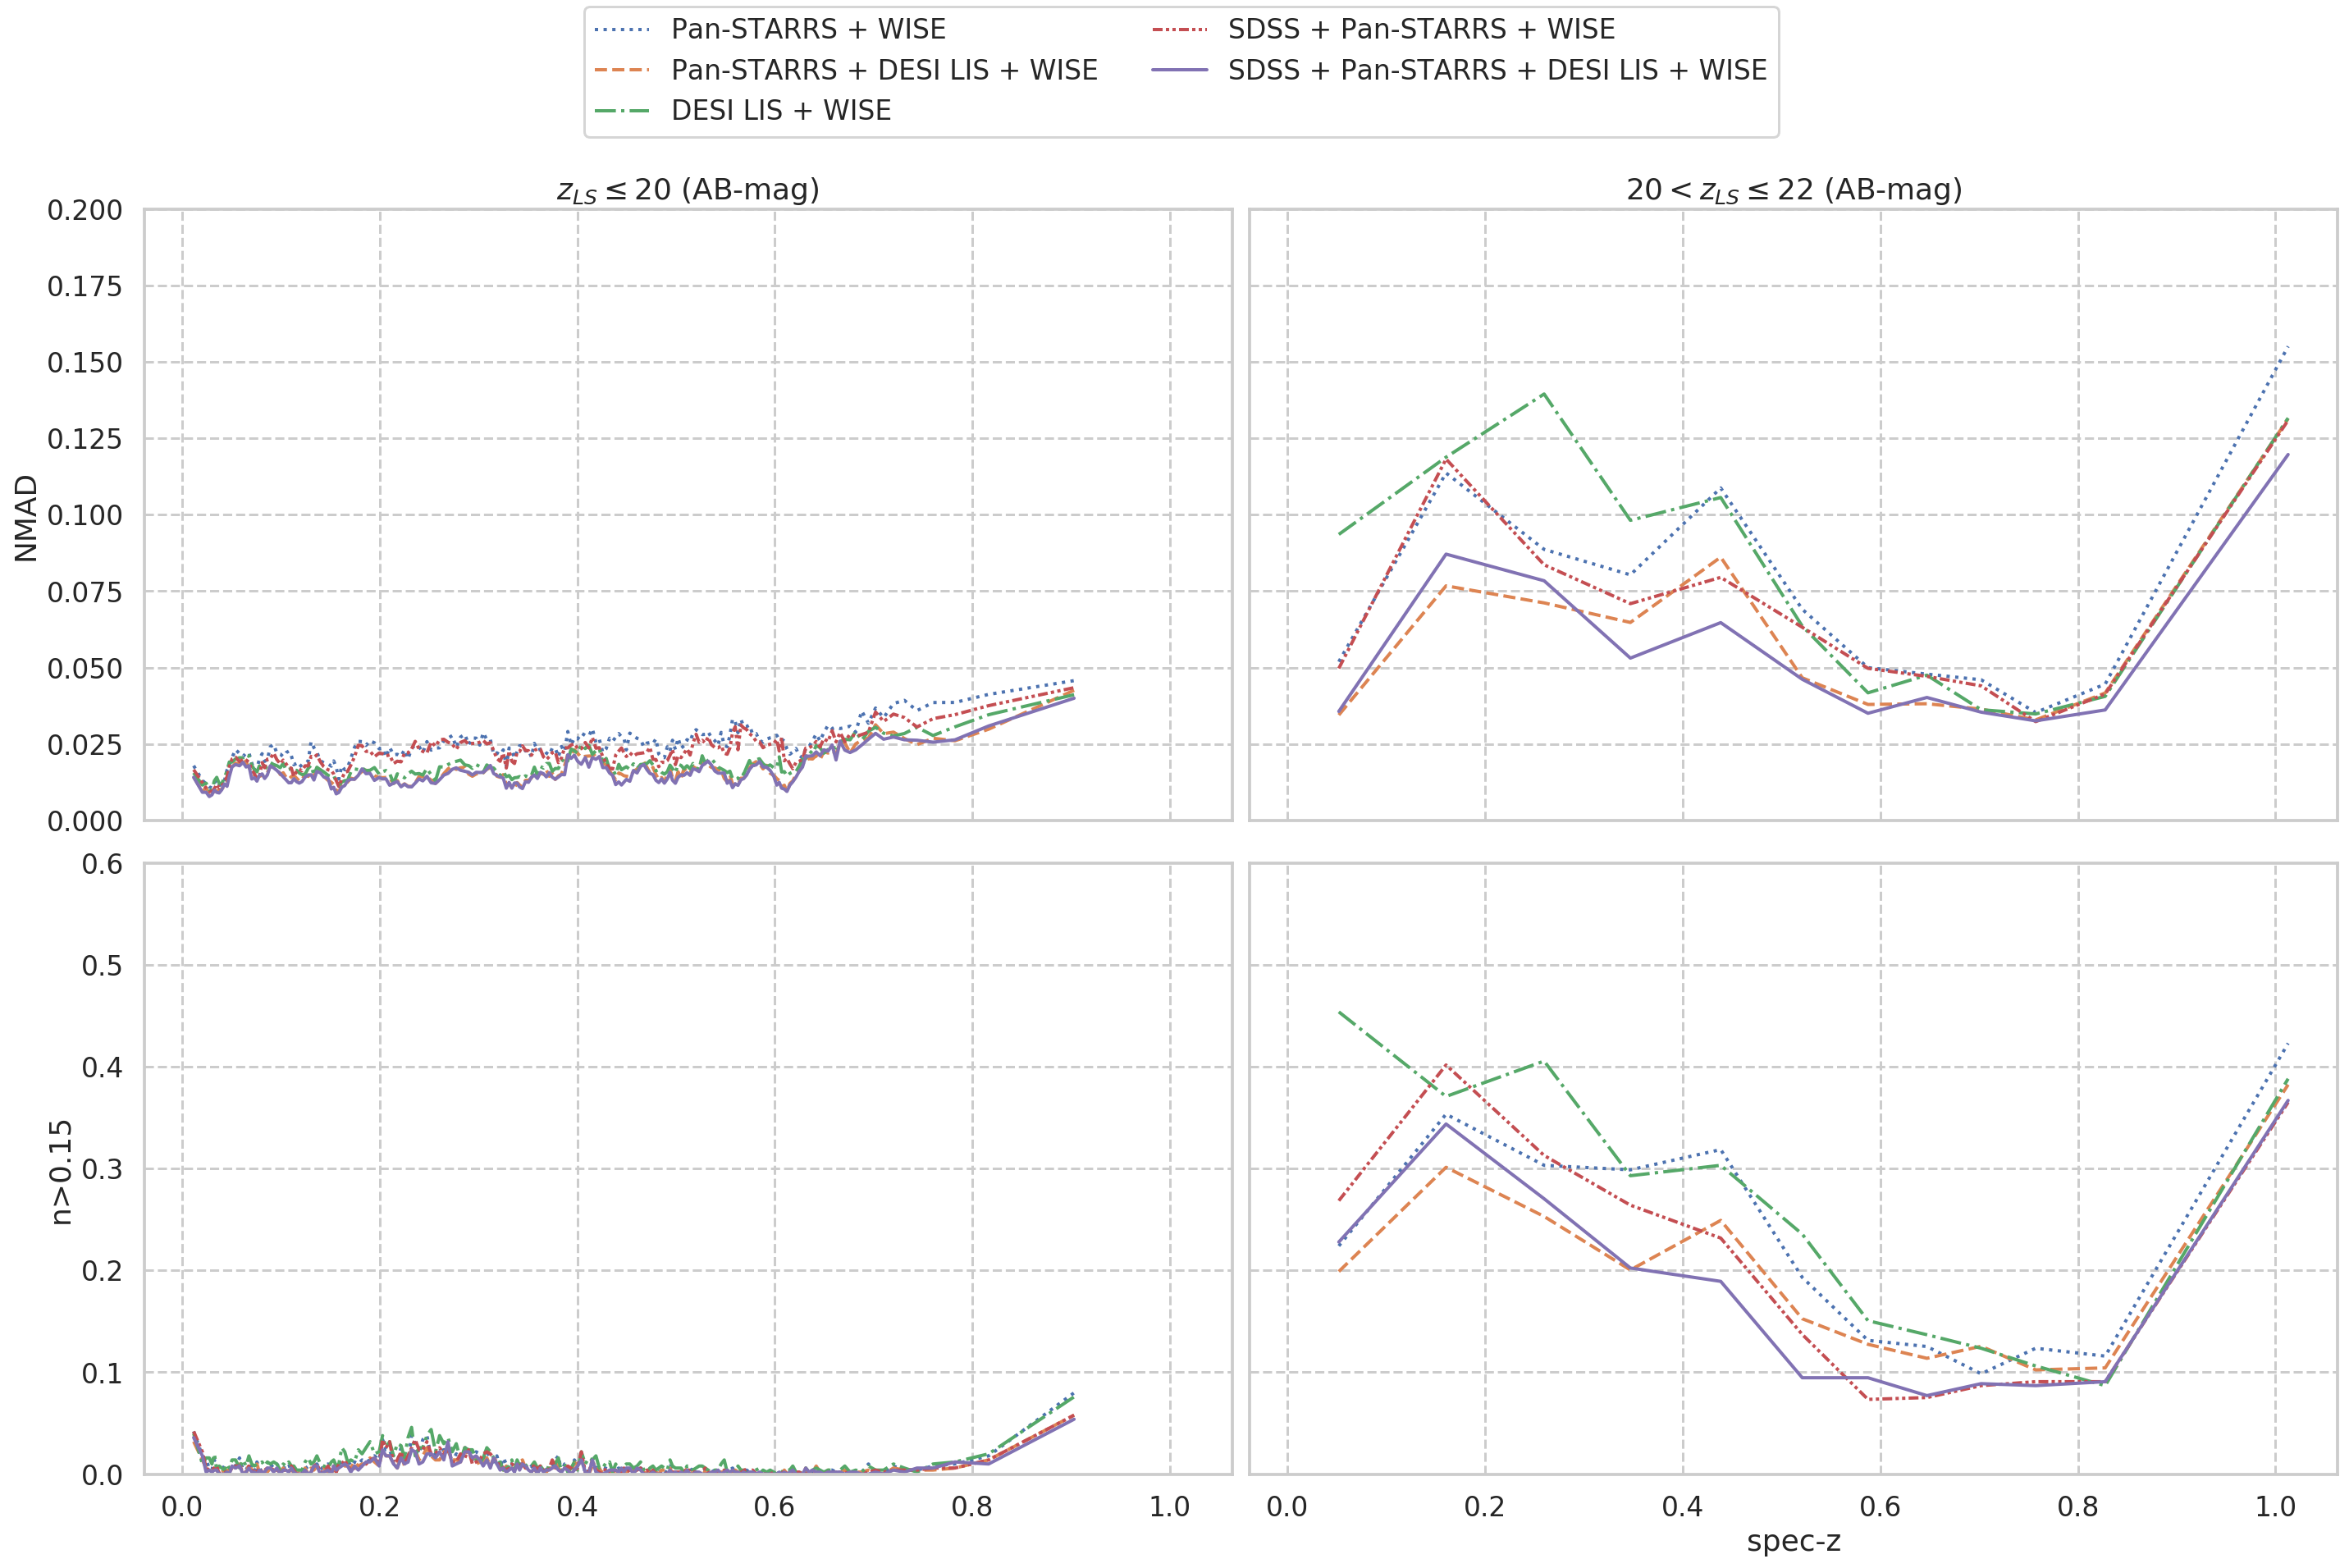
\includegraphics[width=0.99\linewidth]{images/class-galaxy-cv2.png}
    \caption{Метрики на ярких и слабых галактиках на кросс-валидации в зависимости от spec-z}
    \label{fig:class-galaxy-cv2}
\end{figure*}

\begin{figure*}
    \centering
    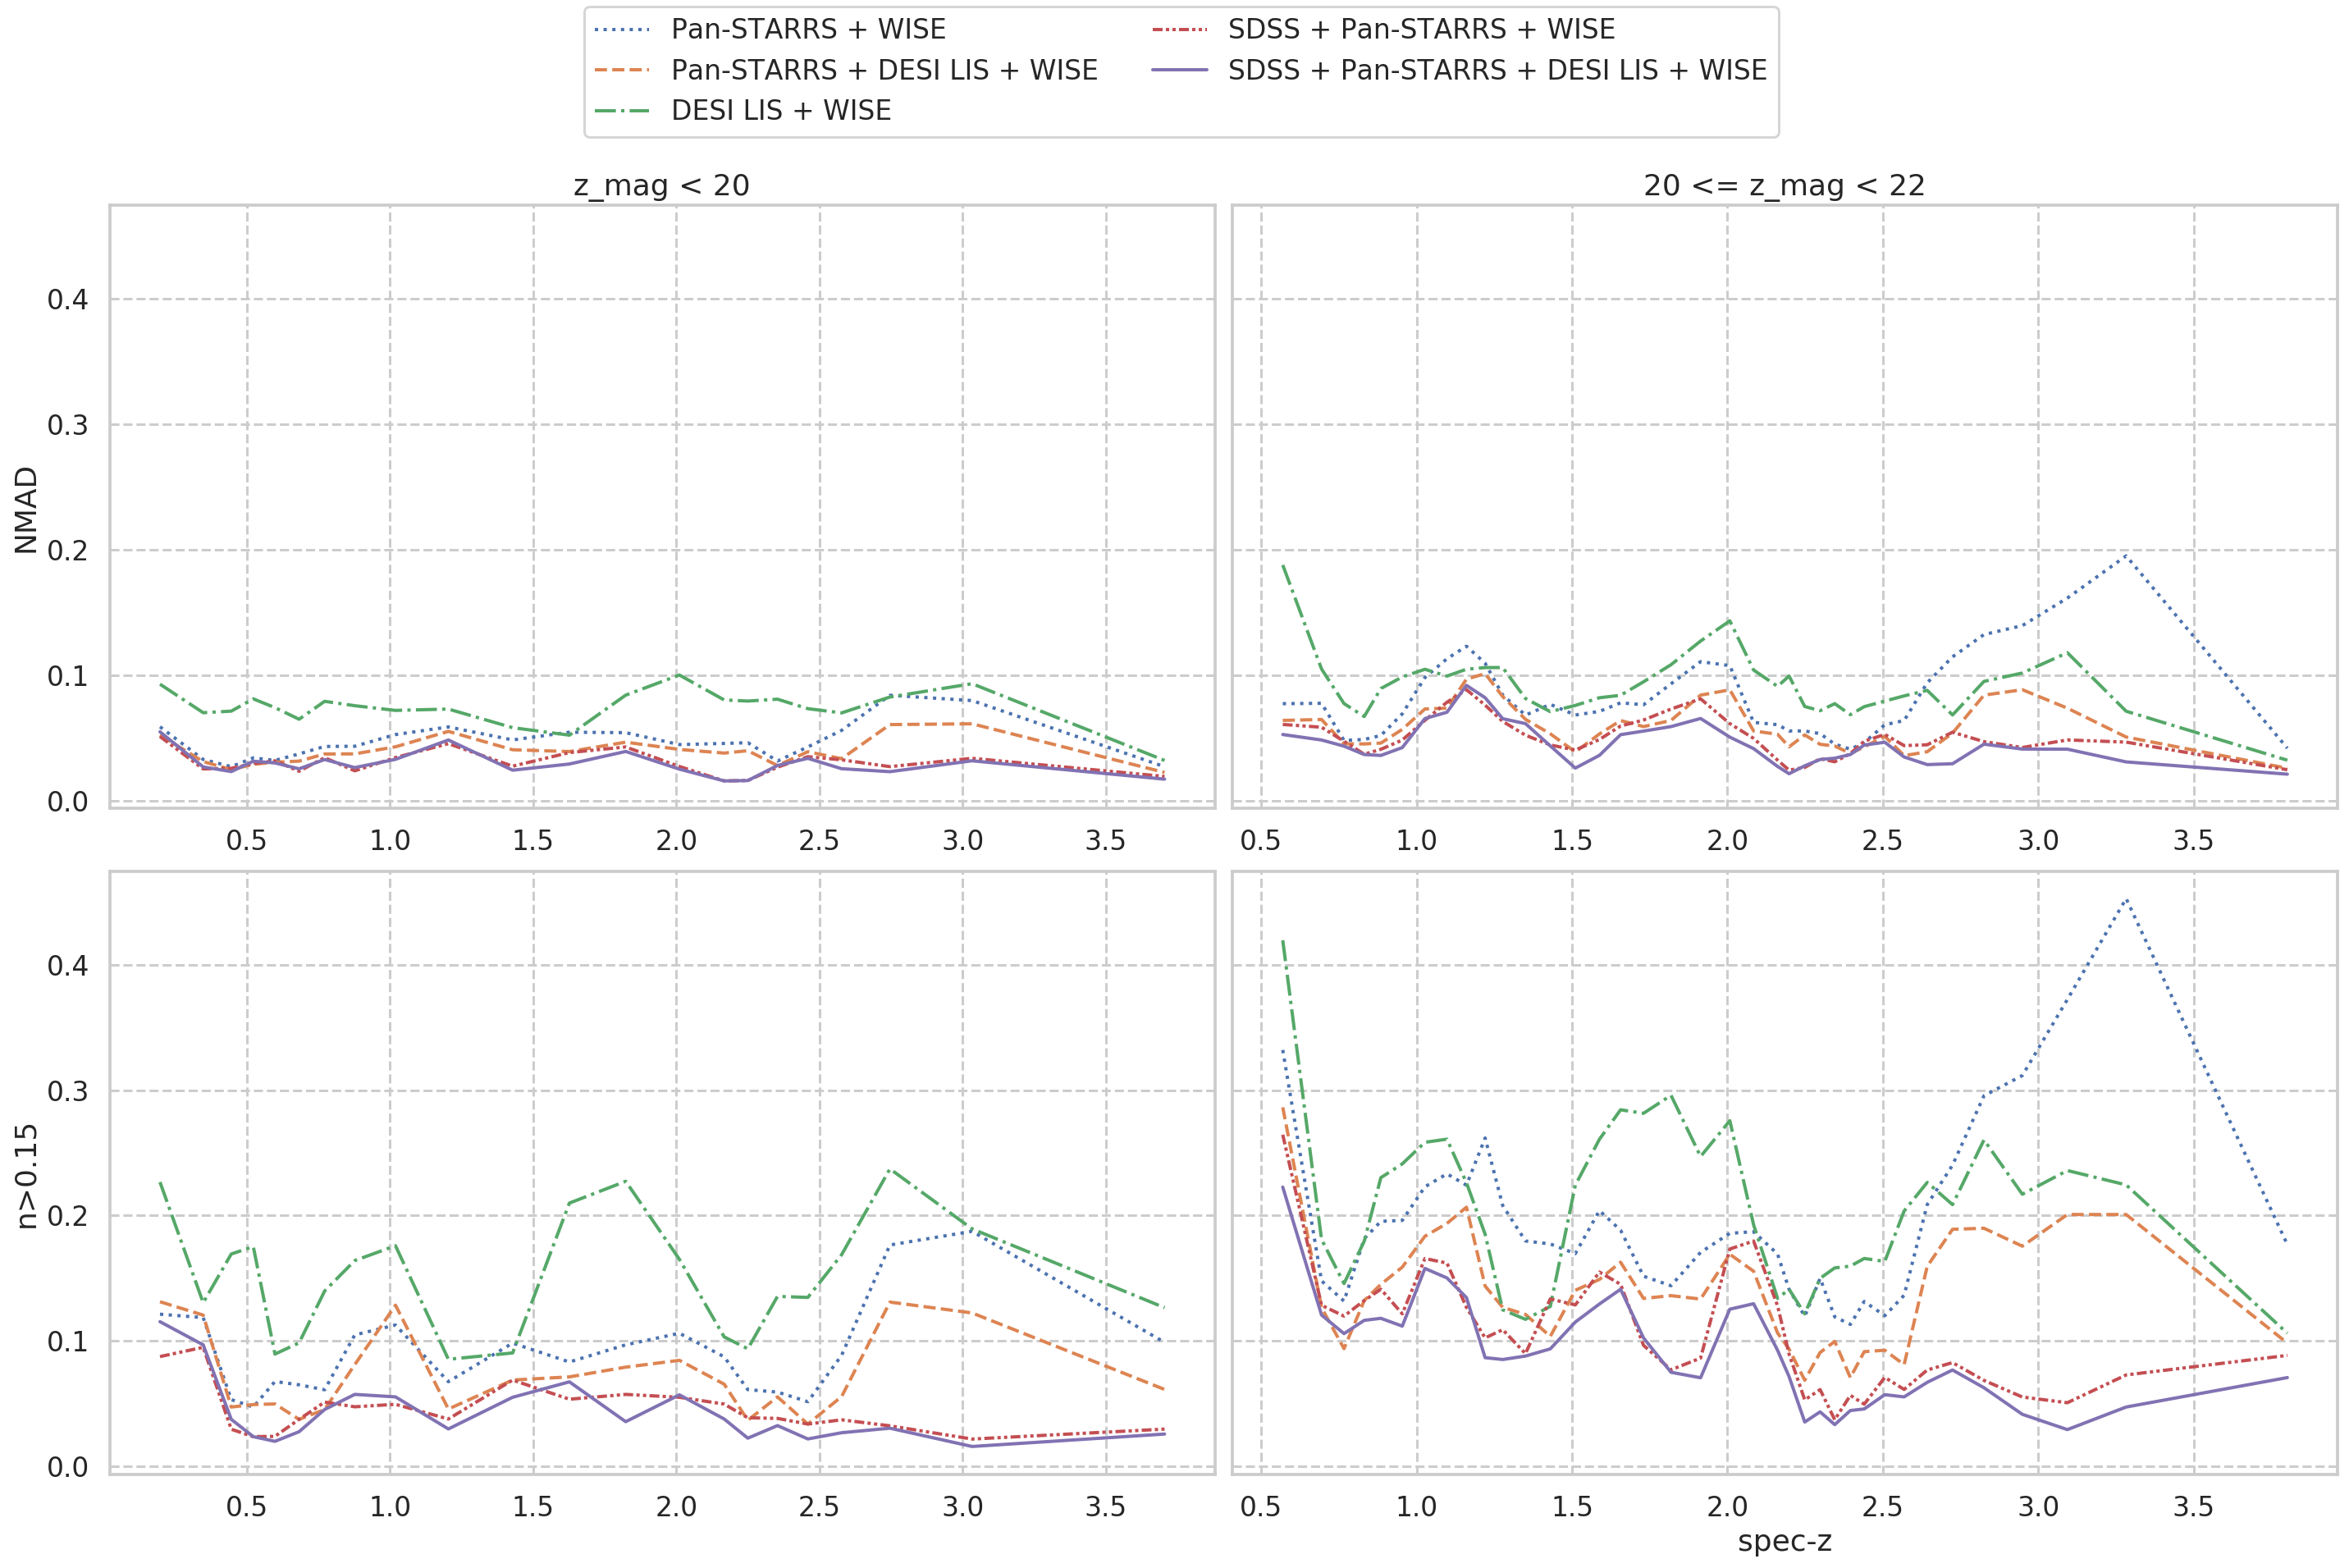
\includegraphics[width=0.99\linewidth]{images/class-qso-dr16q.png}
    \caption{Метрики на ярких и слабых квазарах DR16q в зависимости от spec-z}
    \label{fig:class-qso-dr16q}
\end{figure*}

%\begin{figure*}
%    \centering
%    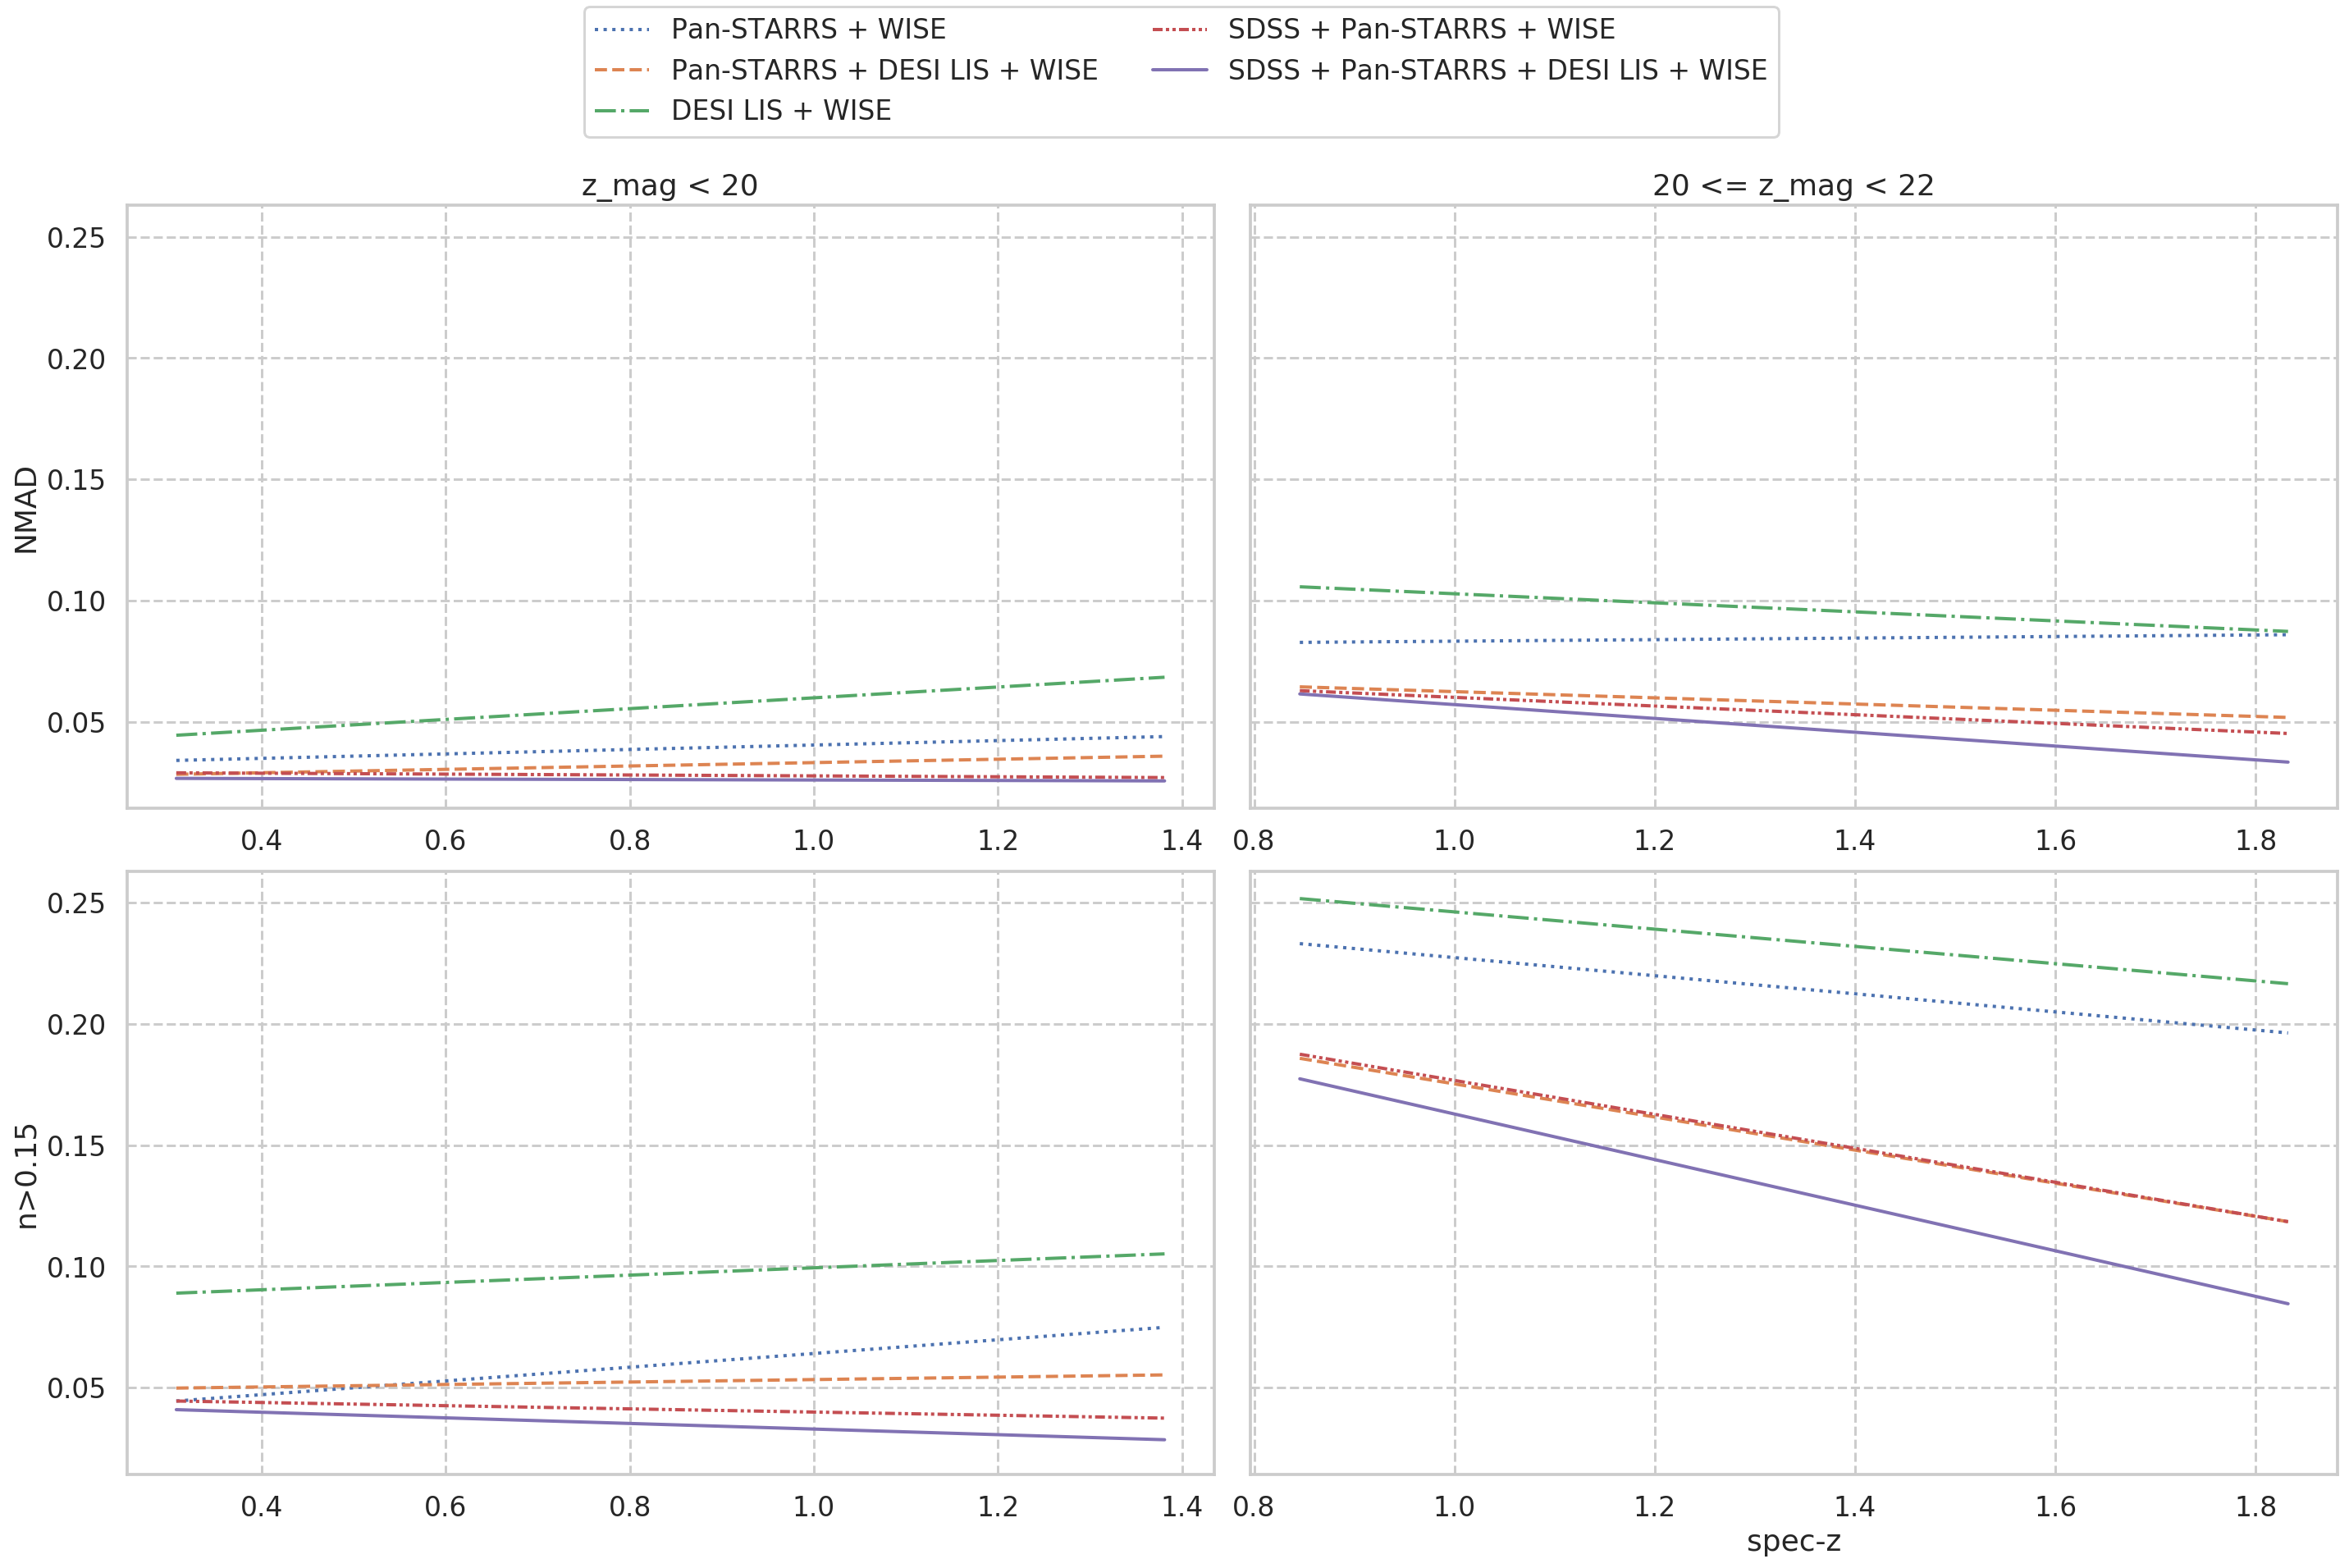
\includegraphics[width=0.99\linewidth]{images/class-xray-s82x.png}
%    \caption{Метрики на ярких и слабых рентгеновских источниках в зависимости от spec-z}
%    \label{fig:class-xray-s82x}
%\end{figure*}

\subsection{Отбор объектов по параметру уверенности прогноза (zConf)}

\begin{figure*}
    \centering
    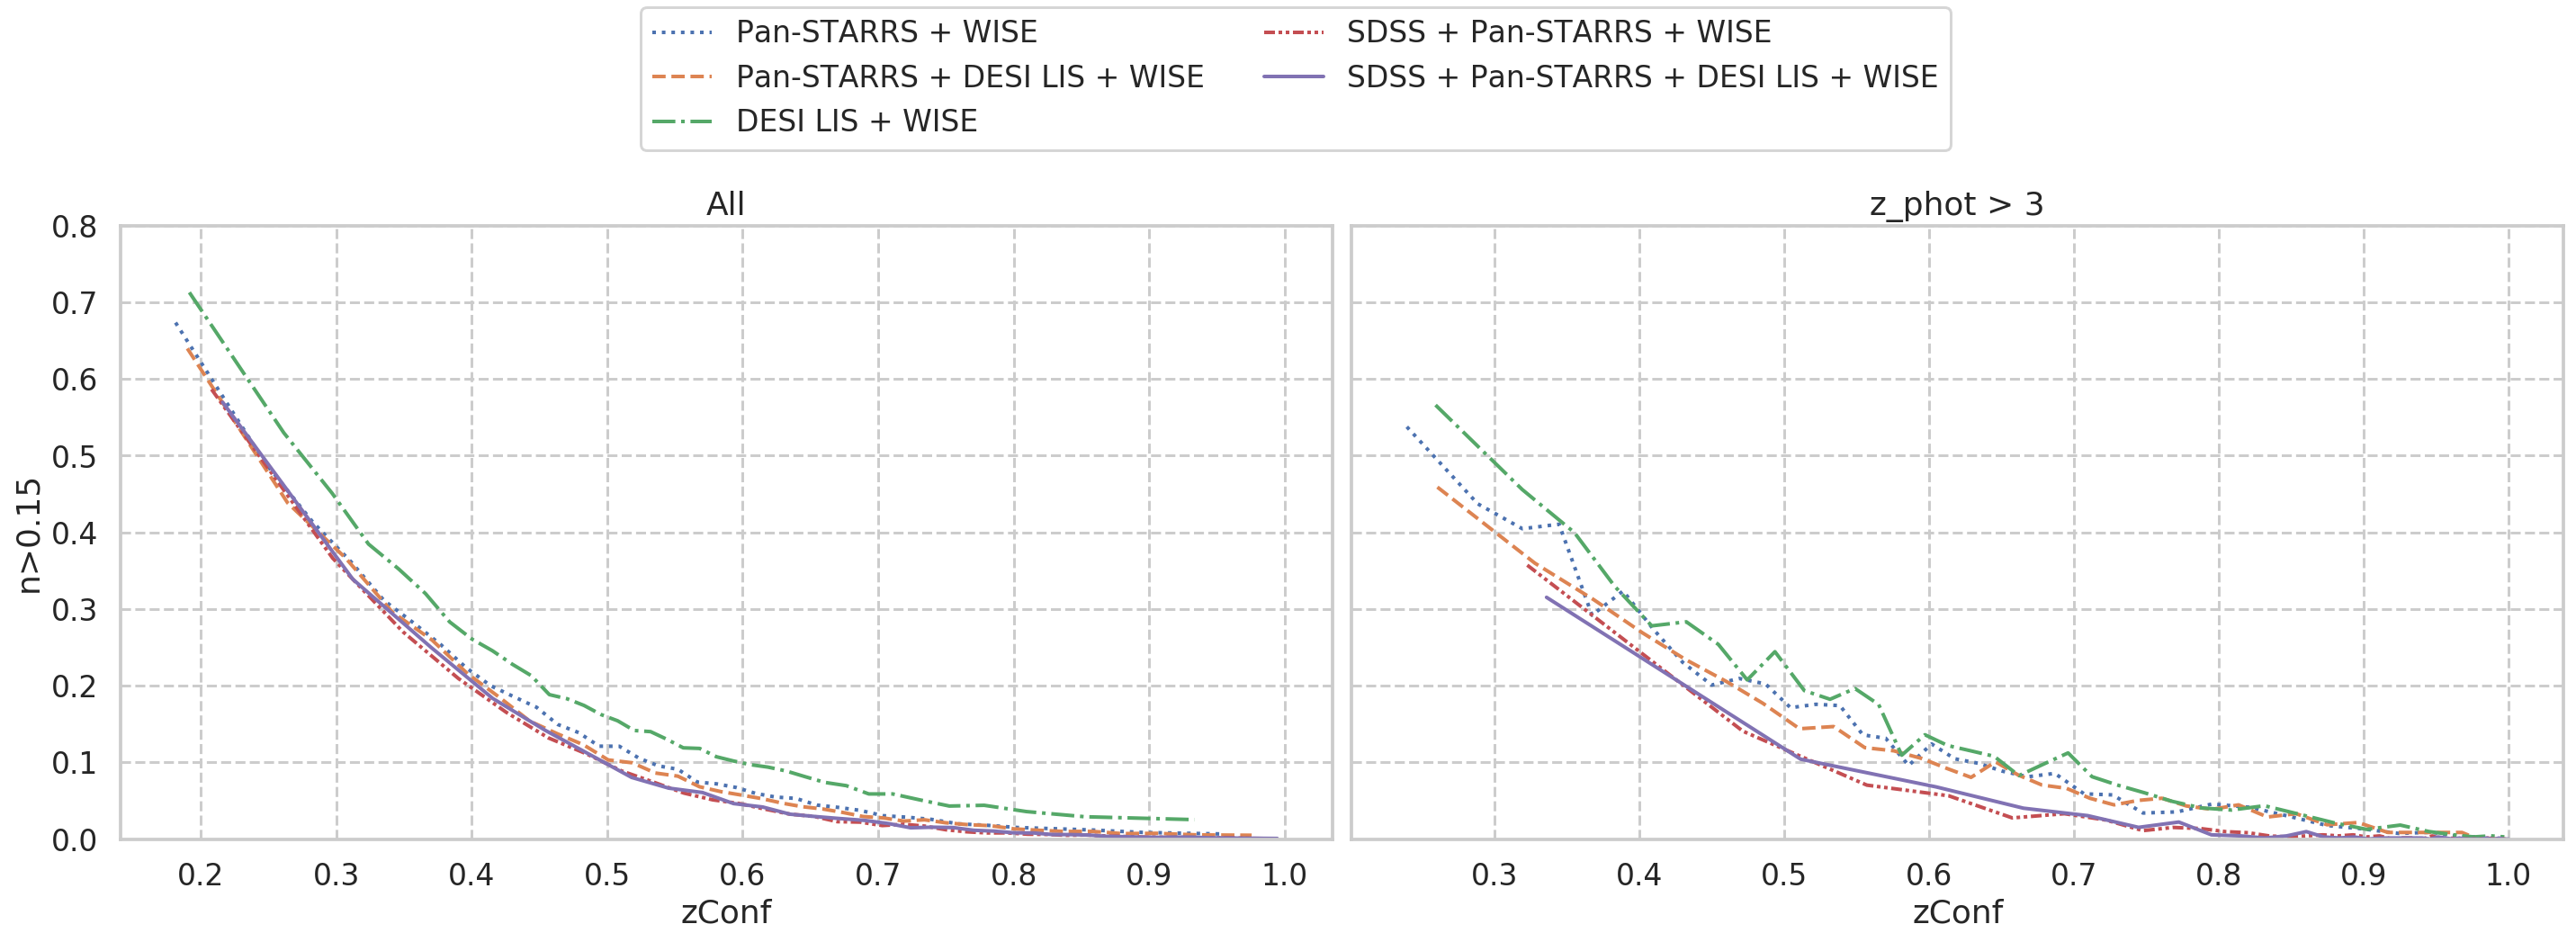
\includegraphics[width=0.99\linewidth]{images/metrics-by-zconf-cv2-qso.png}
    \caption{Метрики в зависимости от zConf на квазарах кросс-валидации}
    \label{fig:metrics-zconf-cv2}
\end{figure*}

\begin{figure*}
    \centering
    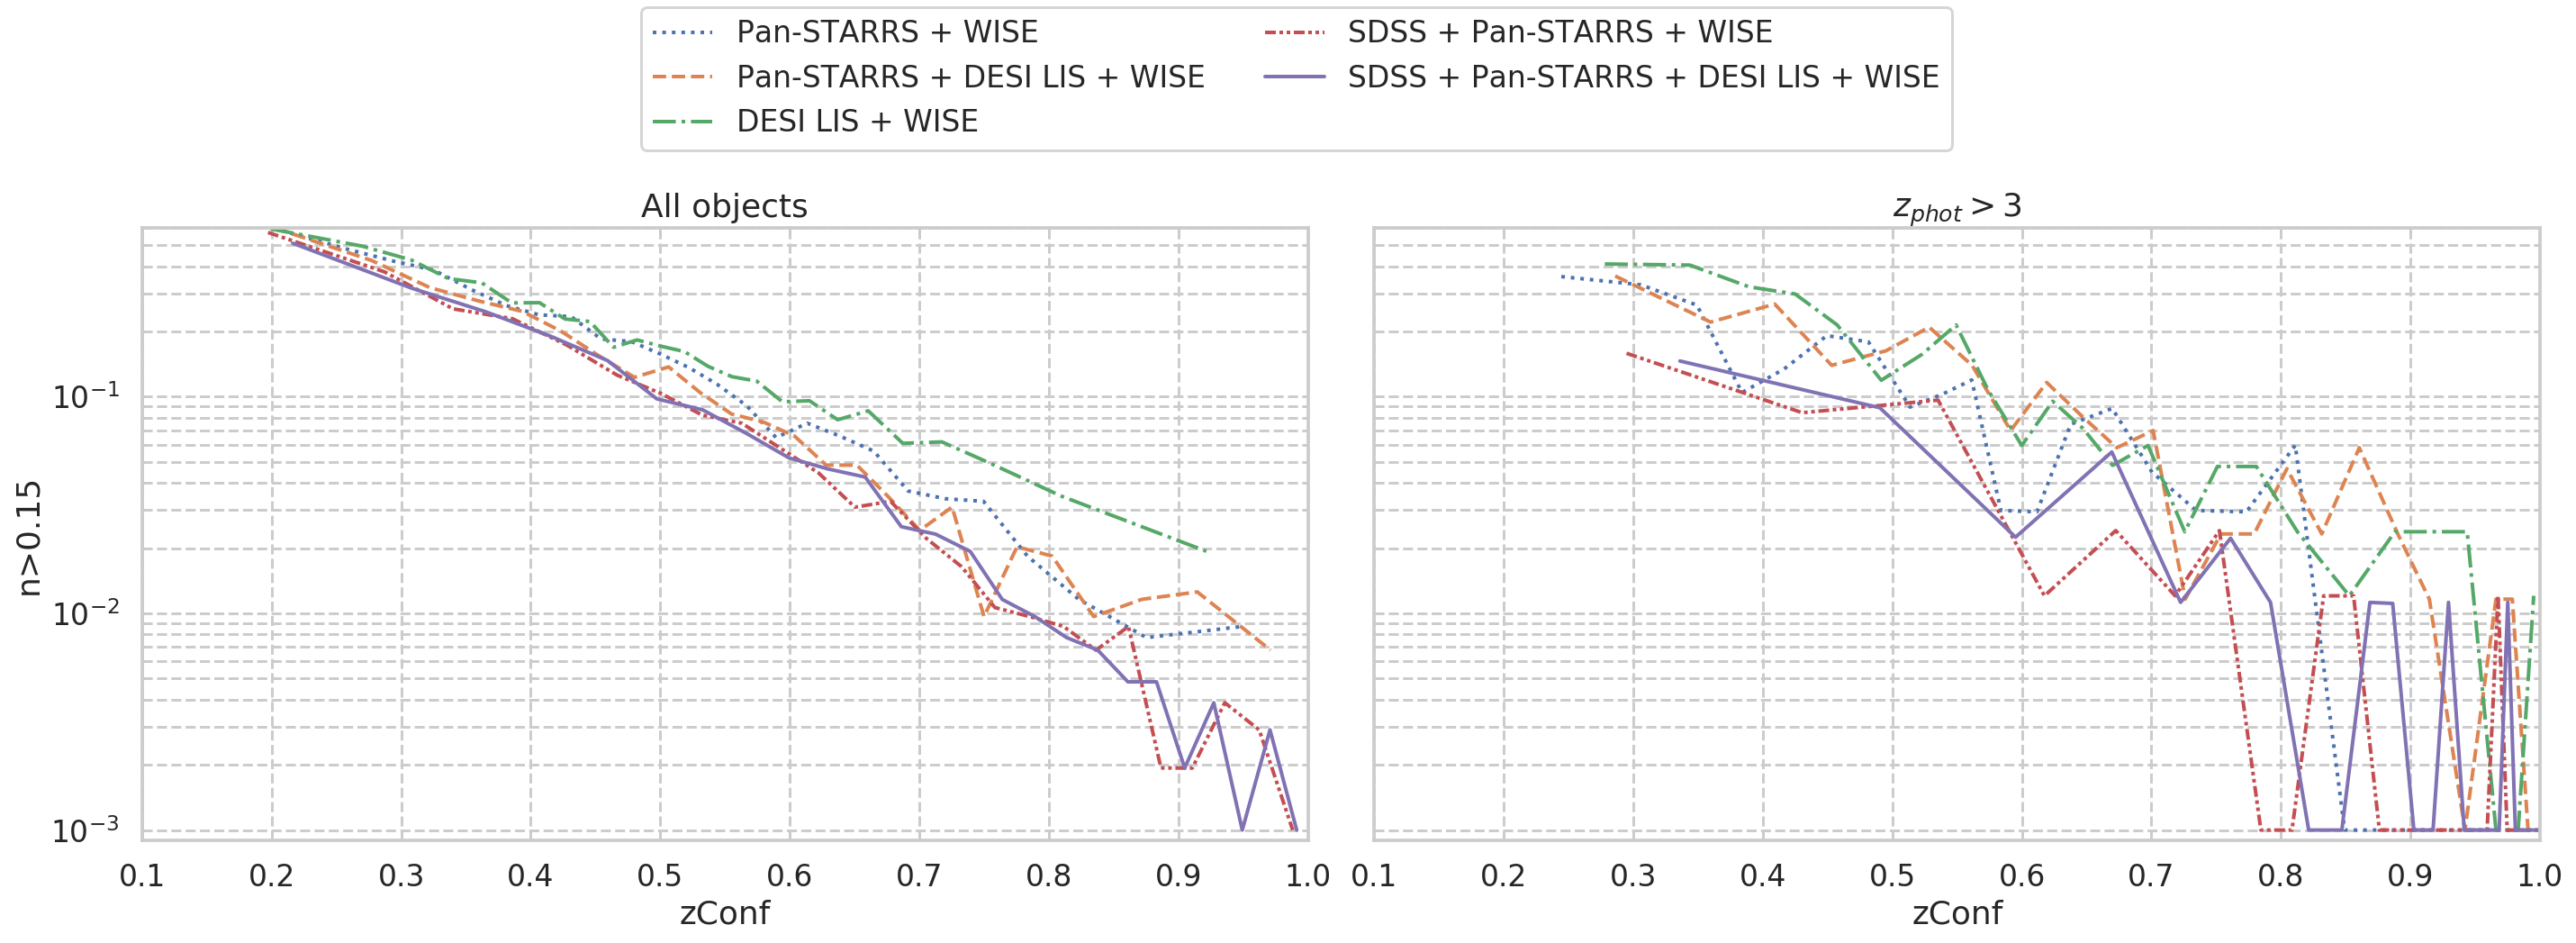
\includegraphics[width=0.99\linewidth]{images/metrics-by-zconf-dr16q.png}
    \caption{Метрики в зависимости от zConf на DR16q}
    \label{fig:metrics-zconf-cv2}
\end{figure*}

\begin{figure*}
    \centering
    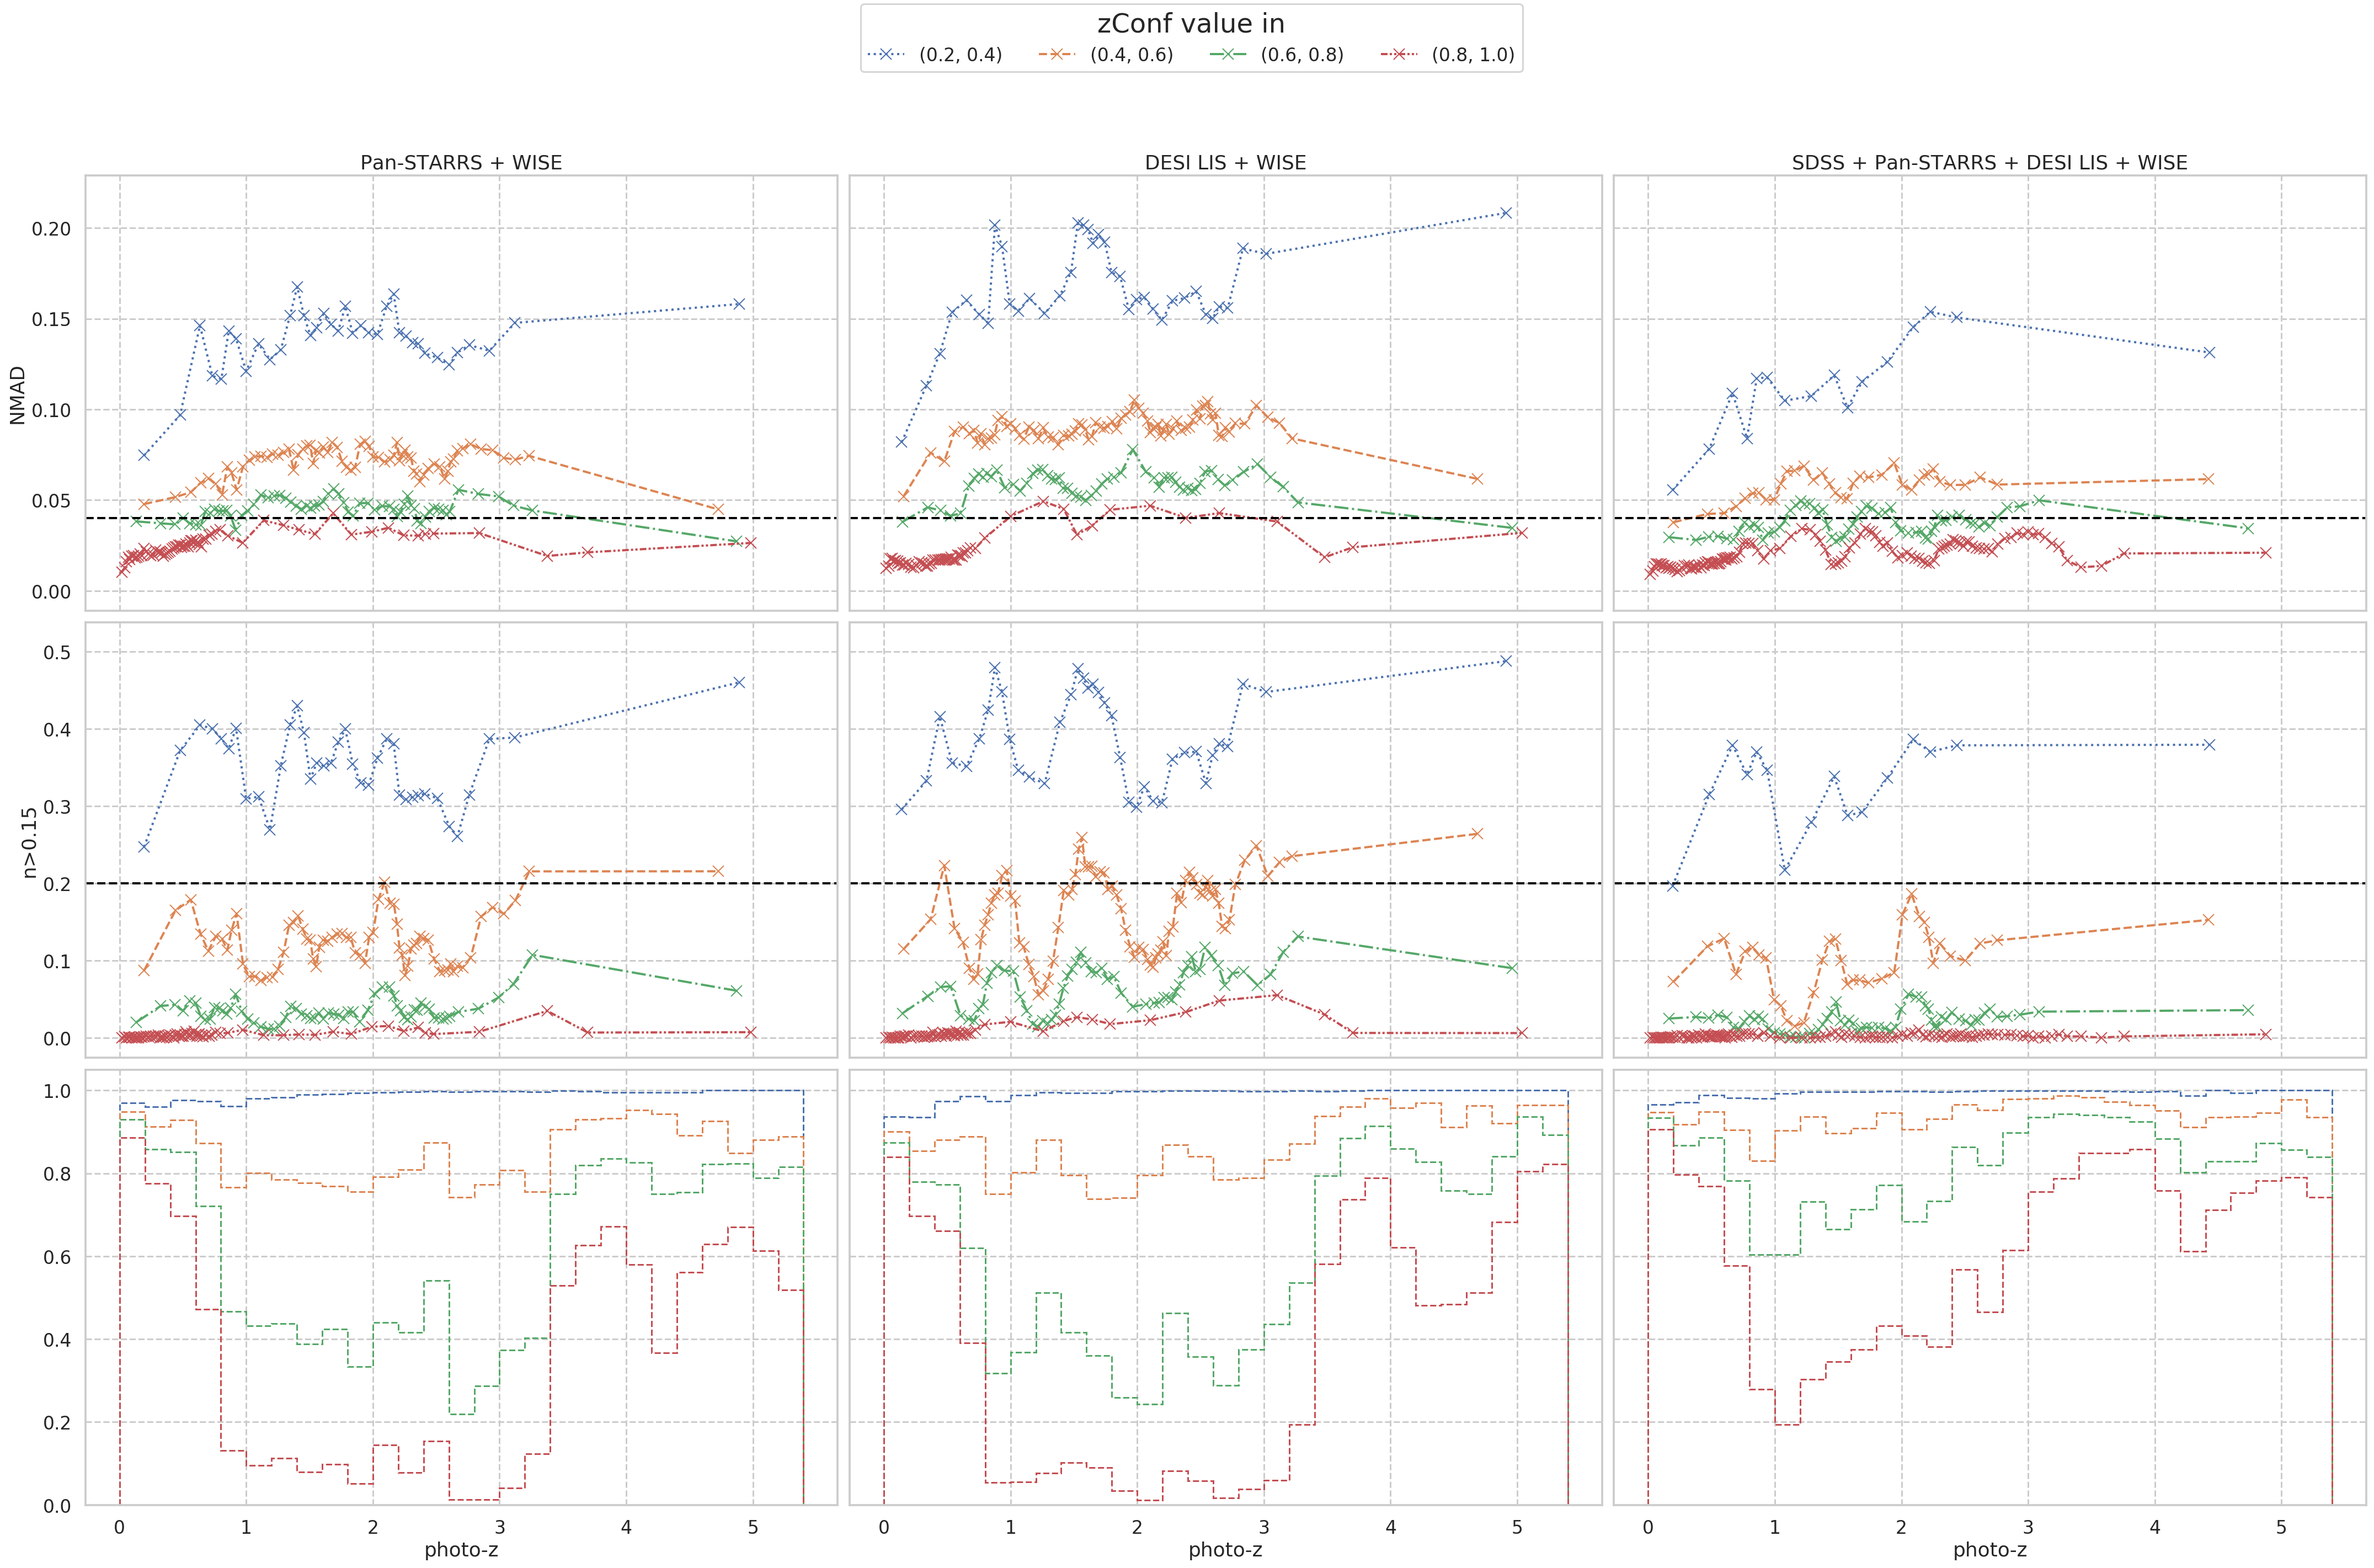
\includegraphics[width=0.99\linewidth]{images/metrics-zconf-cv2.png}
    \caption{Метрики в зависимости от zConf}
    \label{fig:metrics-zconf-cv2}
\end{figure*}

\begin{figure*}
    \centering
    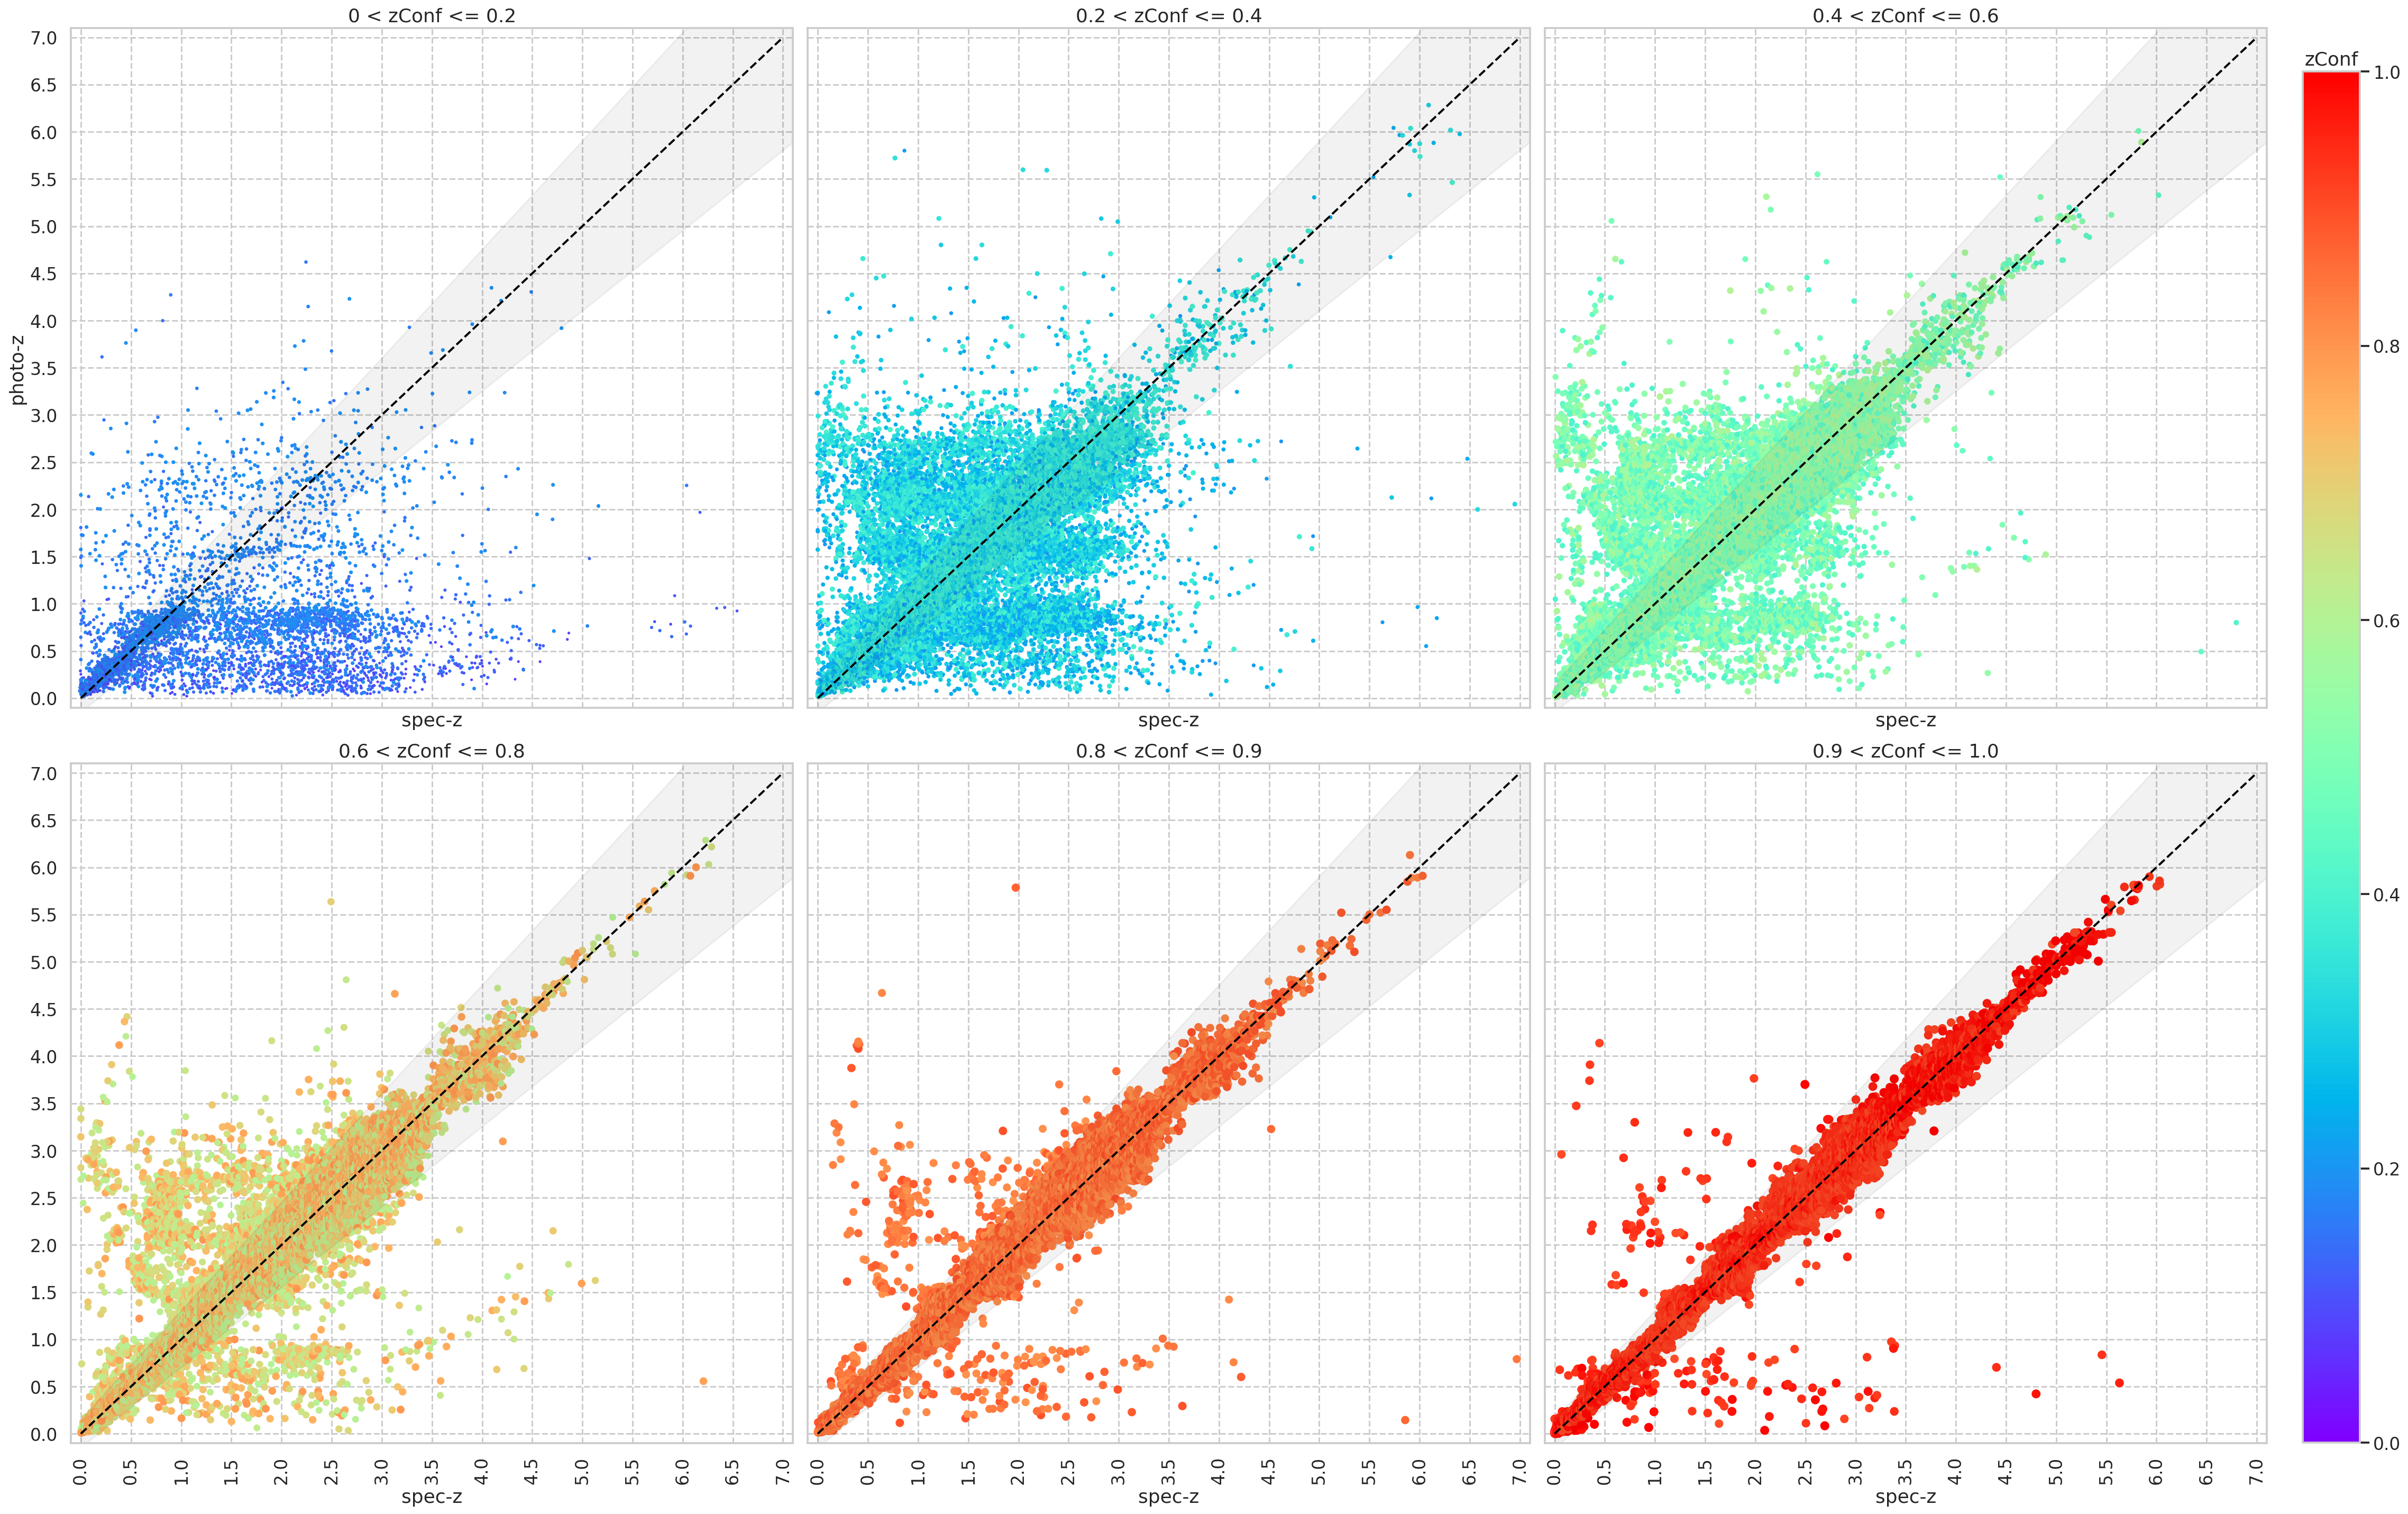
\includegraphics[width=0.99\linewidth]{images/zconf-scatterplot-35.png}
    \caption{Скаттерплоты в зависимости от zConf для модели \ref{model:spdw}}
    \label{fig:zconf-scatterplot-35}
\end{figure*}

\begin{figure*}
    \centering
    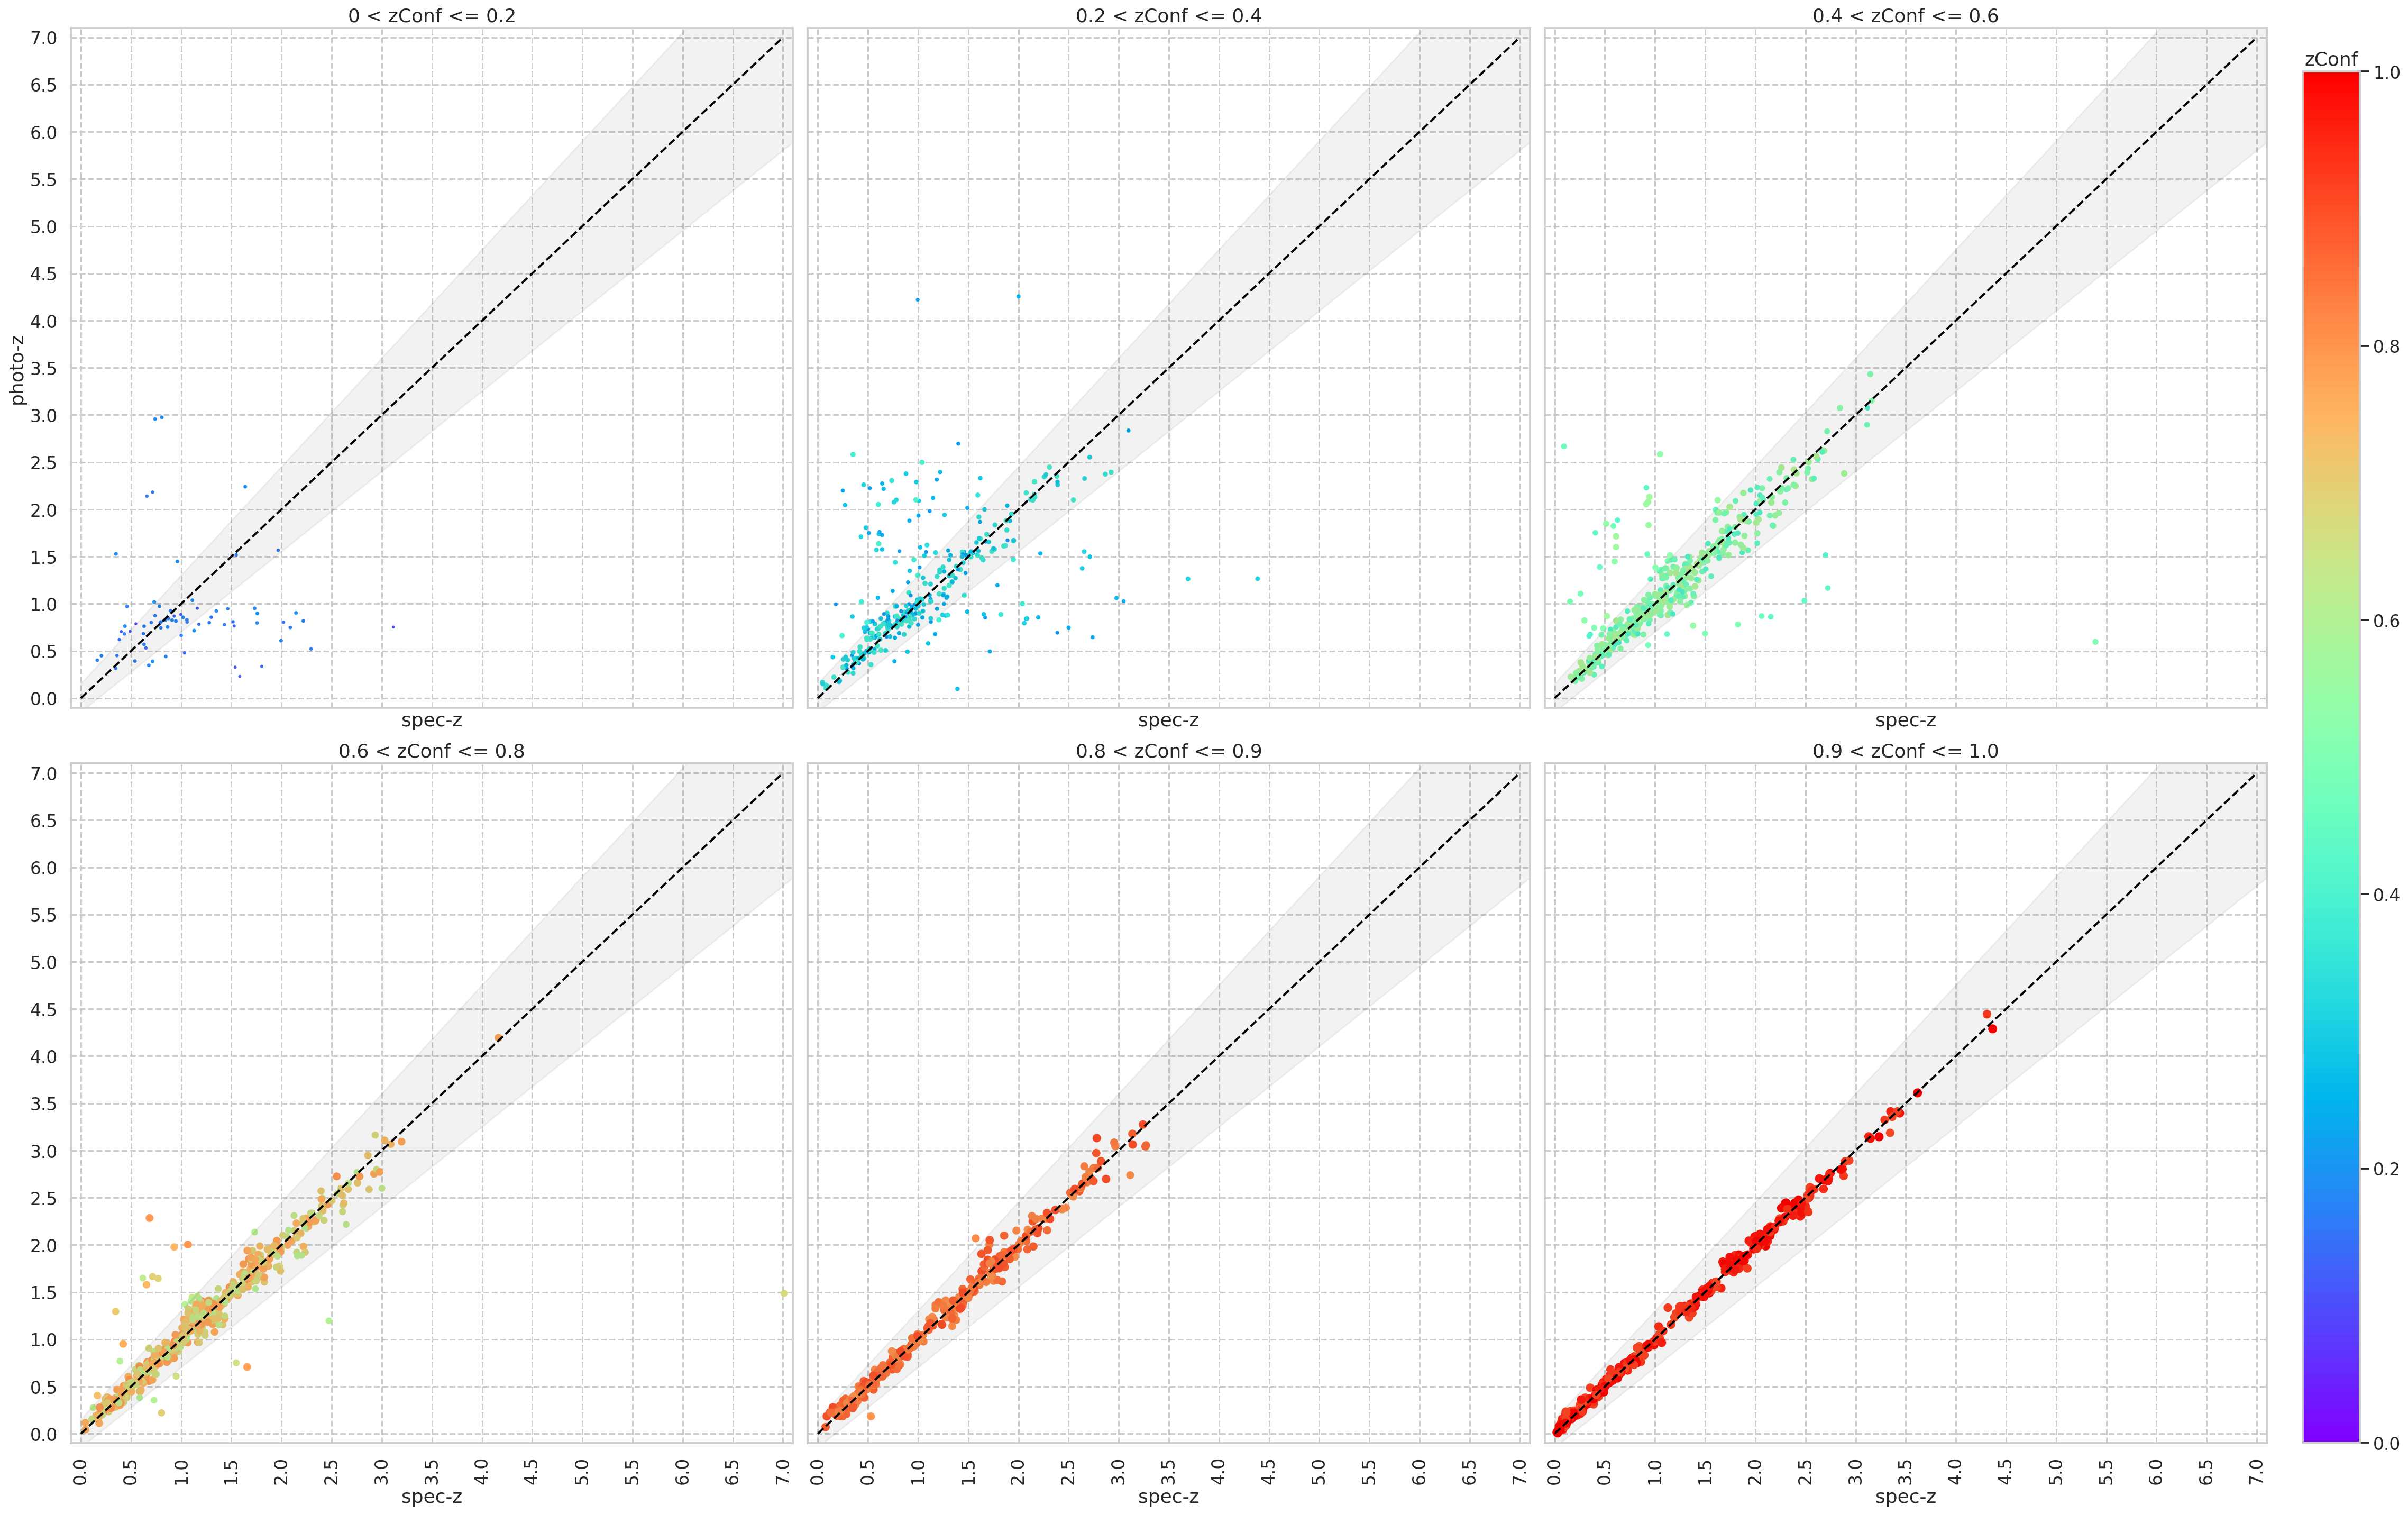
\includegraphics[width=0.99\linewidth]{images/zconf-scatterplot-35-s82x.png}
    \caption{Скаттерплоты в зависимости от zConf для модели \ref{model:spdw} на S82X}
    \label{fig:zconf-scatterplot-35}
\end{figure*}

\subsection{Точность в зависимости от zConf}

\begin{figure*}
    \centering
    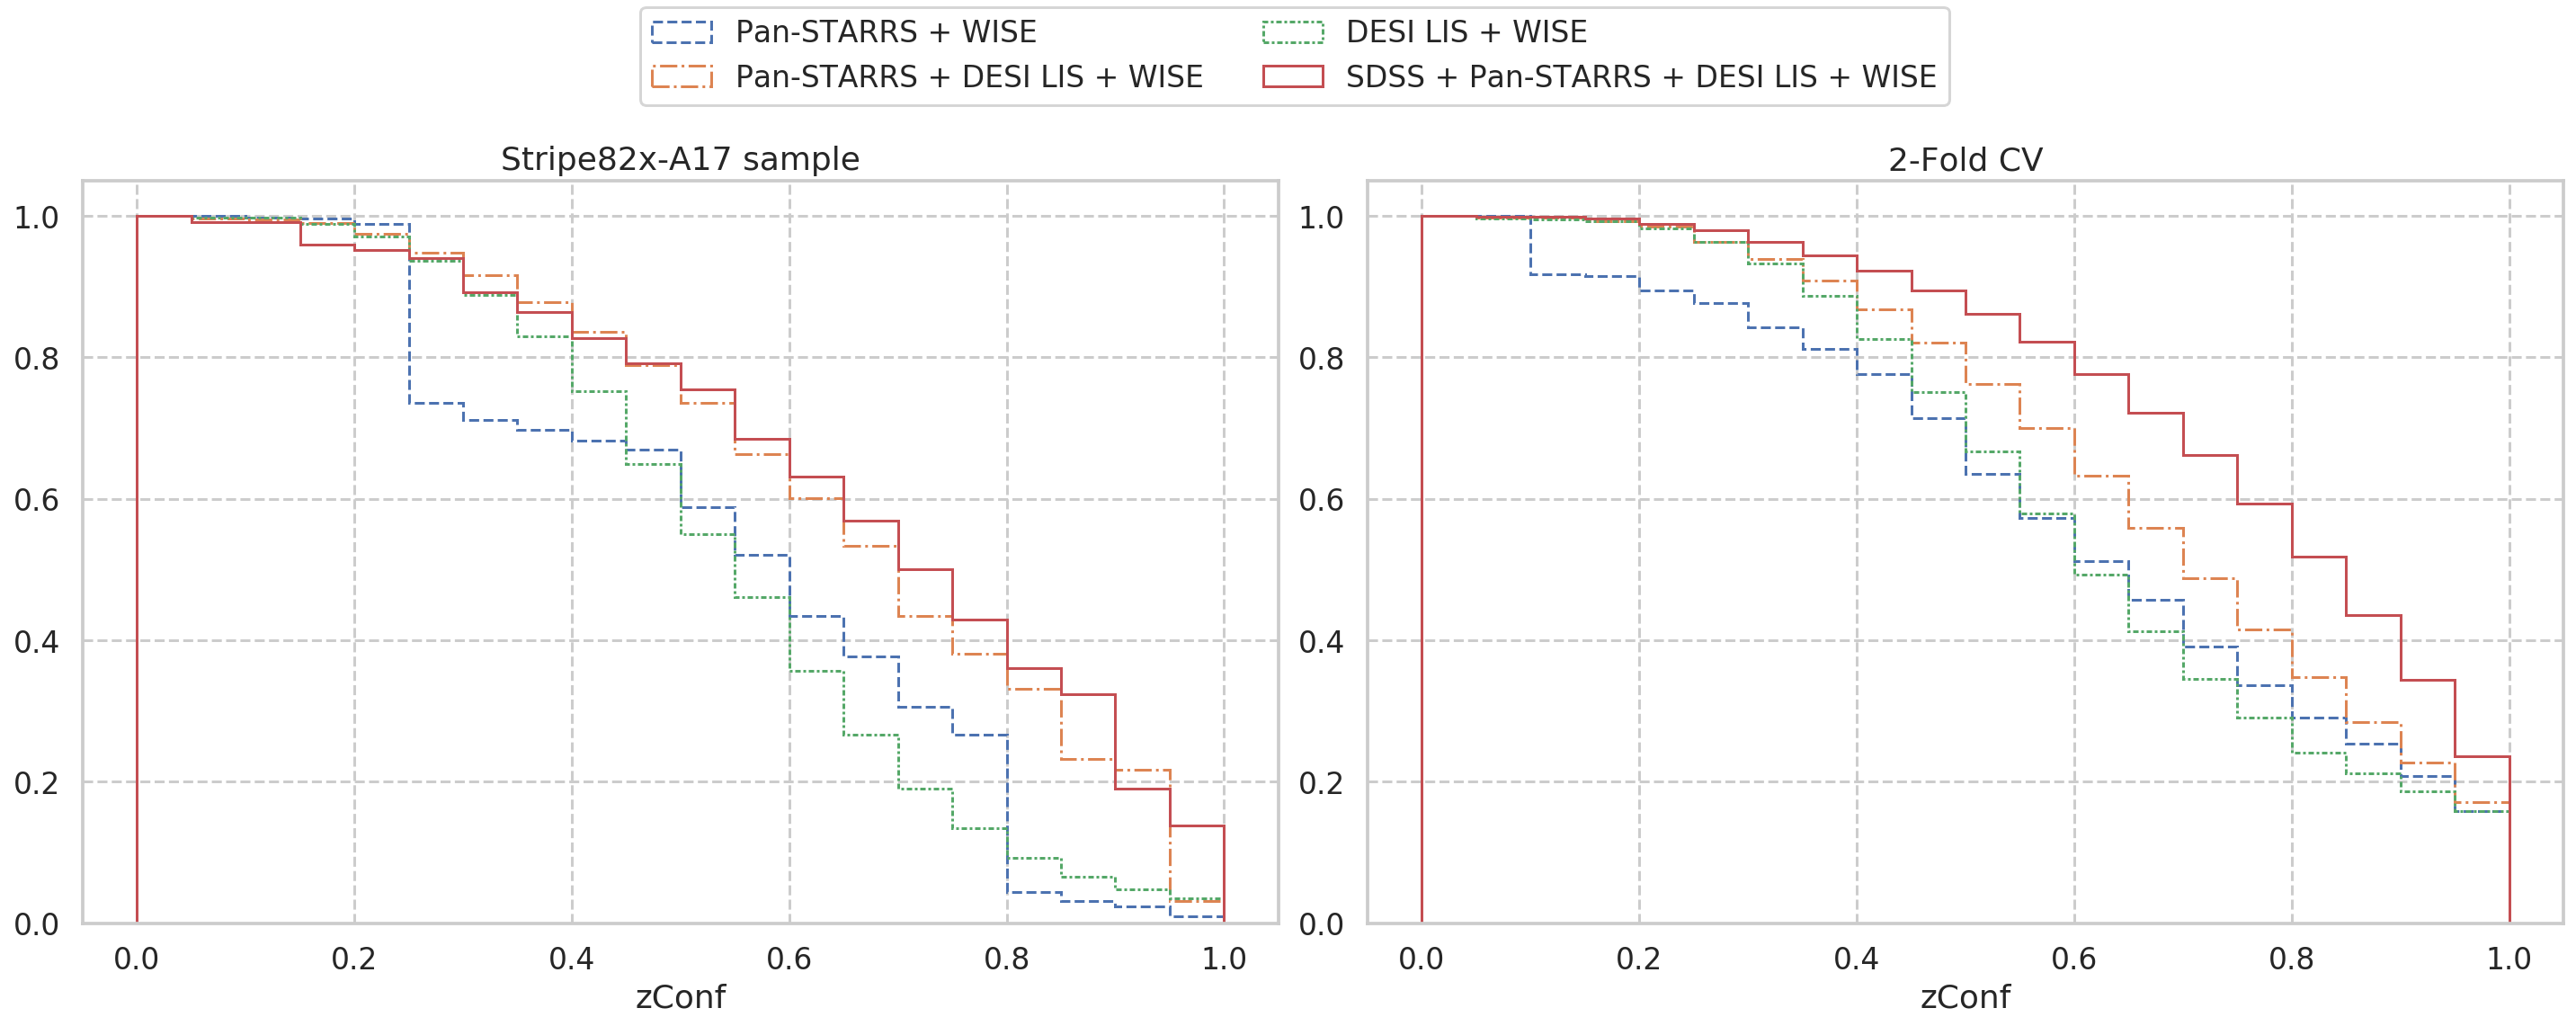
\includegraphics[width=0.9\linewidth]{images/zconf-cal.png}
    \caption{zConf distribution}
    \label{fig:zconf-cal-dr16q}
\end{figure*}

\clearpage

\subsection{Точность и полнота прогнозов}\label{ssec:precision-and-completeness}

Одной из целей работы является оценка качества моделей в контексте отбора кандидатов на далекие ($spec-z > 3$) квазары. В качестве надежных прогнозов рассматриваются прогнозы с $zConf > 0.4$. Точным будем называть прогноз, имеющий $dz_{norm}$ \eqref{eq:dznorm} меньше $0.15$.

Точность оценивалась в зависимость от величины в фильтре $z$ и от самого значения прогноза. Под этим мы имеем ввиду долю объектов с надежными прогнозами, имеющих точный прогноз (для какой доли объектов с заданным значением величины или значением прогноза и выскокой оценкой надежности zConf дан правильный прогноз), а именно \begin{equation}\label{eq:precision}
    Precision = \frac{\#\{i = \overline{1, N} | \delta z_{norm, i} < 0.15, zConf_i > 0.4\}}{\#\{i = \overline{1, N} | zConf_i > 0.4\}}.
\end{equation}

Полнота оценивалась в зависимость от величины в фильтре $z$ и от значения спектрального красного смещения. Под полнотой подразумевается доля объектов, имеющих надежный точный прогноз (какая доля объектов с заданной величиной или на заданном красном смещении будет обнаружена), а именно \begin{equation}\label{eq:completeness}
    Completeness = \frac{\#\{i = \overline{1, N} | \delta z_{norm, i} < 0.15, zConf_i > 0.4\}}{N}.
\end{equation}

На рис. \ref{fig:metrics-prec-cv2-total} приведены графики зависимости точности от значения прогноза photo-z (слева) и от оптической величины в фильтре $z$ (справа). Видно, что все модели показывают точность не ниже 0.9 на объектах $spec-z < 2.7$, кроме модели \ref{model:dw}, у которой точность падает ниже 0.85 на $spec-z \sim 1.0, 1.5, 2.5$. На оставшихся объектах точность моделей, использующих точнось только одного из каталоогов (\ref{model:dw}, \ref{model:pw}) точность может так же ухудшаться до 0.85 (на $spec-z \sim 3.3$), в то время как модели с использованием нескольких каталогов в том числе SDSS (\ref{model:spw}, \ref{model:spdw}) показывают точность выше 0.95.

Кроме того все модели имеют просадки точности на $spec-z \sim 1.0, 1.5$. Интересно, что в районе $spec-z \sim 2.1$ модель на основе признаков только DESI LIS \ref{model:dw} имеет улучшение точности, в то время как остальные модели, в том числе модель на основе признаков только Pan-STARRS \ref{model:pw}, наоборот, показывают ухудшение точности, но в итоге модель с использованием признаков и Pan-STARRS и DESI LIS \ref{model:pdw} превосходит обе "родительские" модели по точности. В этом смысле улучшение модели путем добавления других данных носит монотонный характер.

Модели с использованием данных SDSS (\ref{model:spw}, \ref{model:spdw}) показывают полноту не ниже 0.8, а на объектах $spec-z > 2.5$ -- выше 0.9, модель \ref{model:pdw} -- выше 0.7, а модели \ref{model:dw} и \ref{model:pw} на основе данныз только одного обзора -- не ниже 0.6.

Так же как $NMAD$ и доля выбросов $n_{>0.15}$, точность и полнота показывают монотонную зависимость от звездной величины в фильтре $z$. На кросс-валидации модели \ref{model:spw} и \ref{model:spdw}, использующие данные SDSS показывают полноту выше 0.7 на слабых объектах с улучшением до выше 0.9 на объектах с $z_{mag} < 20$. Модель \ref{model:pdw} -- выше 0.55 с улучшением до выше 0.8. Интересно, что модель на основе данных только DESI LIS \ref{model:dw} обеспечивает полноту на наиболее слабых объектах $\sim 0.6$, а полнота модели на основе данных только Pan-STARRS падает сильно ниже до $~0.5$. Аналогичные зависимости видны на выборке квазаров DR16q (рис. \ref{fig:metrics-prec-cv2-total}), при этом на наиболее слабых объектах увеличивается разница в полноте между моделями \ref{model:dw} и \ref{model:pw}, а модели \ref{model:pdw}, \ref{model:spw} опускаются по полноте до уровня модели \ref{model:dw}.

\begin{figure*}
    \centering
    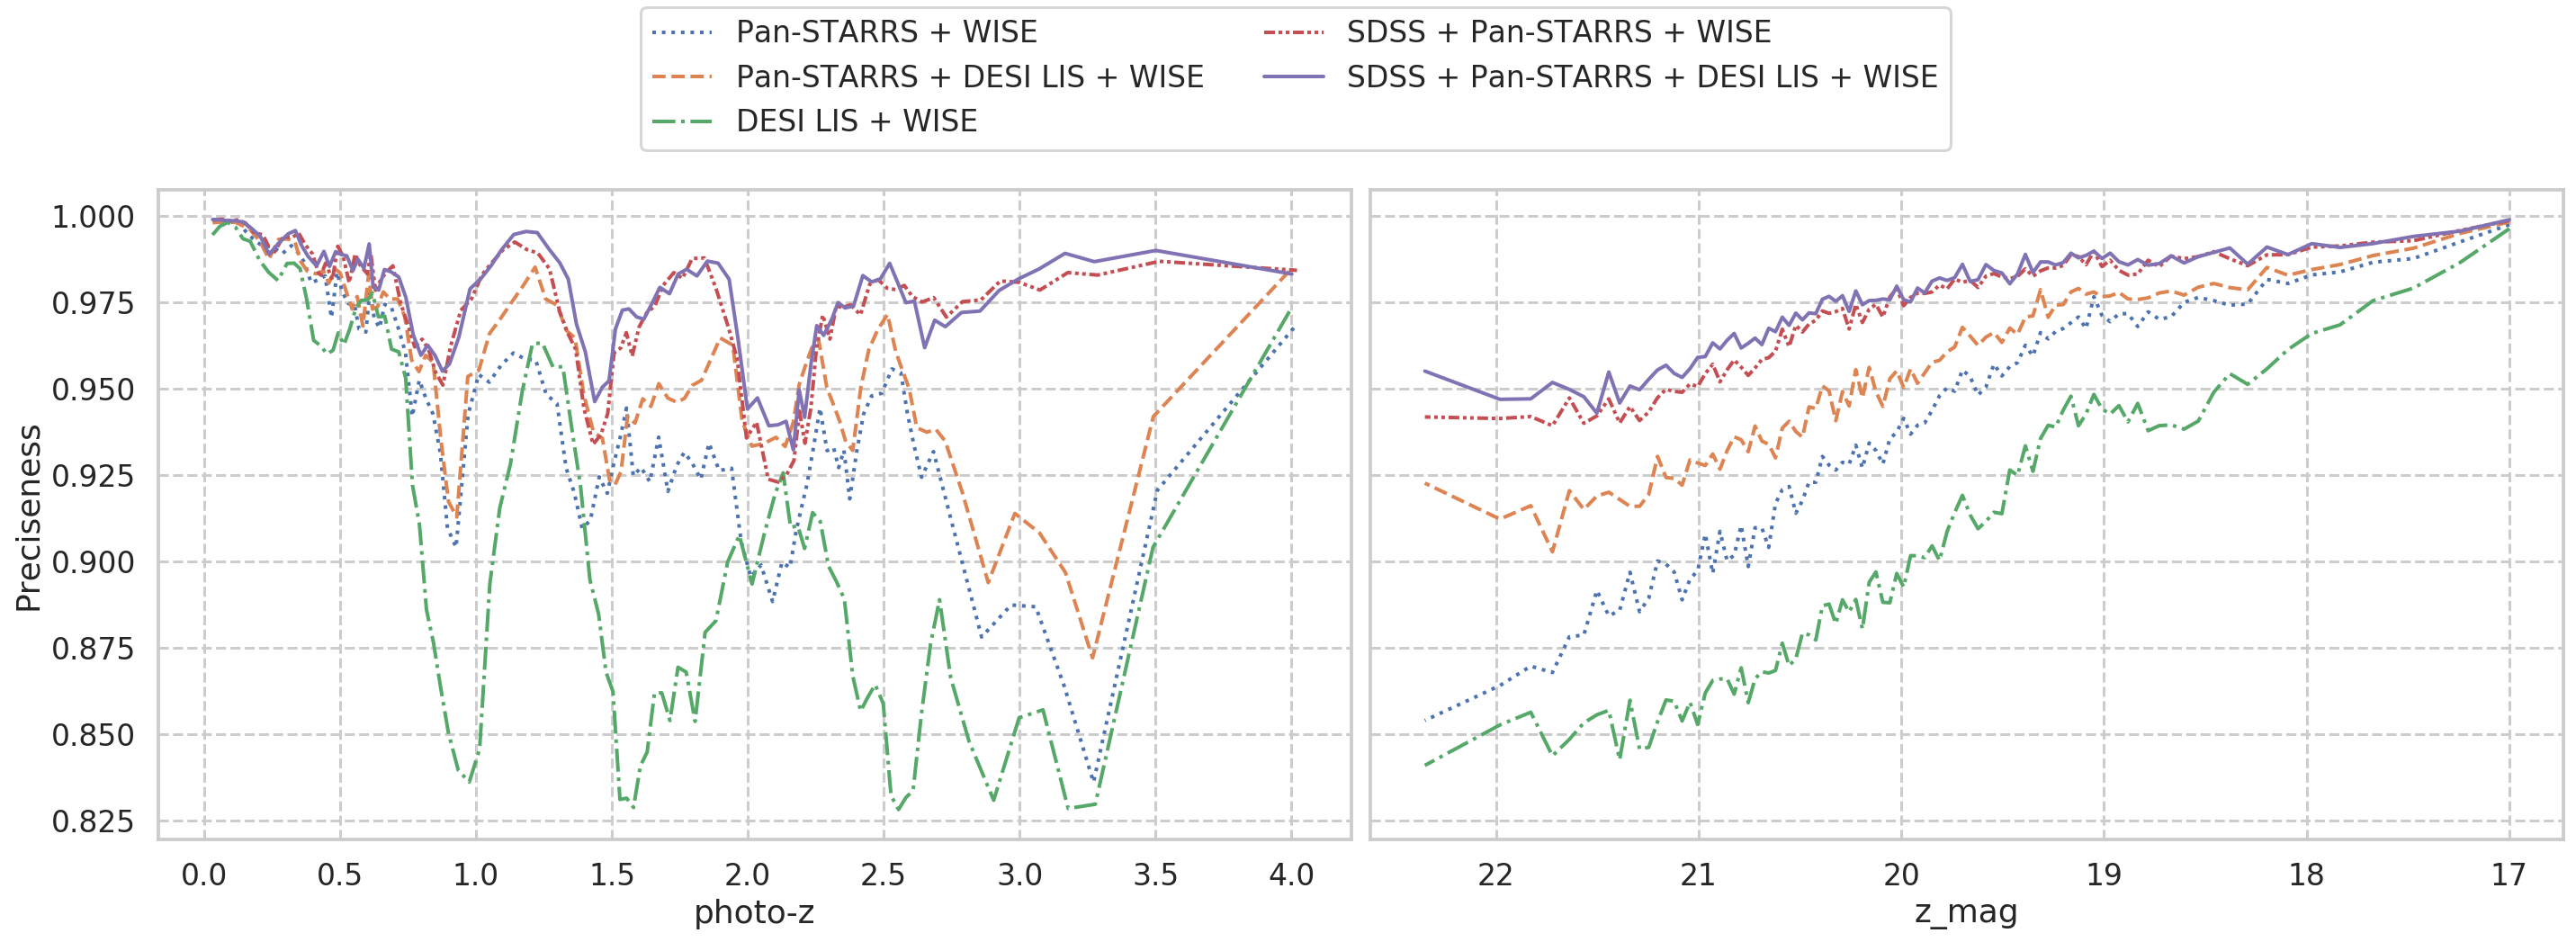
\includegraphics[width=0.9\linewidth]{images/metrics-prec-cv2.png}
    \caption{Plots of Preciseness metric as a function of (from left to right) spectral redshift value, photometric redshift prediction value, and stellar magnitude in the filter z) of cross-validation predictions. The solid line shows model \ref{model:spdw}, the dot line shows model \ref{model:pw}, the dashed line shows model \ref{model:pdw}, the dash-dot line shows model \ref{model:dw}, and dash-dot-dot line shows model \ref{model:spw}.}
    \label{fig:metrics-prec-cv2-total}
\end{figure*}

\begin{figure*}
    \centering
    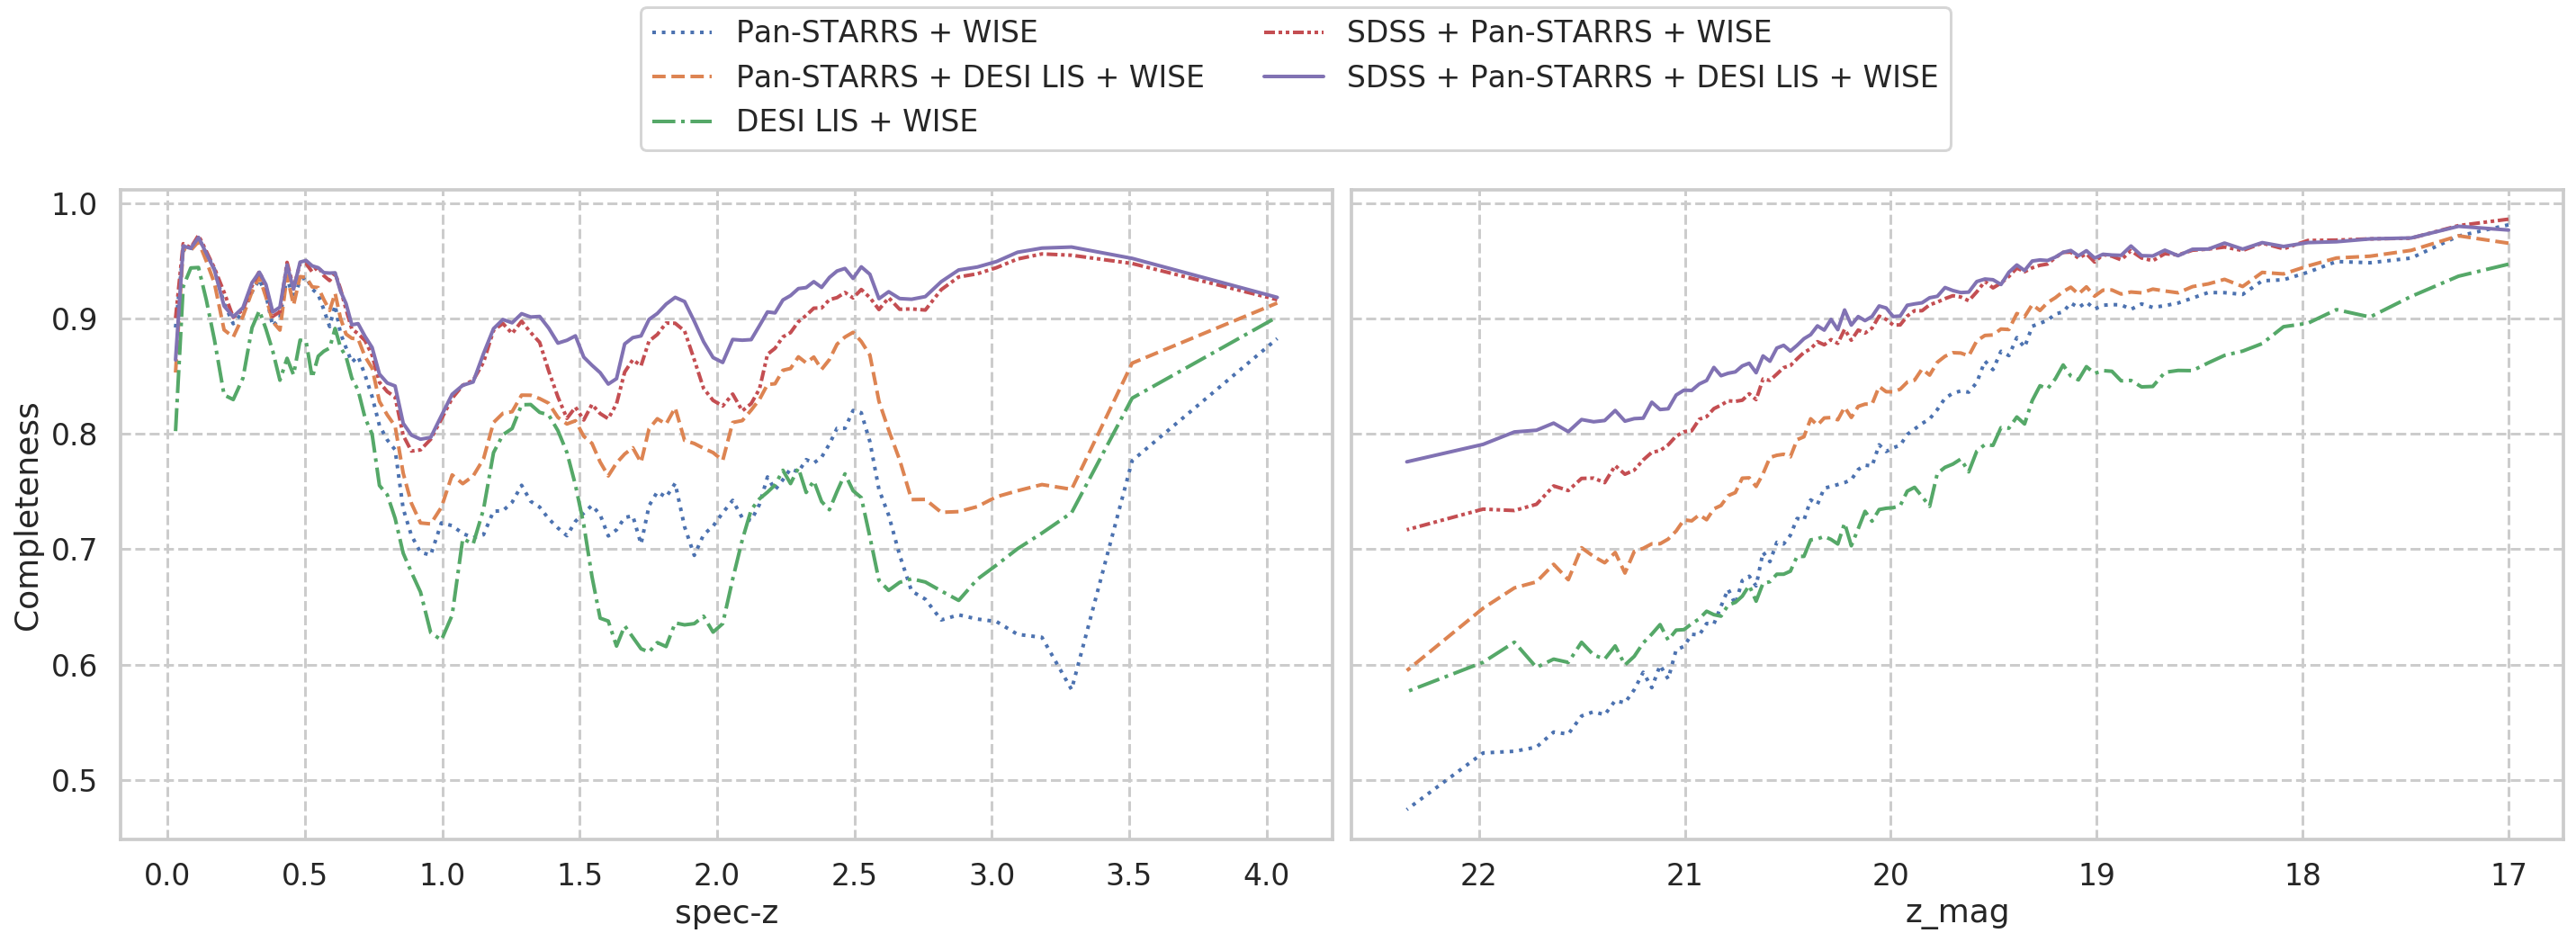
\includegraphics[width=0.9\linewidth]{images/metrics-comp-cv2.png}
    \caption{Plots of Completeness metric as a function of (from left to right) spectral redshift value, photometric redshift prediction value, and stellar magnitude in the filter z) of cross-validation predictions. The solid line shows model \ref{model:spdw}, the dot line shows model \ref{model:pw}, the dashed line shows model \ref{model:pdw}, the dash-dot line shows model \ref{model:dw}, and dash-dot-dot line shows model \ref{model:spw}.}
    \label{fig:metrics-comp-cv2-total}
\end{figure*}

\begin{figure*}
    \centering
    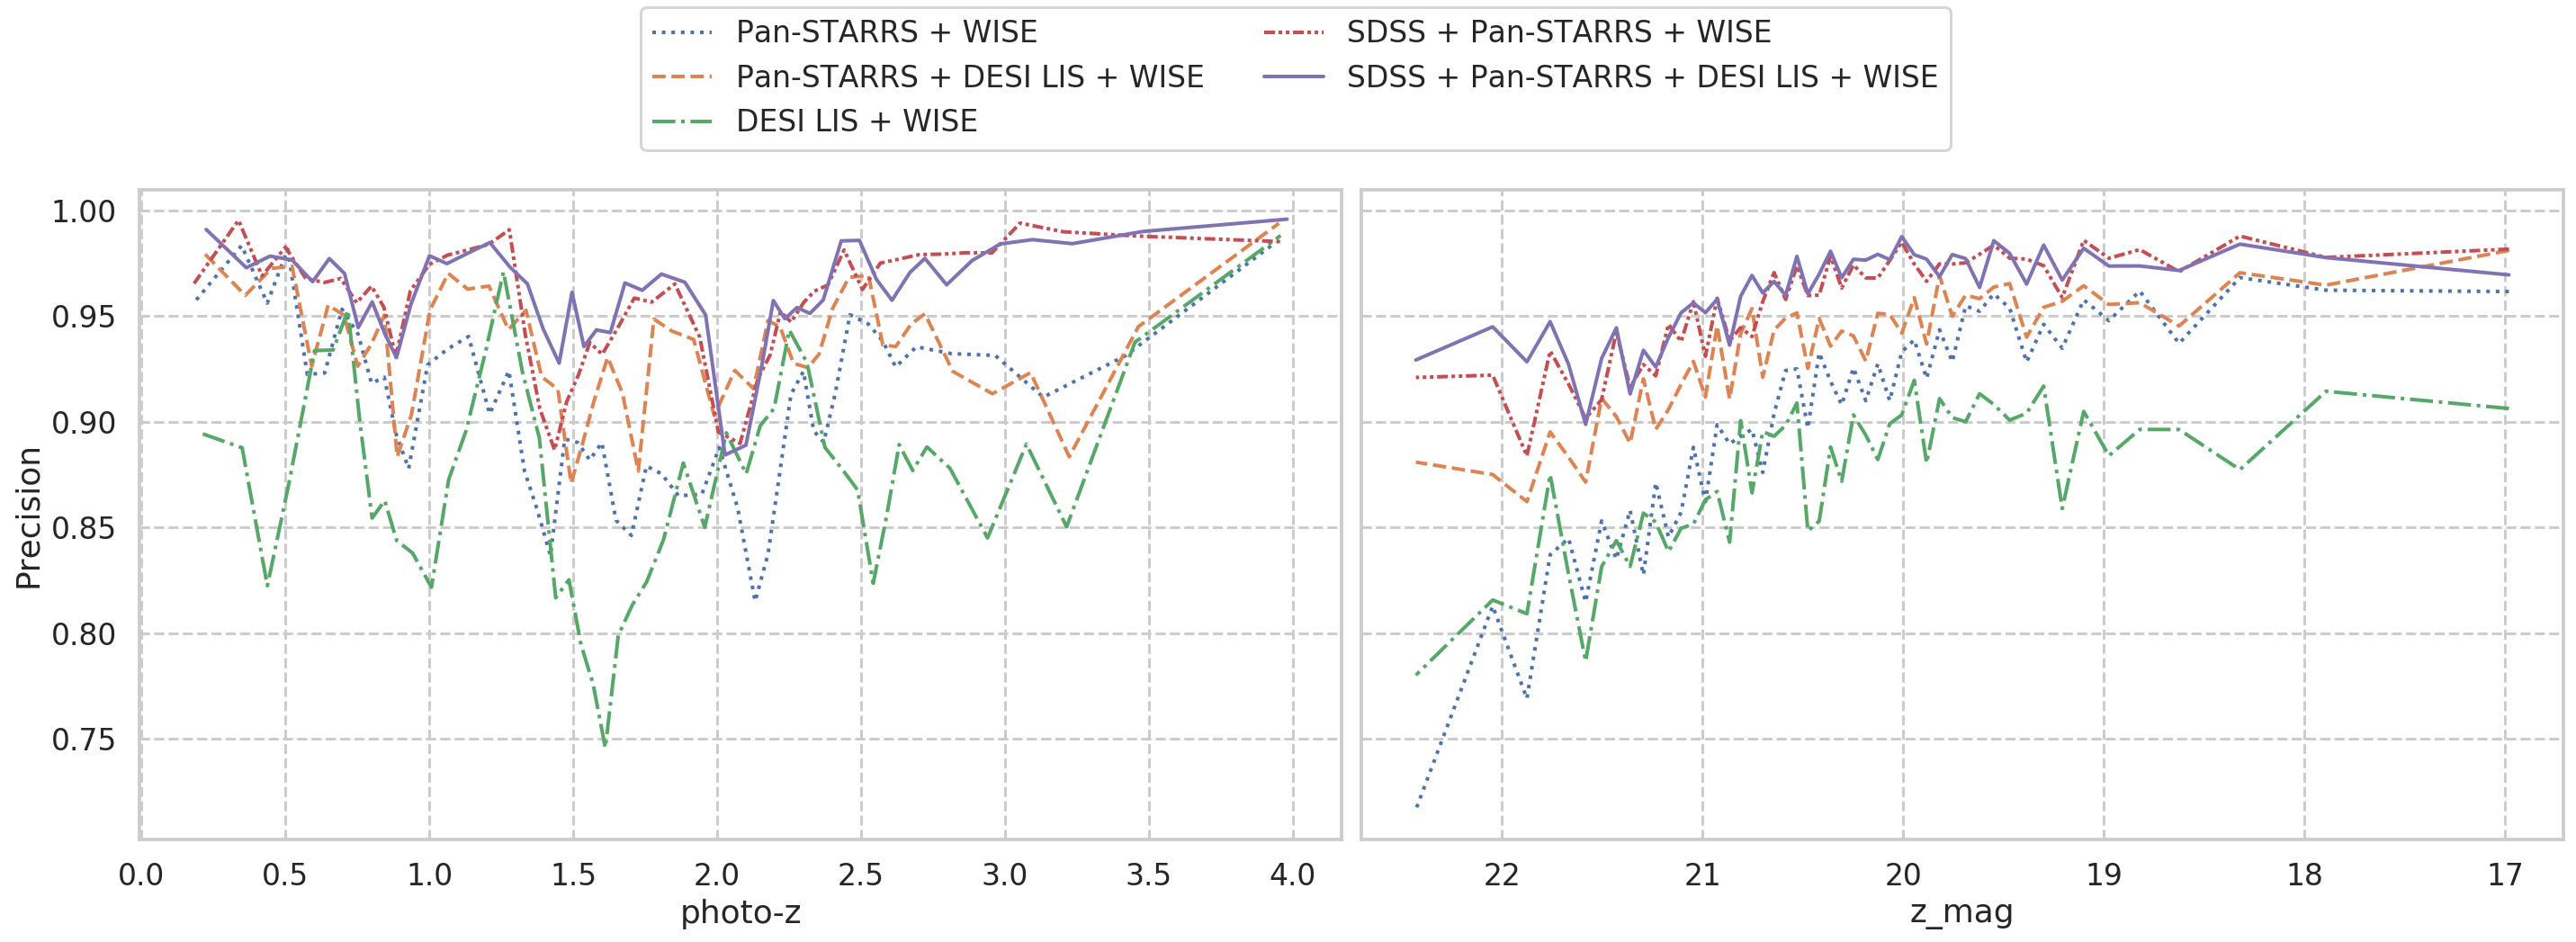
\includegraphics[width=0.9\linewidth]{images/metrics-prec-dr16q.png}
    \caption{Plots of Preciseness metric as a function of (from left to right) spectral redshift value, photometric redshift prediction value, and stellar magnitude in the filter z) on DR16q quasars test sample. The solid line shows model \ref{model:spdw}, the dot line shows model \ref{model:pw}, the dashed line shows model \ref{model:pdw}, the dash-dot line shows model \ref{model:dw}, and dash-dot-dot line shows model \ref{model:spw}.}
    \label{fig:metrics-prec-dr16q}
\end{figure*}

\begin{figure*}
    \centering
    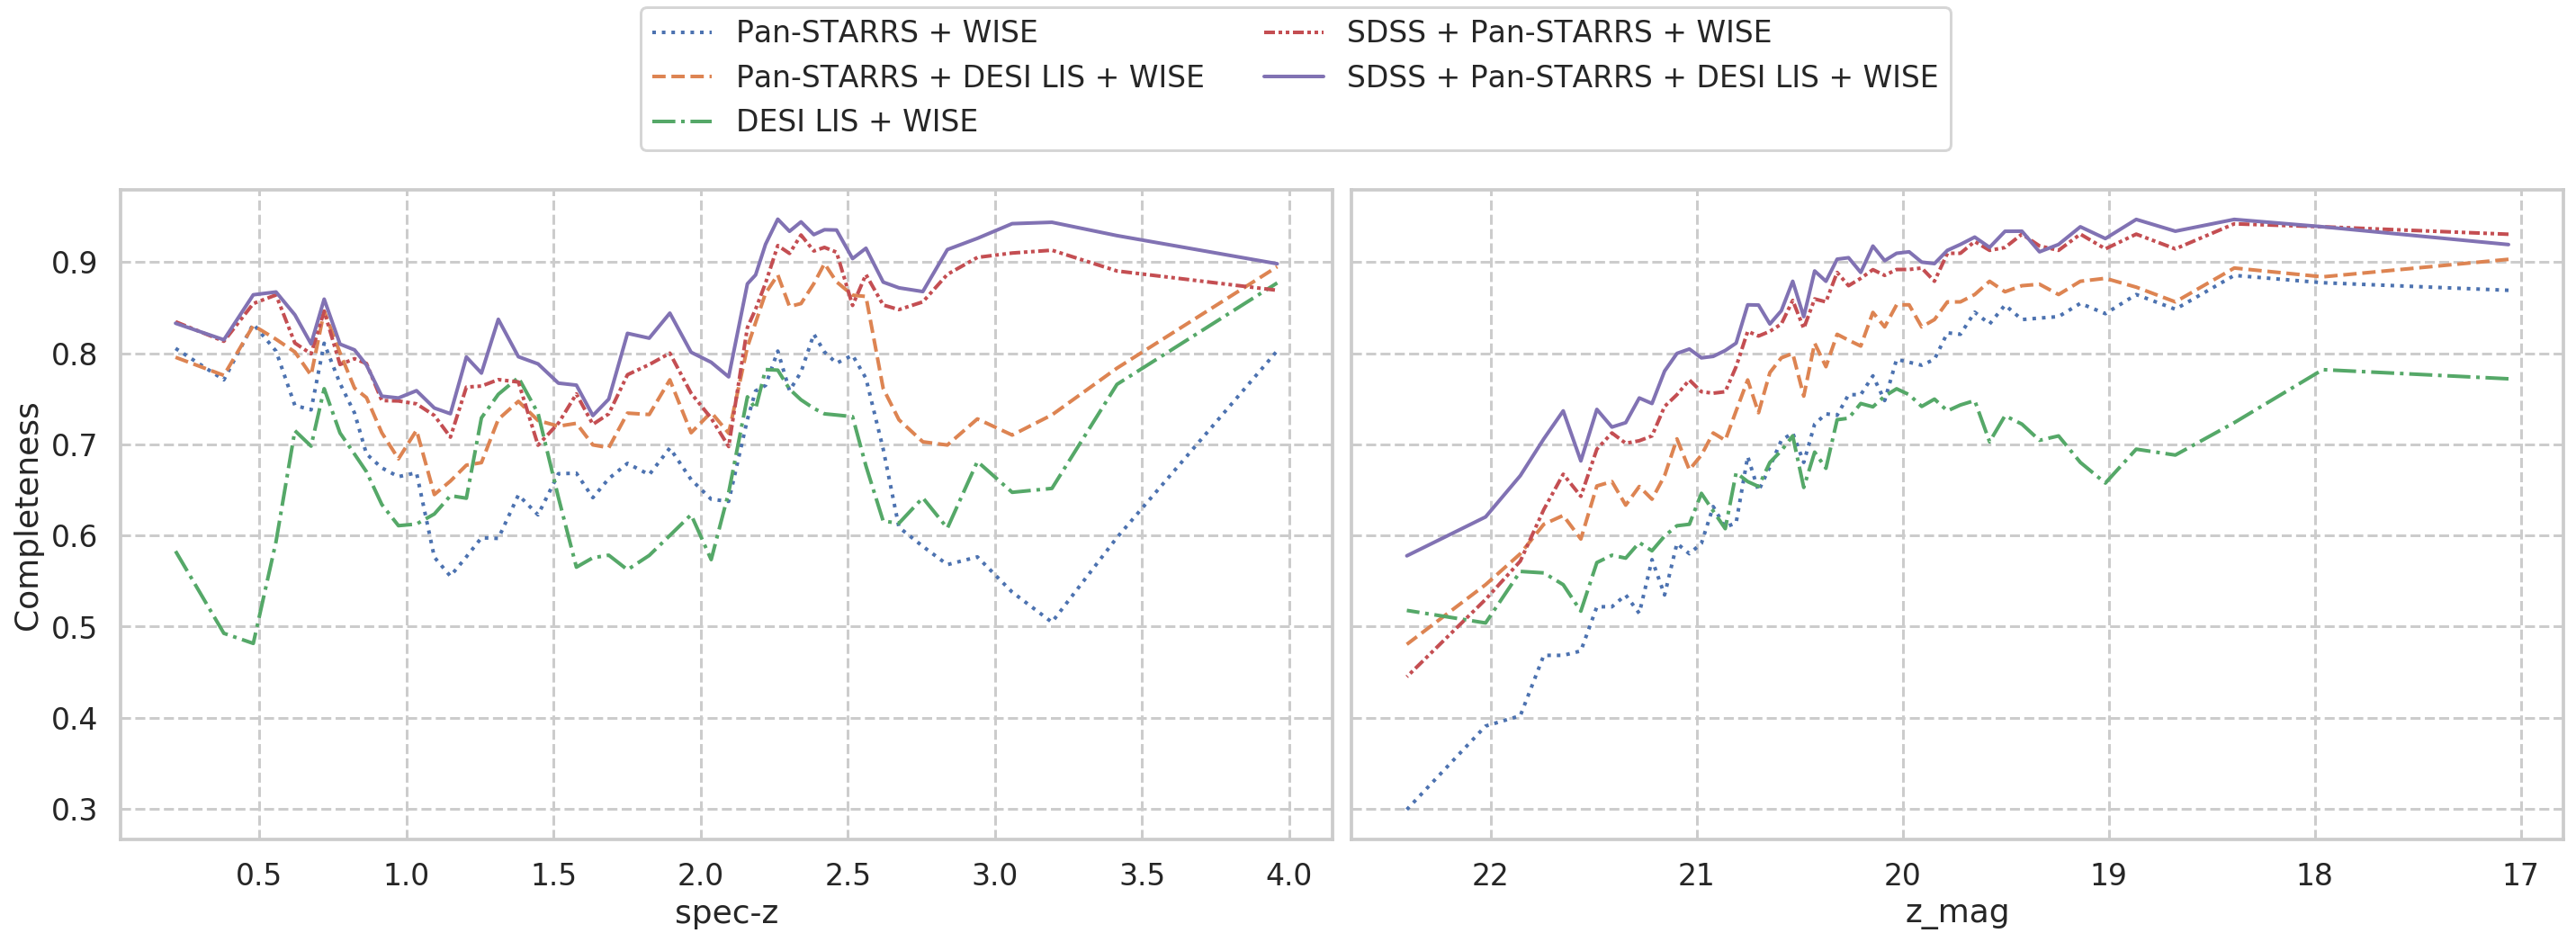
\includegraphics[width=0.9\linewidth]{images/metrics-comp-dr16q.png}
    \caption{Plots of Completeness metric as a function of (from left to right) spectral redshift value, photometric redshift prediction value, and stellar magnitude in the filter z) on DR16q quasars test sample. The solid line shows model \ref{model:spdw}, the dot line shows model \ref{model:pw}, the dashed line shows model \ref{model:pdw}, the dash-dot line shows model \ref{model:dw}, and dash-dot-dot line shows model \ref{model:spw}.}
    \label{fig:metrics-comp-dr16q}
\end{figure*}

\begin{table*}
	\begin{tabular}{lllllllllll}
            \hline
                              &                  & \multicolumn{3}{l}{Stripe82x-A17 sample} & \multicolumn{3}{l}{Quasars of DR16q} & \multicolumn{3}{l}{Cross-Validation} \\
                              &                  &               $NMAD$ &        $n>0.15$ &  $C_{68} - 0.68$ &           $NMAD$ &        $n>0.15$ &  $C_{68} - 0.68$ &           $NMAD$ &        $n>0.15$ &  $C_{68} - 0.68$ \\
            subsample & model &                      &                 &                  &                  &                 &                  &                  &                 &                  \\
            \hline
\hline
            $All$ & \ref{model:pw} &                0.056 &           0.146 &            0.028 &            0.065 &            0.17 &            0.022 &            0.047 &           0.111 &            0.045 \\
                              & \ref{model:pdw} &                0.045 &           0.107 &            0.082 &             0.05 &           0.125 &            0.062 &            0.037 &           0.085 &            0.072 \\
                              & \ref{model:dw} &                0.074 &           0.173 &  \textbf{-0.005} &            0.083 &           0.194 &  \textbf{-0.014} &            0.058 &           0.143 &  \textbf{-0.008} \\
                              & \ref{model:spw} &                0.039 &             0.1 &            0.098 &            0.041 &            0.09 &            0.077 &            0.033 &           0.055 &            0.082 \\
                              & \ref{model:spdw} &       \textbf{0.033} &  \textbf{0.084} &            0.113 &   \textbf{0.037} &  \textbf{0.078} &            0.089 &   \textbf{0.028} &  \textbf{0.048} &            0.093 \\
\hline
            $z_{spec} < 0.5$ & \ref{model:pw} &                0.035 &  \textbf{0.066} &   \textbf{0.016} &            0.038 &           0.113 &   \textbf{0.028} &            0.023 &           0.031 &   \textbf{0.003} \\
                              & \ref{model:pdw} &                 0.03 &            0.07 &            0.061 &            0.033 &           0.112 &            0.044 &            0.016 &           0.027 &            0.072 \\
                              & \ref{model:dw} &                0.048 &           0.103 &            0.042 &            0.077 &           0.197 &           -0.056 &            0.019 &           0.045 &           -0.004 \\
                              & \ref{model:spw} &                0.029 &           0.068 &            0.075 &            0.032 &  \textbf{0.085} &            0.063 &            0.021 &           0.028 &            0.022 \\
                              & \ref{model:spdw} &       \textbf{0.027} &           0.074 &            0.094 &   \textbf{0.031} &           0.097 &            0.056 &   \textbf{0.015} &  \textbf{0.025} &            0.094 \\
\hline
            $0.5 \leq z_{spec} < 1$ & \ref{model:pw} &                0.053 &           0.146 &            0.028 &            0.048 &           0.142 &             0.06 &            0.038 &           0.089 &            0.047 \\
                              & \ref{model:pdw} &                0.045 &           0.131 &            0.068 &            0.042 &           0.117 &            0.081 &             0.03 &           0.078 &             0.08 \\
                              & \ref{model:dw} &                0.081 &           0.193 &  \textbf{-0.019} &            0.086 &           0.189 &  \textbf{-0.032} &            0.049 &           0.126 &  \textbf{-0.013} \\
                              & \ref{model:spw} &                 0.04 &           0.107 &            0.109 &            0.037 &             0.1 &            0.101 &            0.031 &           0.059 &            0.089 \\
                              & \ref{model:spdw} &       \textbf{0.037} &    \textbf{0.1} &            0.122 &   \textbf{0.035} &  \textbf{0.091} &             0.12 &   \textbf{0.026} &  \textbf{0.058} &            0.111 \\
\hline
            $1 \leq z_{spec} < 1.5$ & \ref{model:pw} &                 0.08 &           0.172 &            0.025 &            0.083 &           0.194 &            0.033 &            0.069 &            0.14 &            0.056 \\
                              & \ref{model:pdw} &                0.061 &           0.108 &            0.079 &            0.068 &           0.144 &            0.069 &            0.059 &           0.099 &            0.074 \\
                              & \ref{model:dw} &                0.082 &           0.139 &   \textbf{0.012} &            0.087 &           0.176 &   \textbf{0.007} &            0.078 &           0.134 &   \textbf{0.019} \\
                              & \ref{model:spw} &                0.055 &           0.108 &            0.097 &            0.057 &           0.114 &             0.11 &            0.045 &           0.068 &            0.109 \\
                              & \ref{model:spdw} &       \textbf{0.048} &  \textbf{0.086} &            0.118 &   \textbf{0.055} &  \textbf{0.101} &            0.105 &   \textbf{0.043} &   \textbf{0.06} &            0.105 \\
\hline
            $1.5 \leq z_{spec} < 2$ & \ref{model:pw} &                0.076 &           0.154 &            0.076 &            0.077 &           0.153 &            0.088 &            0.069 &           0.136 &            0.075 \\
                              & \ref{model:pdw} &                0.044 &           0.099 &            0.127 &            0.056 &           0.125 &            0.089 &            0.051 &           0.109 &            0.077 \\
                              & \ref{model:dw} &                0.081 &           0.258 &  \textbf{-0.035} &            0.094 &           0.255 &  \textbf{-0.008} &            0.089 &           0.238 &  \textbf{-0.042} \\
                              & \ref{model:spw} &                 0.04 &           0.094 &            0.164 &            0.054 &             0.1 &            0.111 &            0.044 &           0.073 &            0.115 \\
                              & \ref{model:spdw} &       \textbf{0.031} &  \textbf{0.061} &            0.147 &   \textbf{0.045} &  \textbf{0.089} &            0.121 &   \textbf{0.038} &  \textbf{0.061} &            0.105 \\
\hline
            $2 \leq z_{spec}$ & \ref{model:pw} &                0.066 &           0.221 &  \textbf{-0.004} &            0.069 &           0.188 &           -0.028 &            0.059 &           0.142 &            0.048 \\
                              & \ref{model:pdw} &                0.043 &           0.126 &            0.096 &            0.048 &           0.122 &            0.044 &            0.047 &           0.101 &            0.064 \\
                              & \ref{model:dw} &                0.087 &           0.198 &           -0.042 &            0.078 &           0.179 &  \textbf{-0.012} &             0.08 &           0.164 &  \textbf{-0.002} \\
                              & \ref{model:spw} &                0.038 &           0.136 &            0.037 &            0.036 &           0.072 &            0.041 &            0.033 &           0.053 &            0.081 \\
                              & \ref{model:spdw} &       \textbf{0.027} &  \textbf{0.092} &            0.074 &   \textbf{0.031} &  \textbf{0.056} &            0.063 &    \textbf{0.03} &  \textbf{0.043} &            0.072 \\
\hline
            \hline
            $z_{mag} < 19$ & \ref{model:pw} &                0.035 &           0.025 &    \textbf{0.03} &            0.039 &           0.077 &            0.052 &            0.027 &           0.033 &            0.035 \\
                                   & \ref{model:pdw} &                0.026 &           0.016 &            0.069 &            0.034 &           0.069 &            0.064 &            0.019 &           0.028 &            0.077 \\
                                   & \ref{model:dw} &                0.037 &           0.064 &            0.046 &            0.071 &            0.15 &  \textbf{-0.018} &            0.026 &           0.059 &  \textbf{-0.006} \\
                                   & \ref{model:spw} &                0.023 &           0.016 &            0.098 &            0.026 &  \textbf{0.036} &            0.101 &            0.021 &           0.017 &            0.064 \\
                                   & \ref{model:spdw} &       \textbf{0.019} &  \textbf{0.009} &            0.115 &   \textbf{0.025} &           0.043 &            0.092 &   \textbf{0.017} &  \textbf{0.016} &            0.104 \\
\hline
            $19 \leq z_{mag} < 20$ & \ref{model:pw} &                0.042 &           0.077 &            0.075 &            0.046 &           0.103 &            0.059 &            0.043 &           0.079 &            0.055 \\
                                   & \ref{model:pdw} &                0.036 &           0.063 &            0.114 &            0.039 &           0.079 &            0.076 &            0.034 &           0.063 &            0.076 \\
                                   & \ref{model:dw} &                0.072 &           0.111 &  \textbf{-0.004} &            0.074 &           0.156 &  \textbf{-0.013} &            0.056 &           0.121 &  \textbf{-0.006} \\
                                   & \ref{model:spw} &                 0.03 &           0.044 &            0.116 &            0.031 &            0.05 &            0.094 &             0.03 &           0.037 &            0.088 \\
                                   & \ref{model:spdw} &       \textbf{0.029} &   \textbf{0.04} &            0.131 &   \textbf{0.029} &  \textbf{0.044} &            0.099 &   \textbf{0.026} &  \textbf{0.034} &            0.097 \\
\hline
            $20 \leq z_{mag} < 20.5$ & \ref{model:pw} &                0.063 &            0.13 &            0.036 &            0.062 &           0.153 &            0.016 &            0.059 &            0.13 &            0.055 \\
                                   & \ref{model:pdw} &                0.046 &           0.109 &            0.099 &            0.046 &           0.114 &            0.062 &            0.047 &           0.098 &            0.072 \\
                                   & \ref{model:dw} &                0.078 &           0.173 &   \textbf{0.001} &            0.079 &           0.181 &  \textbf{-0.008} &             0.08 &           0.171 &  \textbf{-0.008} \\
                                   & \ref{model:spw} &                0.041 &           0.081 &             0.11 &            0.038 &           0.067 &            0.075 &            0.037 &           0.058 &            0.097 \\
                                   & \ref{model:spdw} &       \textbf{0.033} &   \textbf{0.07} &             0.11 &   \textbf{0.033} &  \textbf{0.058} &            0.094 &   \textbf{0.034} &  \textbf{0.053} &            0.096 \\
\hline
            $20.5 \leq z_{mag} < 21$ & \ref{model:pw} &                0.079 &           0.201 &           -0.007 &            0.075 &           0.188 &            0.014 &            0.071 &           0.169 &            0.044 \\
                                   & \ref{model:pdw} &                0.055 &           0.117 &             0.08 &            0.054 &           0.131 &            0.074 &            0.056 &           0.126 &            0.064 \\
                                   & \ref{model:dw} &                0.087 &           0.207 &   \textbf{0.004} &            0.084 &           0.199 &  \textbf{-0.006} &            0.089 &           0.204 &   \textbf{-0.01} \\
                                   & \ref{model:spw} &                0.054 &           0.126 &            0.083 &            0.047 &           0.099 &            0.059 &            0.045 &           0.083 &            0.084 \\
                                   & \ref{model:spdw} &       \textbf{0.041} &  \textbf{0.101} &            0.109 &    \textbf{0.04} &  \textbf{0.083} &            0.085 &    \textbf{0.04} &  \textbf{0.071} &            0.083 \\
\hline
            $21 \leq z_{mag} < 23$ & \ref{model:pw} &                0.123 &           0.318 &  \textbf{-0.011} &            0.107 &           0.266 &  \textbf{-0.015} &            0.089 &           0.213 &             0.04 \\
                                   & \ref{model:pdw} &                0.079 &           0.234 &            0.043 &            0.073 &           0.185 &            0.043 &            0.066 &           0.156 &            0.065 \\
                                   & \ref{model:dw} &                0.114 &           0.315 &           -0.063 &            0.099 &           0.245 &           -0.022 &            0.096 &           0.229 &  \textbf{-0.011} \\
                                   & \ref{model:spw} &                0.082 &            0.25 &            0.081 &            0.066 &           0.155 &            0.065 &            0.054 &           0.111 &            0.084 \\
                                   & \ref{model:spdw} &       \textbf{0.063} &  \textbf{0.204} &            0.095 &   \textbf{0.055} &  \textbf{0.127} &             0.08 &   \textbf{0.048} &  \textbf{0.093} &             0.08 \\
\hline
            \hline
            \end{tabular}
            \caption{Prediction metrics for models \ref{model:pw} -- \ref{model:spdw}. The first column shows the subsample of the whole sample, the second column the model number. The next three columns -- NMAD \eqref{eq:nmad}, catastrophic outliers fraction \eqref{eq:n015}, and 68\% confidence interval calibration \eqref{eq:c68} metrics on the Stripe82X X-ray object test sample, the second three columns -- on the SDSS DR16q quasar test sample, and the last three columns -- on cross-validation.}
            \label{tab:total_metrics_table}
\end{table*}



\begin{table*}
	\begin{tabular}{lllllrllllrllllr}
            \hline
            {} & \multicolumn{5}{l}{$FSoft \geq 3e-15$ (2653 objects)} & \multicolumn{5}{l}{$FSoft \geq 1e-14$ (1501 objects)} & \multicolumn{5}{l}{$FSoft \geq 4e-14$ (242 objects)} \\
            {} &                         Precision &     $C_{preds}$ &   $C_{secureO}$ &     $C_{Xray}$ & $N_{preds}$ &                         Precision &     $C_{preds}$ &   $C_{secureO}$ &      $C_{Xray}$ & $N_{preds}$ &                        Precision &     $C_{preds}$ &   $C_{secureO}$ &      $C_{Xray}$ & $N_{preds}$ \\
            Model &                                   &                 &                 &                &             &                                   &                 &                 &                 &             &                                  &                 &                 &                 &             \\
            \hline
            PW    &                             0.935 &           0.726 &           0.597 &          0.304 &        2183 &                             0.937 &           0.773 &           0.659 &           0.427 &        1280 &                            0.944 &           0.876 &            0.76 &           0.546 &         210 \\
            PDW   &                             0.944 &           0.762 &           0.637 &          0.325 &        2220 &                             0.948 &           0.807 &           0.692 &           0.449 &        1287 &                            0.953 &           0.876 &            0.76 &           0.546 &         210 \\
            DW    &                             0.885 &            0.67 &  \textbf{0.666} &  \textbf{0.34} &        2639 &                              0.89 &           0.704 &           0.701 &           0.455 &        1494 &                            0.882 &            0.72 &           0.711 &            0.51 &         239 \\
            SPW   &                             0.963 &           0.794 &           0.647 &           0.33 &        2162 &                              0.97 &           0.846 &           0.716 &           0.464 &        1270 &                            0.964 &           0.904 &           0.777 &           0.558 &         208 \\
            SPDW  &                    \textbf{0.969} &  \textbf{0.805} &  \textbf{0.666} &  \textbf{0.34} &        2197 &                    \textbf{0.975} &  \textbf{0.849} &  \textbf{0.722} &  \textbf{0.468} &        1276 &                   \textbf{0.974} &  \textbf{0.918} &  \textbf{0.789} &  \textbf{0.567} &         208 \\
            \hline
            \end{tabular}
            \caption{Prediction metrics for models \ref{model:pw} -- \ref{model:spdw} from Stripe82X X-ray test sample. The first column shows model, the next two columns -- Precision \ref{eq:precision} and Completeness \ref{eq:completeness} metrics for objects with $FSoft < 1e-14$, the second two columns -- for objects with $FSoft < 4e-14$, and the last two columns -- for the entire sample.}
\end{table*}

% \begin{table*}
% 	\begin{tabular}{lllllll}
%             \hline
%             {} & \multicolumn{2}{l}{$FSoft \geq 3e-15$ (2170 objects)} & \multicolumn{2}{l}{$FSoft \geq 1e-14$ (1272 objects)} & \multicolumn{2}{l}{$FSoft \geq 4e-14$ (207 objects)} \\
%             {} &                         Precision &    Completeness &                         Precision &    Completeness &                        Precision &    Completeness \\
%             Model &                                   &                 &                                   &                 &                                  &                 \\
%             \hline
%             PW    &                             0.936 &           0.724 &                             0.939 &           0.774 &                            0.948 &           0.879 \\
%             PDW   &                             0.945 &           0.763 &                             0.948 &           0.807 &                            0.958 &           0.879 \\
%             DW    &                             0.883 &           0.674 &                             0.884 &           0.704 &                            0.877 &           0.725 \\
%             SPW   &                             0.963 &           0.789 &                              0.97 &           0.843 &                            0.964 &           0.903 \\
%             SPDW  &                    \textbf{0.968} &  \textbf{0.805} &                    \textbf{0.975} &  \textbf{0.847} &                   \textbf{0.974} &  \textbf{0.918} \\
%             \hline
%             \end{tabular}
%             \caption{Prediction metrics for models \ref{model:pw} -- \ref{model:spdw} from Stripe82X X-ray test sample. The first column shows model, the next two columns -- Precision \ref{eq:precision} and Completeness \ref{eq:completeness} metrics for objects with $FSoft < 1e-14$, the second two columns -- for objects with $FSoft < 4e-14$, and the last two columns -- for the entire sample.}
% \end{table*}

% ===============================================================================
% ===============================================================================
% ===============================================================================

\section{Conclusion and discussion}\label{sec:conclusion}

% В рамках работы было построено множество моделей photo-z на основе различных признаков, которые строятся по данным трех современных фотометрических обзоров~--- SDSS, Pan-STARRS1 и DESI Legacy Imaging Survey. Обучающая выборка состоит из $\sim$580000 оптических квазаров и галактик и сбалансирована, чтобы аппроксимировать распределение рентгеновских объектов. Разметка взята из спектрального каталога оптических объектов SDSS.

% На тестовой выборке рентгеновских объектов поля Stripe82X \cite{bib:ananna}, за счет использования данных всех трех вышеупомянутых обзоров, была достигнута точность по метрикам $NMAD$ и доля выбросов $n_{>0.15}$ значительно выше (почти в 2 раза), чем точность лучших моделей известных в литературе (SOTA), что является основным результатом работы. Для лучшей модели / шаблонной модели \cite{bib:ananna} / нейросетевой модели \cite{bib:brescia} на выборке Stripe82X получены значения метрик $NMAD$ = 0.034 / 0.065 / 0.066 и $n_{>0.15}$ = 0.088 / 0.170 / 0.156, соответственно.

The proposed photo-z models based on Random Forests show accuracy (up to 2 times) better than current SOTA results in the literature (on Stripe82X field). The main accuracy improvement comes from using a large training sample ($\sim$600k objects) with features from modern wide photometric surveys. First optical spectroscopic observations of eRosita sources show that the proposed photo-z models are effective in the ongoing search for distant X-ray quasars (see e.g. \citep{2020MNRAS.497.1842M,2020AstL...46..149K,2020AstL...46..429D}).

The presented photo-z models are integrated into the SRGz system designed to construct a three-dimensional map of X-ray sources on the Eastern Galactic Hemisphere of the SRG/eRosita All-Sky survey. The SRGz system is developed in the science working group of RU eROSITA consortium on X-ray source detection, identification, and eROSITA source catalog in the High Energy Astrophysics Department at Space Research Institute of the Russian Academy of Sciences.

% ===============================================================================
% ===============================================================================
% ===============================================================================

Провалы в точности по zspec. Переход на ансамбли нейронных сетей. Источник данных о поглощении на всем небе?

\clearpage

\section*{Acknowledgments}
..

% bibliograpgy 
\bibliographystyle{mnras}
\bibliography{main}

\appendix

%\section{Advanced metrics charts}
%
%\begin{landscape}
%\begin{figure}
%    \centering
%    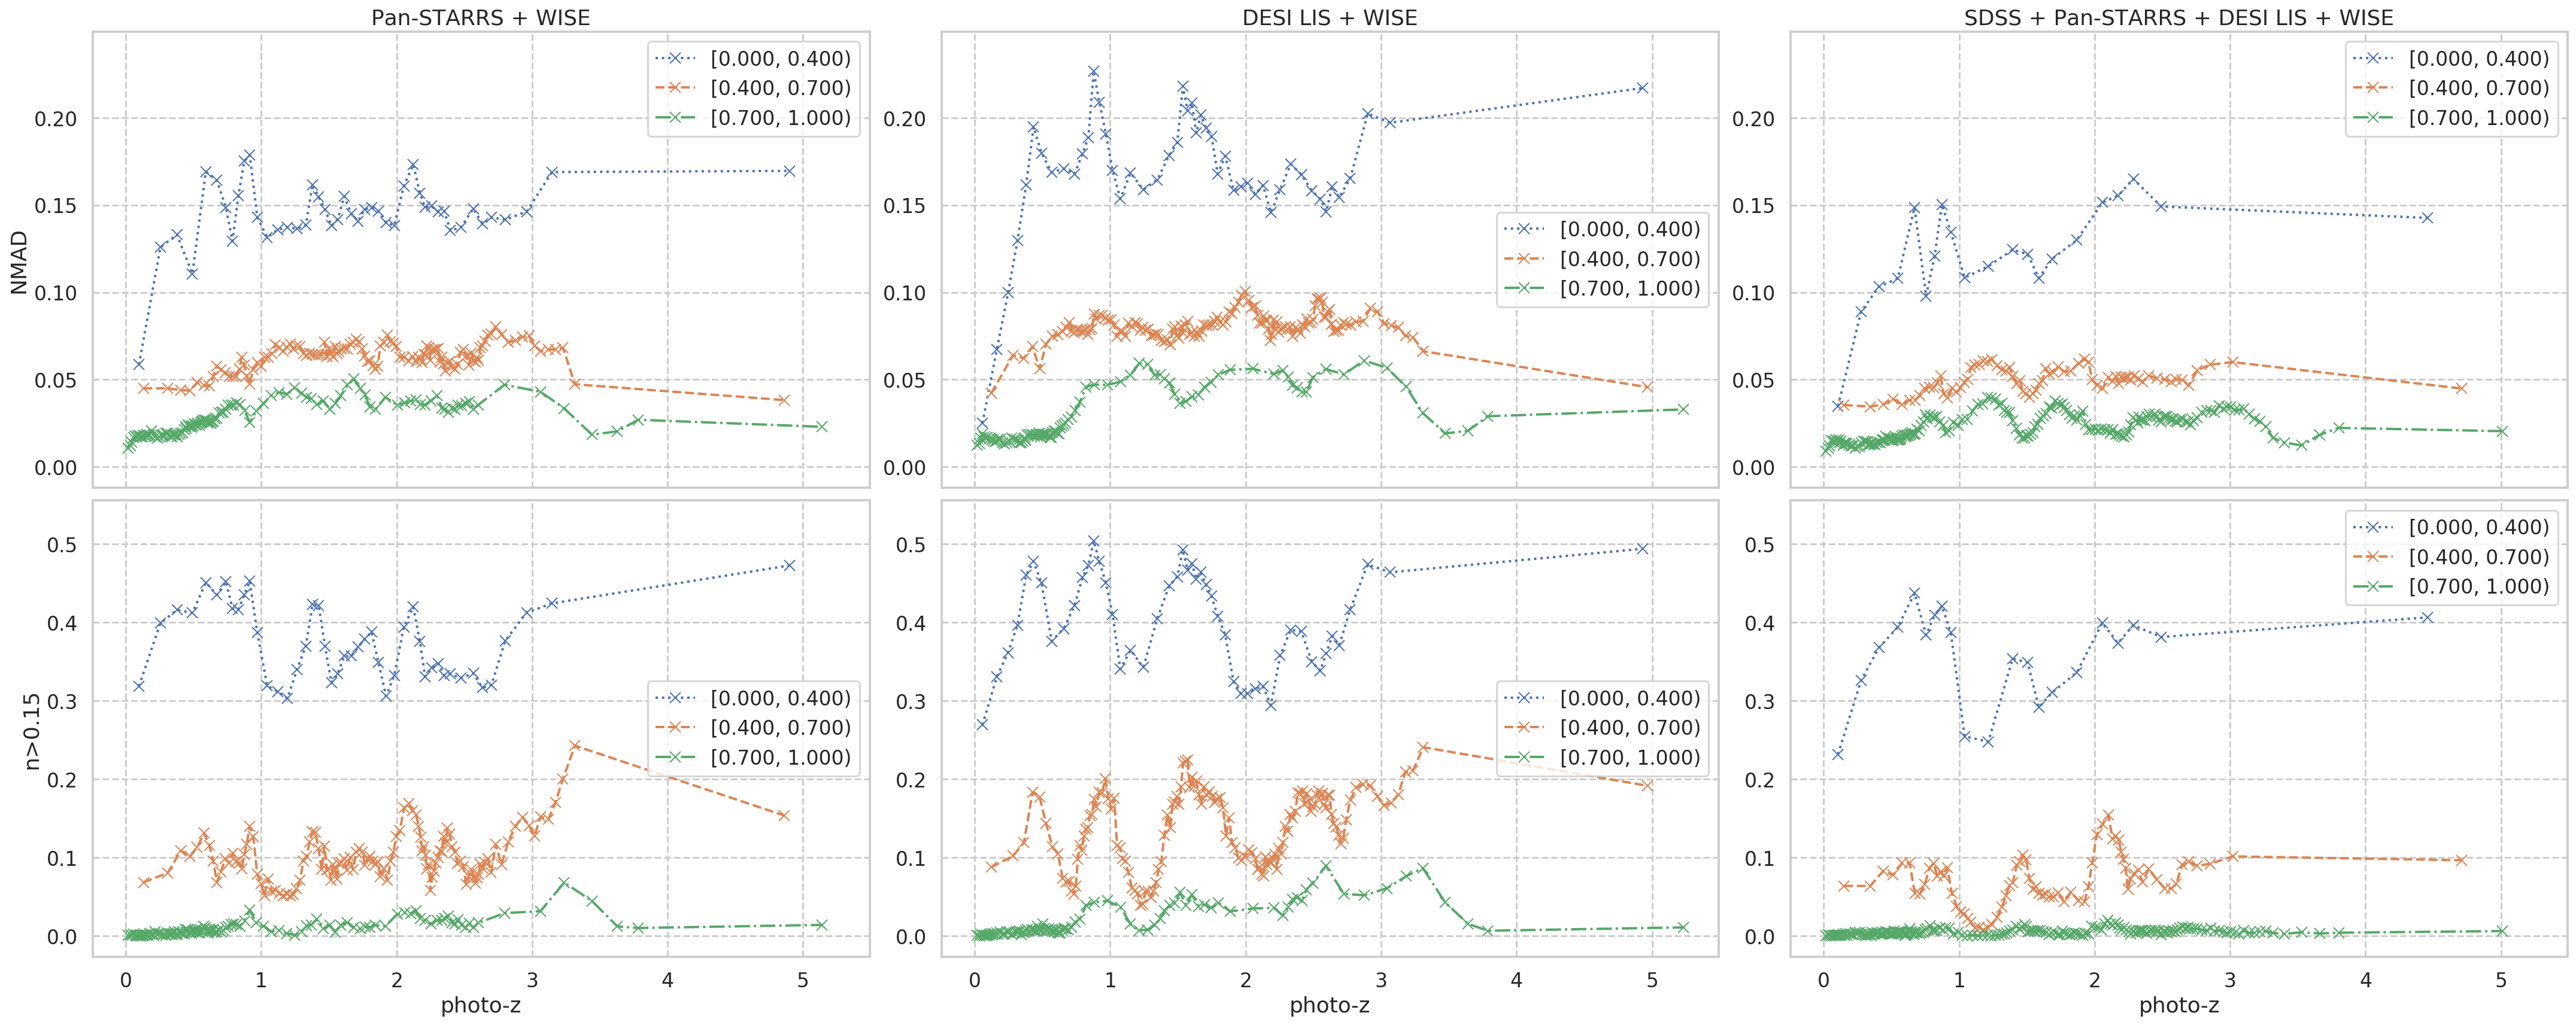
\includegraphics[width=25cm]{images/metrics-adv-photoz-x-zconf-cv2.png}
%    \caption{Метрики в зависимости от photo-z для разных порогов по zConf на кросс-валидации}
%    \label{fig:my_label}
%\end{figure}
%\end{landscape}
%
%
%\begin{landscape}
%\begin{figure}
%    \centering
%    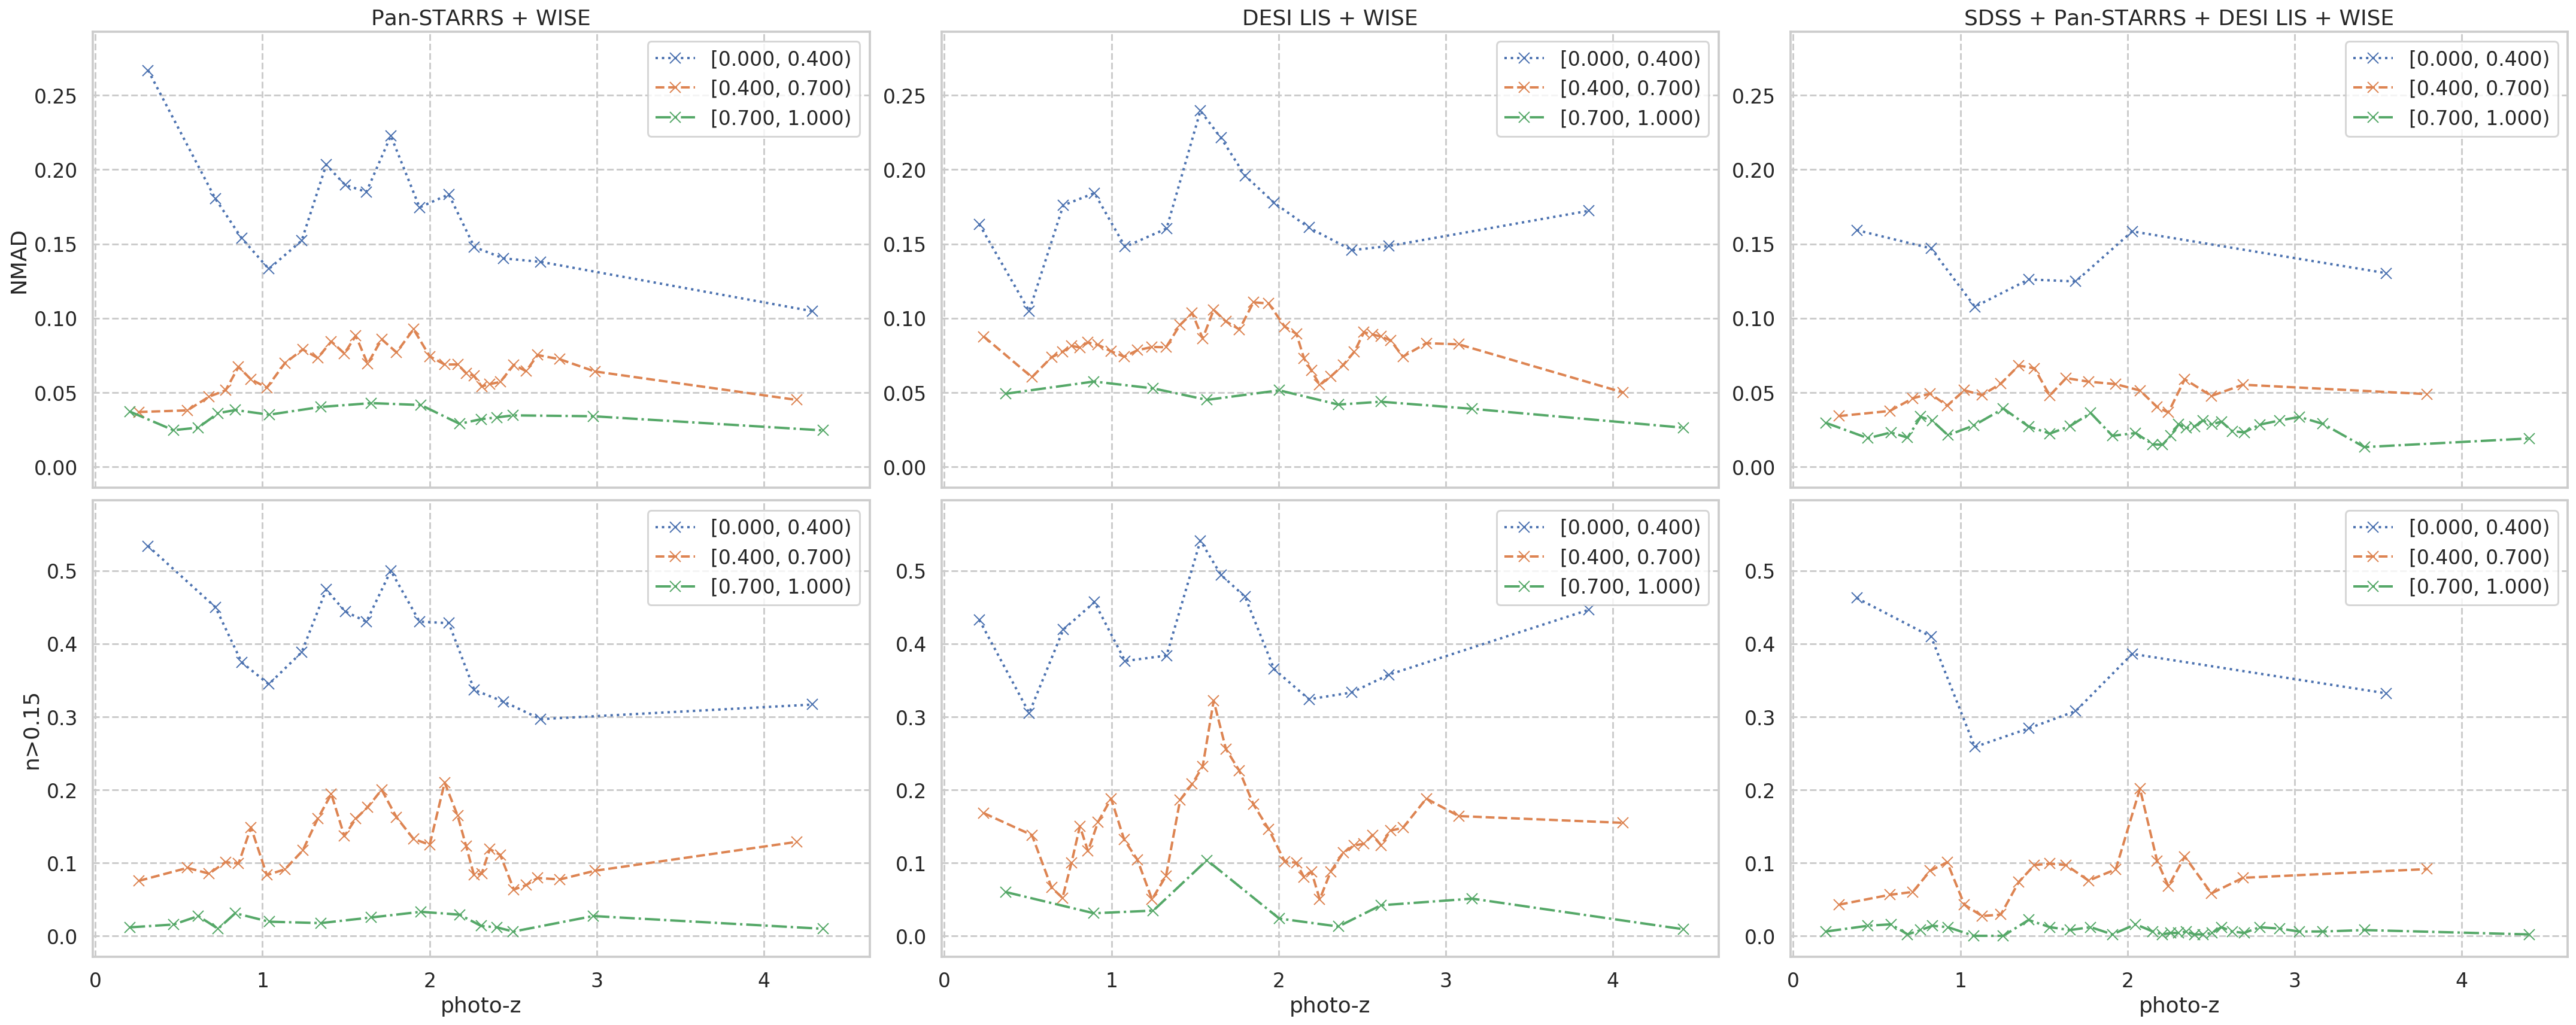
\includegraphics[width=0.9\linewidth]{images/metrics-adv-photoz-x-zconf-dr16q.png}
%    \caption{Метрики в зависимости от photo-z для разных порогов по zConf на DR16q}
%    \label{fig:my_label}
%\end{figure}
%\end{landscape}
%
%
%\begin{landscape}
%\begin{figure}
%    \centering
%    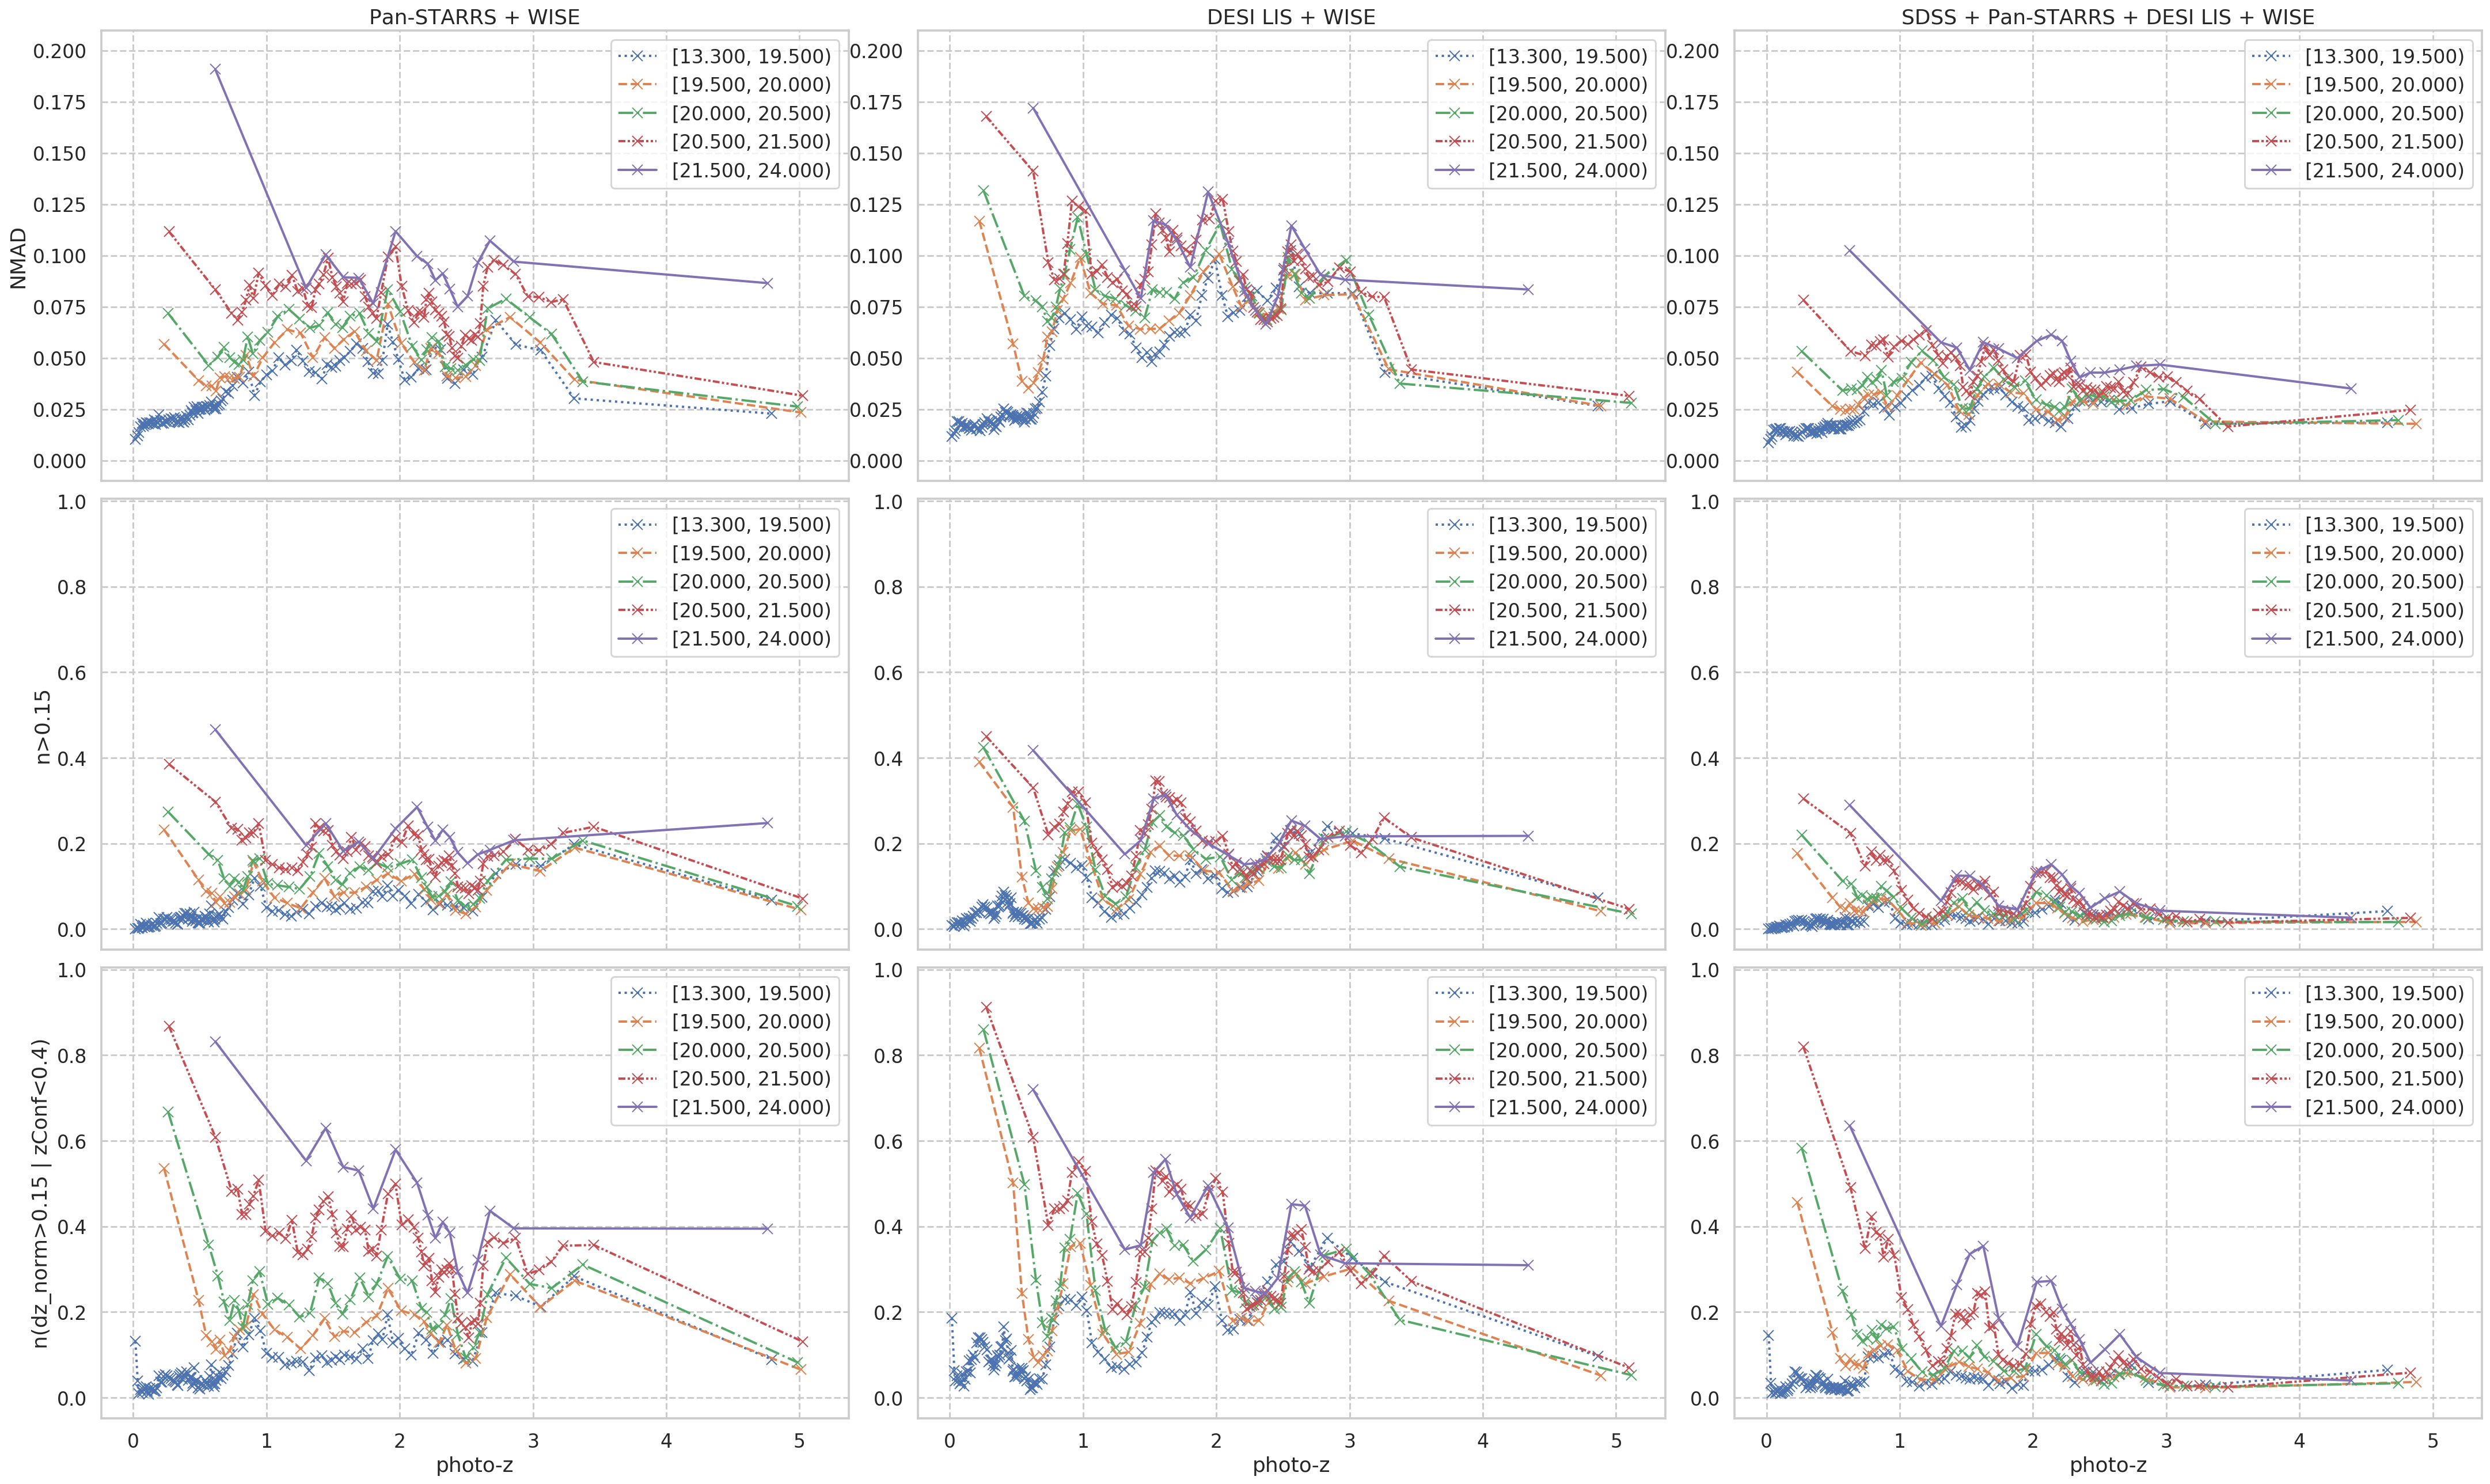
\includegraphics[width=0.9\linewidth]{images/metrics-adv-photoz-x-zmag-cv2.png}
%    \caption{Метрики в зависимости от photo-z для разных порогов по $z_mag$ на кросс-валидации}
%    \label{fig:my_label}
%\end{figure}
%\end{landscape}
%
%
%\begin{landscape}
%\begin{figure}
%    \centering
%    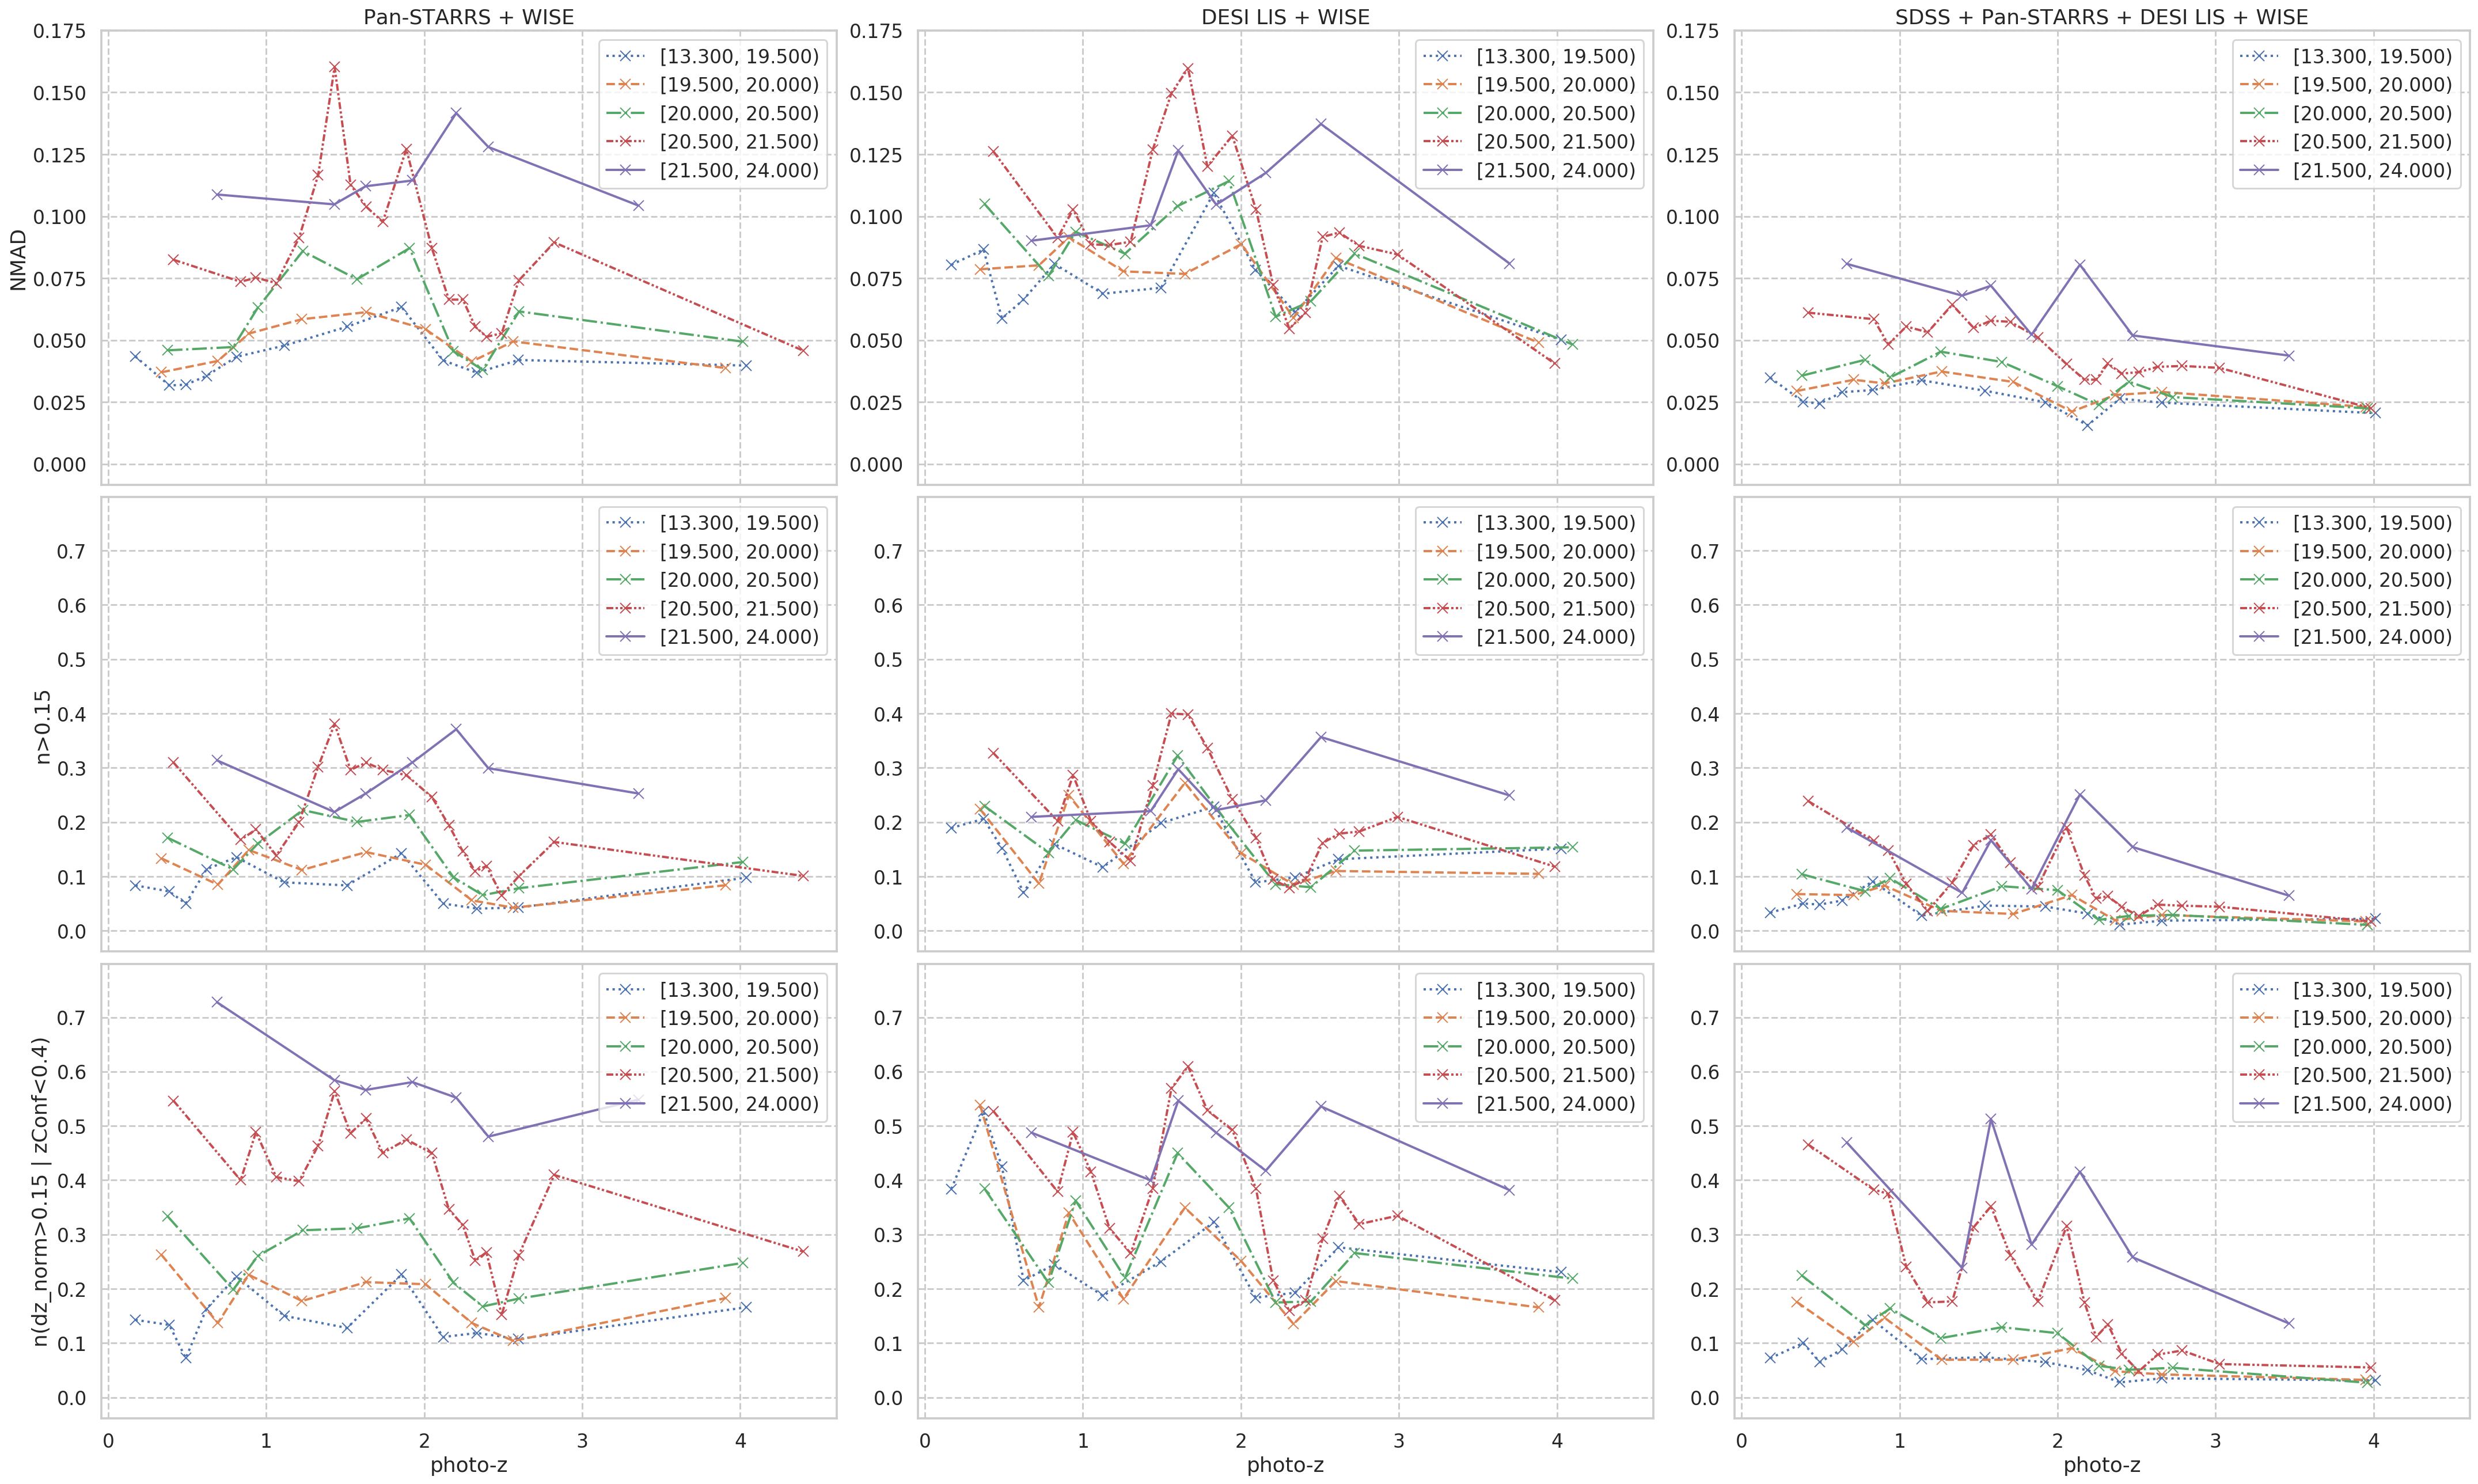
\includegraphics[width=0.9\linewidth]{images/metrics-adv-photoz-x-zmag-dr16q.png}
%    \caption{Метрики в зависимости от photo-z для разных порогов по $z_mag$ на DR16q}
%    \label{fig:my_label}
%\end{figure}
%\end{landscape}
%
%
%\begin{landscape}
%\begin{figure}
%    \centering
%    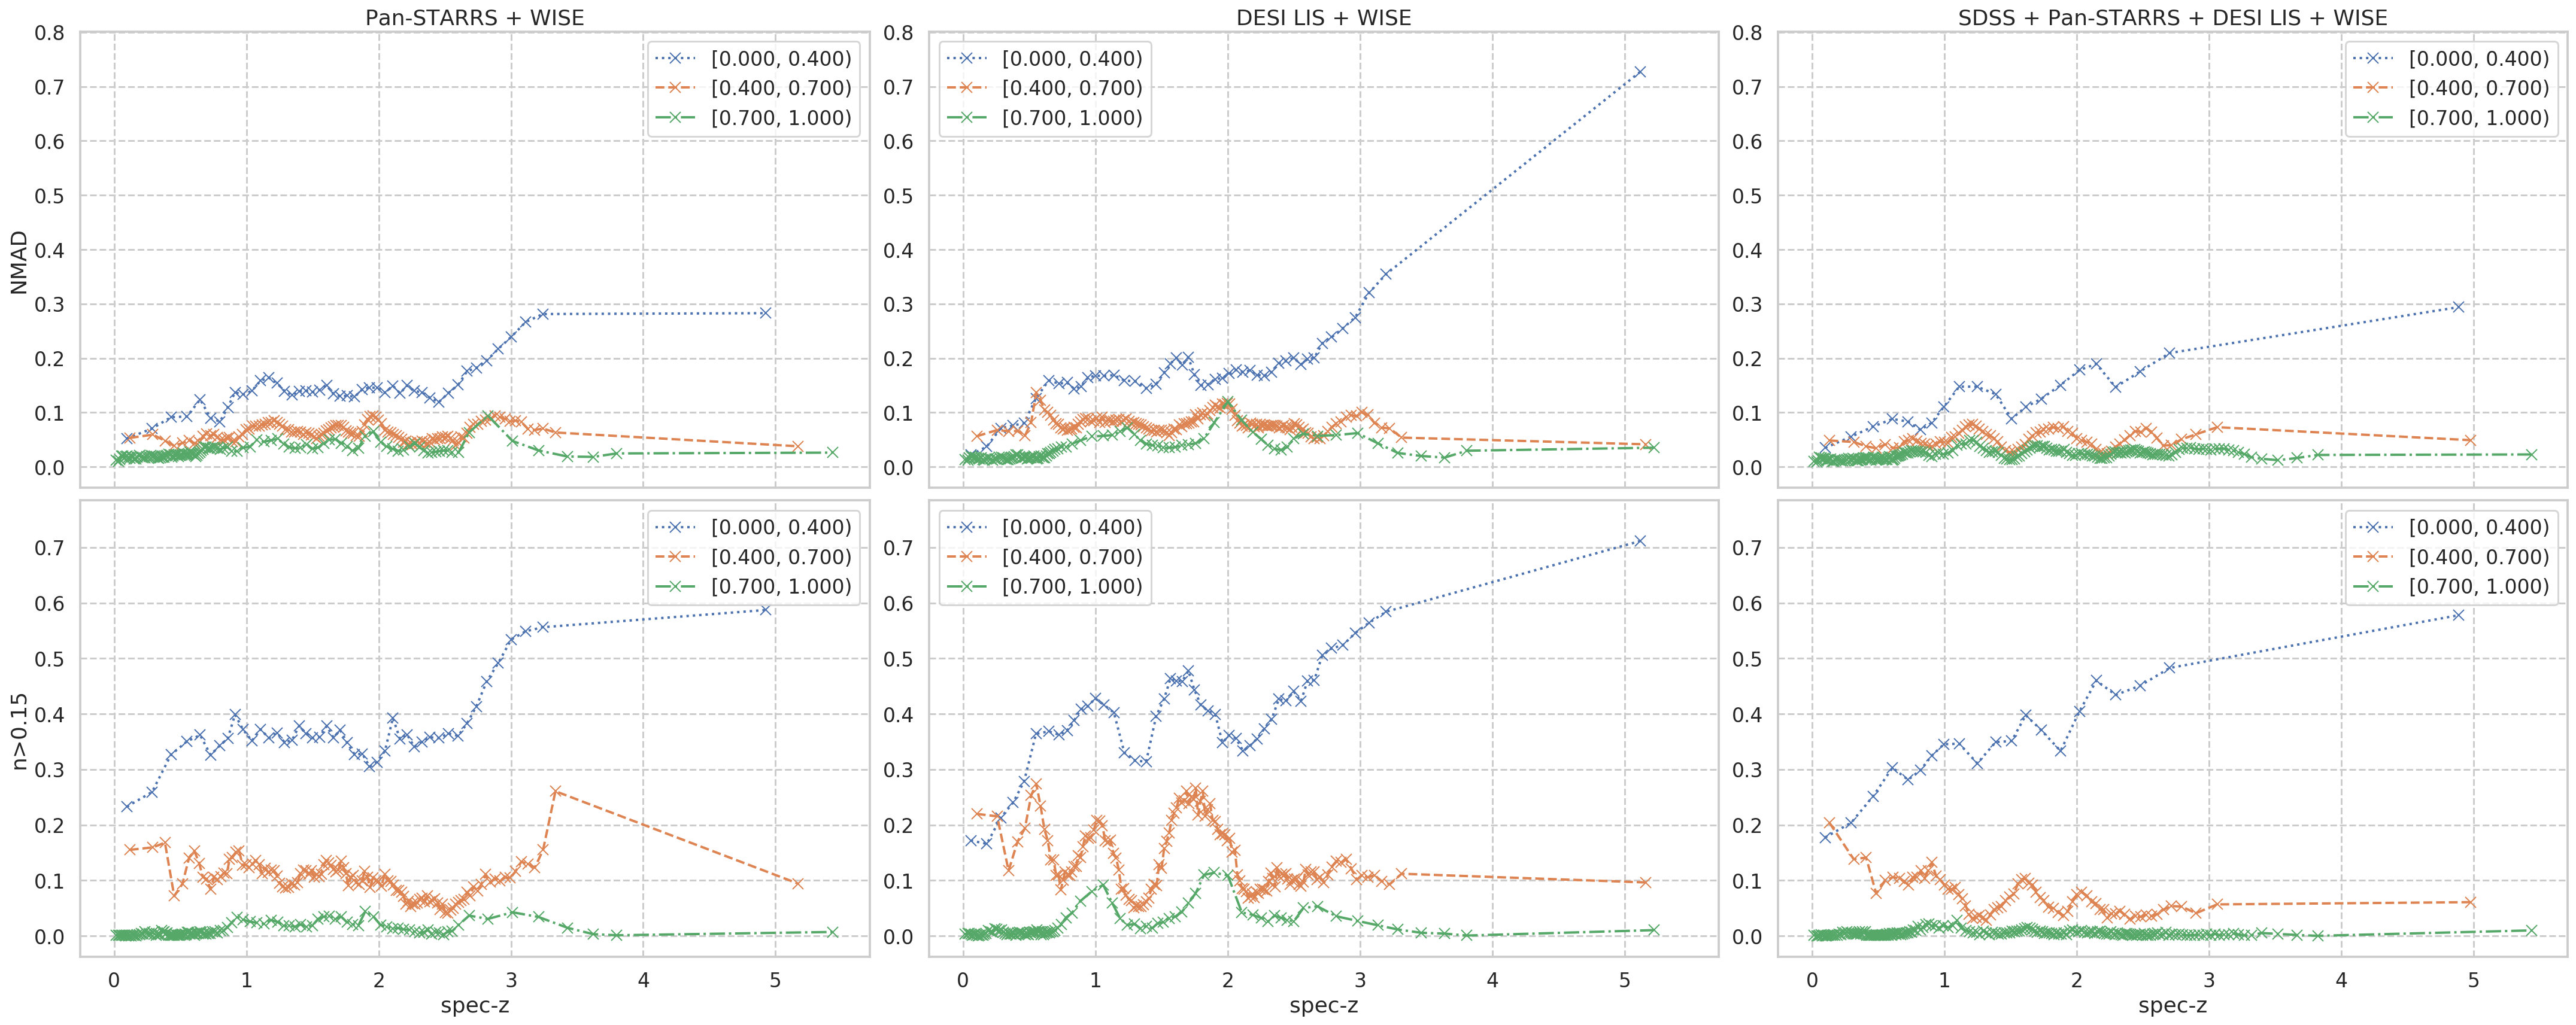
\includegraphics[width=0.9\linewidth]{images/metrics-adv-zspec-x-zconf-cv2.png}
%    \caption{Метрики в зависимости от spec-z для разных порогов по zConf на кросс-валидации}
%    \label{fig:my_label}
%\end{figure}
%\end{landscape}
%
%
%\begin{landscape}
%\begin{figure}
%    \centering
%    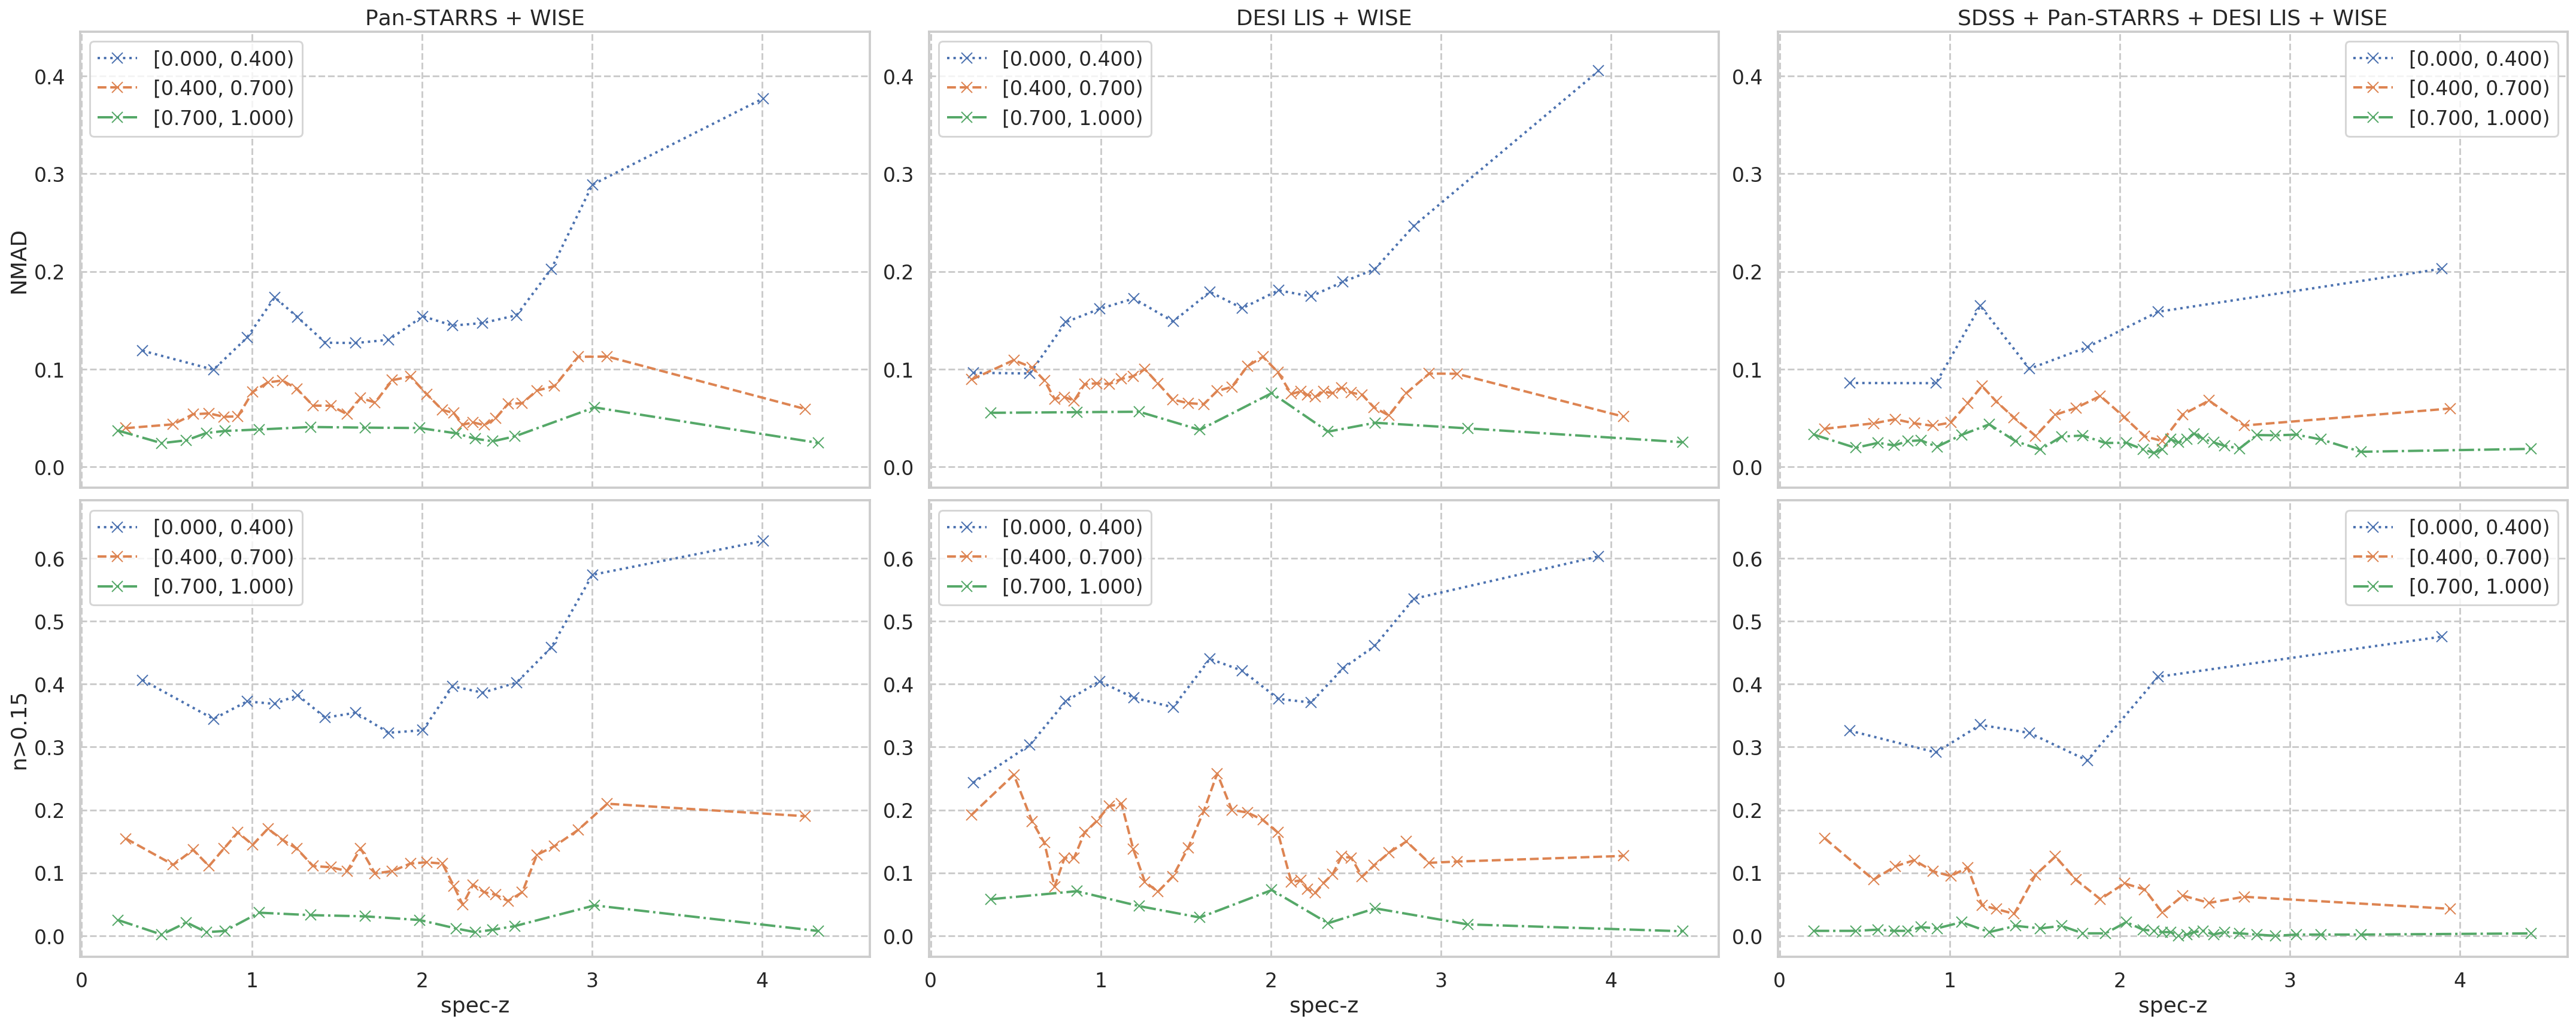
\includegraphics[width=0.9\linewidth]{images/metrics-adv-zspec-x-zconf-dr16q.png}
%    \caption{Метрики в зависимости от spec-z для разных порогов по zConf на DR16q}
%    \label{fig:my_label}
%\end{figure}
%\end{landscape}
%
%
%\begin{landscape}
%\begin{figure}
%    \centering
%    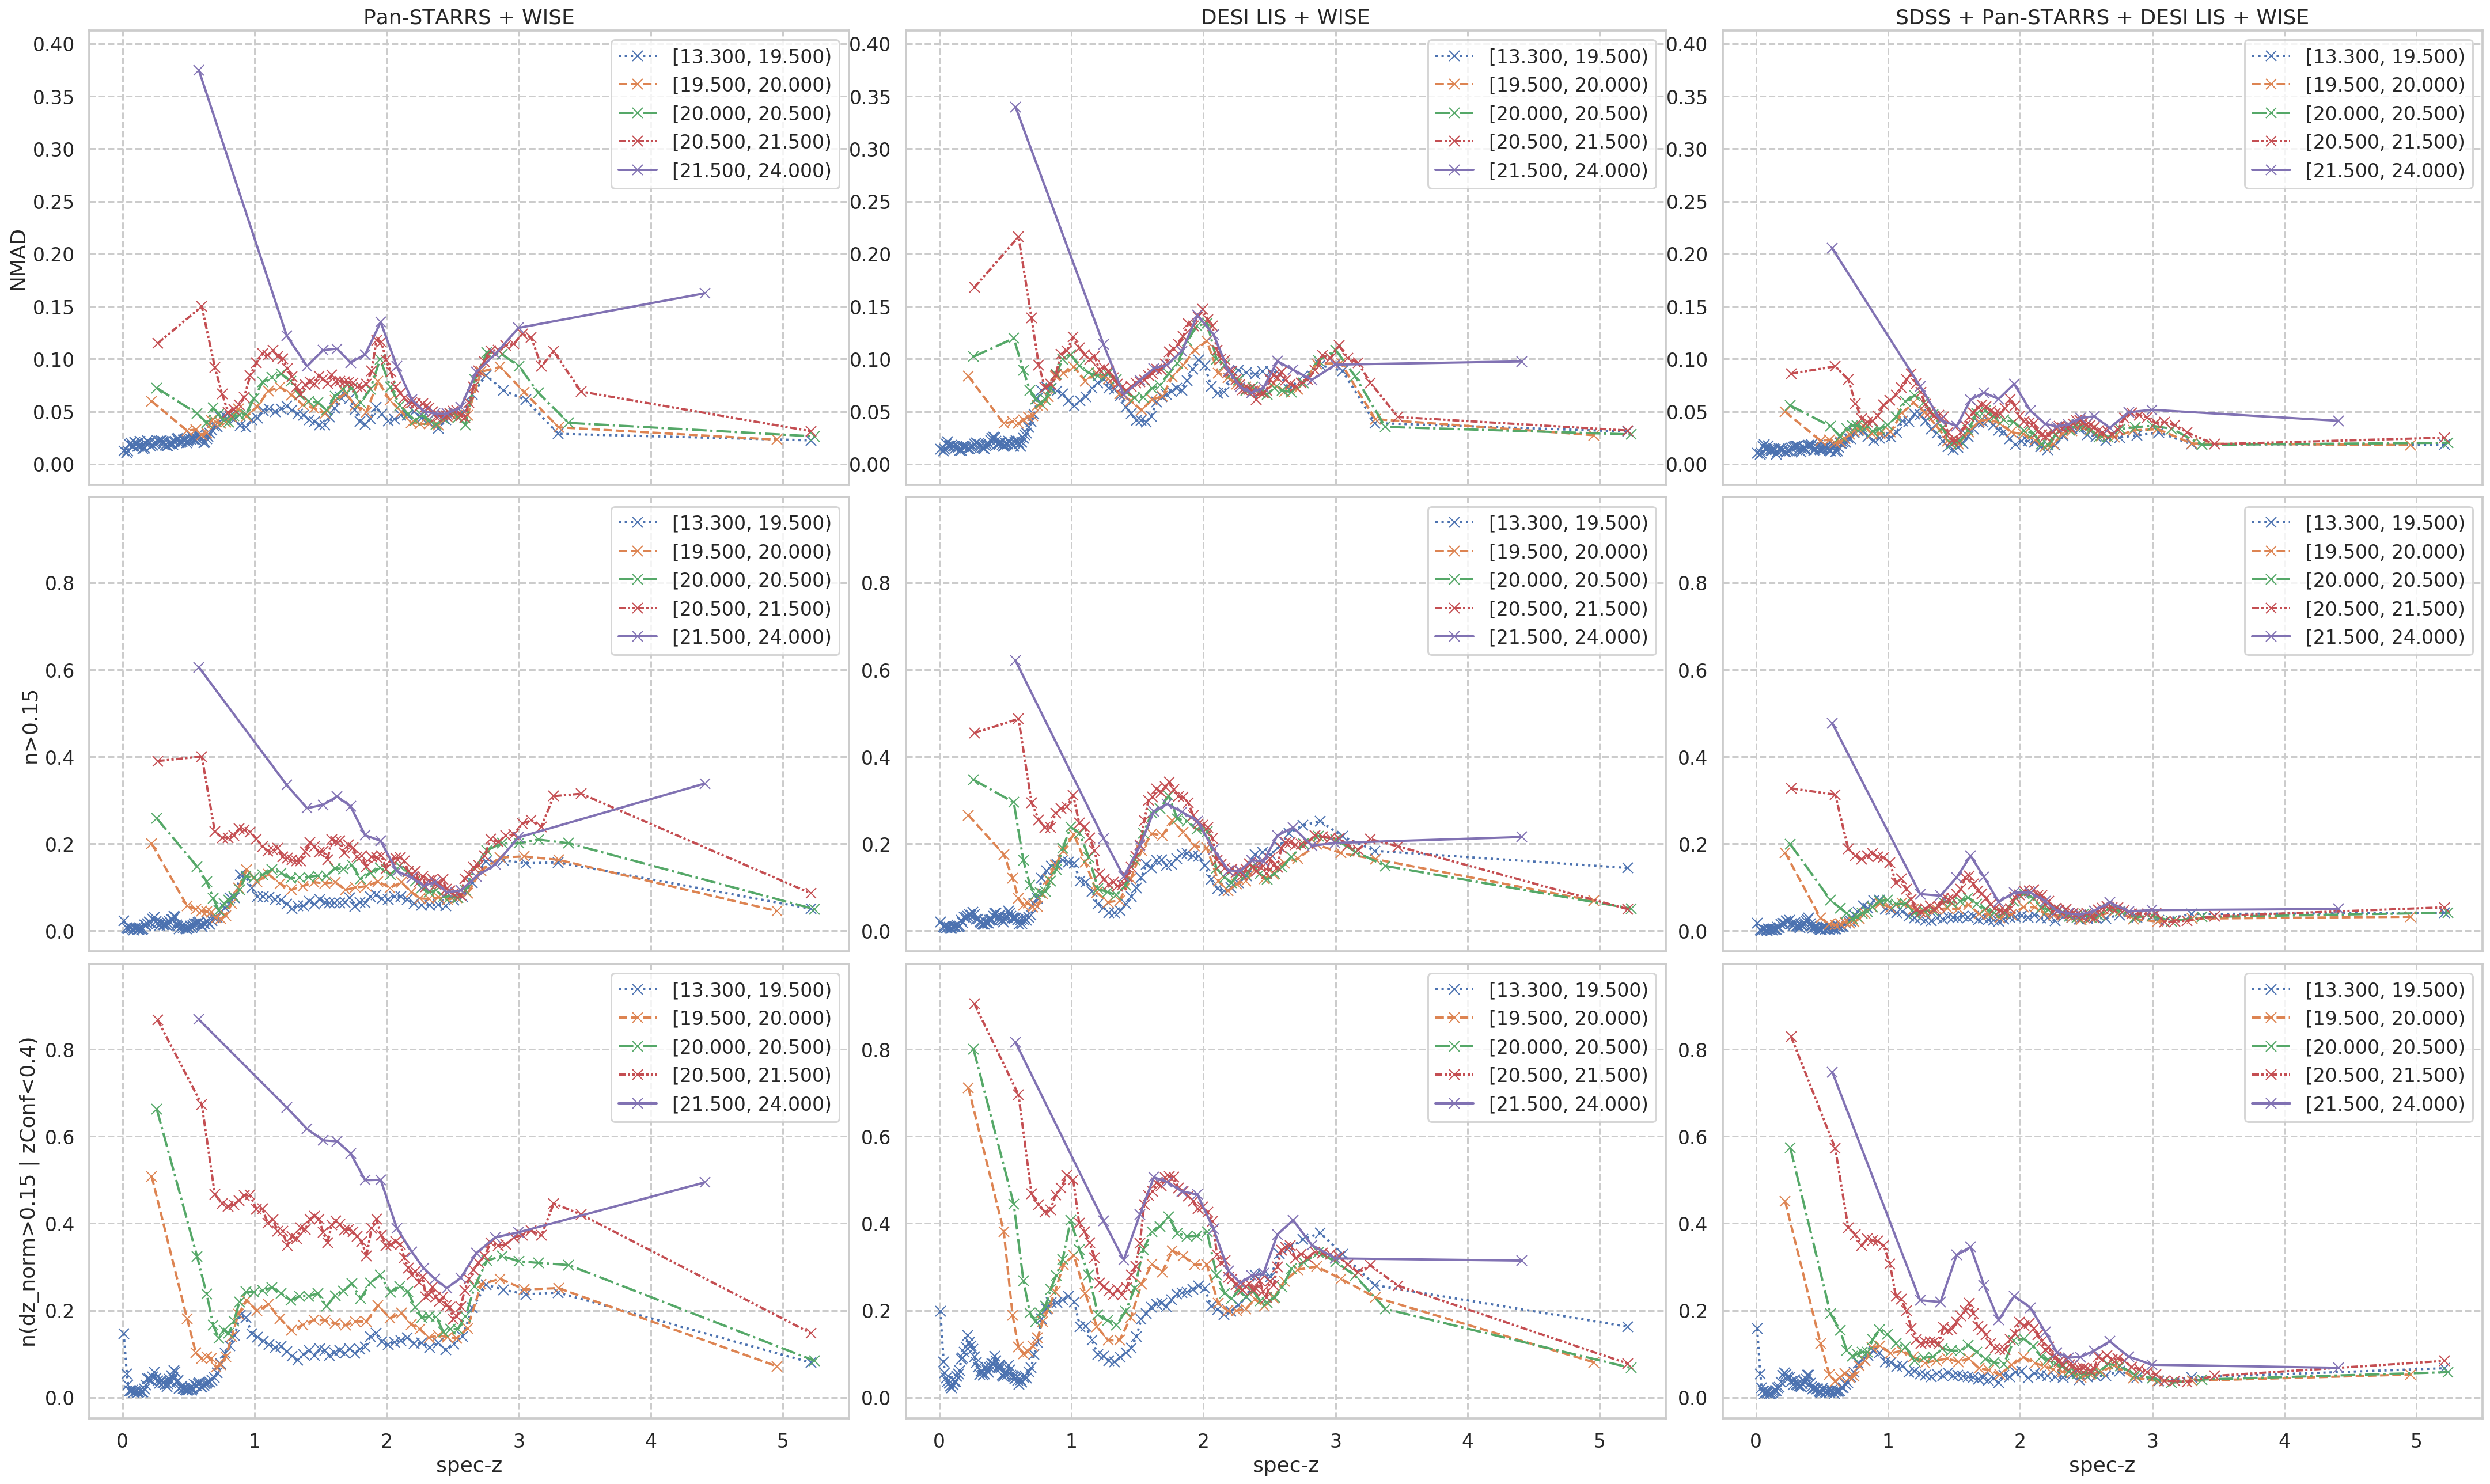
\includegraphics[width=0.9\linewidth]{images/metrics-adv-zspec-x-zmag-cv2.png}
%    \caption{Метрики в зависимости от spec-z для разных порогов по $z_mag$ на кросс-валидации}
%    \label{fig:my_label}
%\end{figure}
%\end{landscape}
%
%
%\begin{landscape}
%\begin{figure}
%    \centering
%    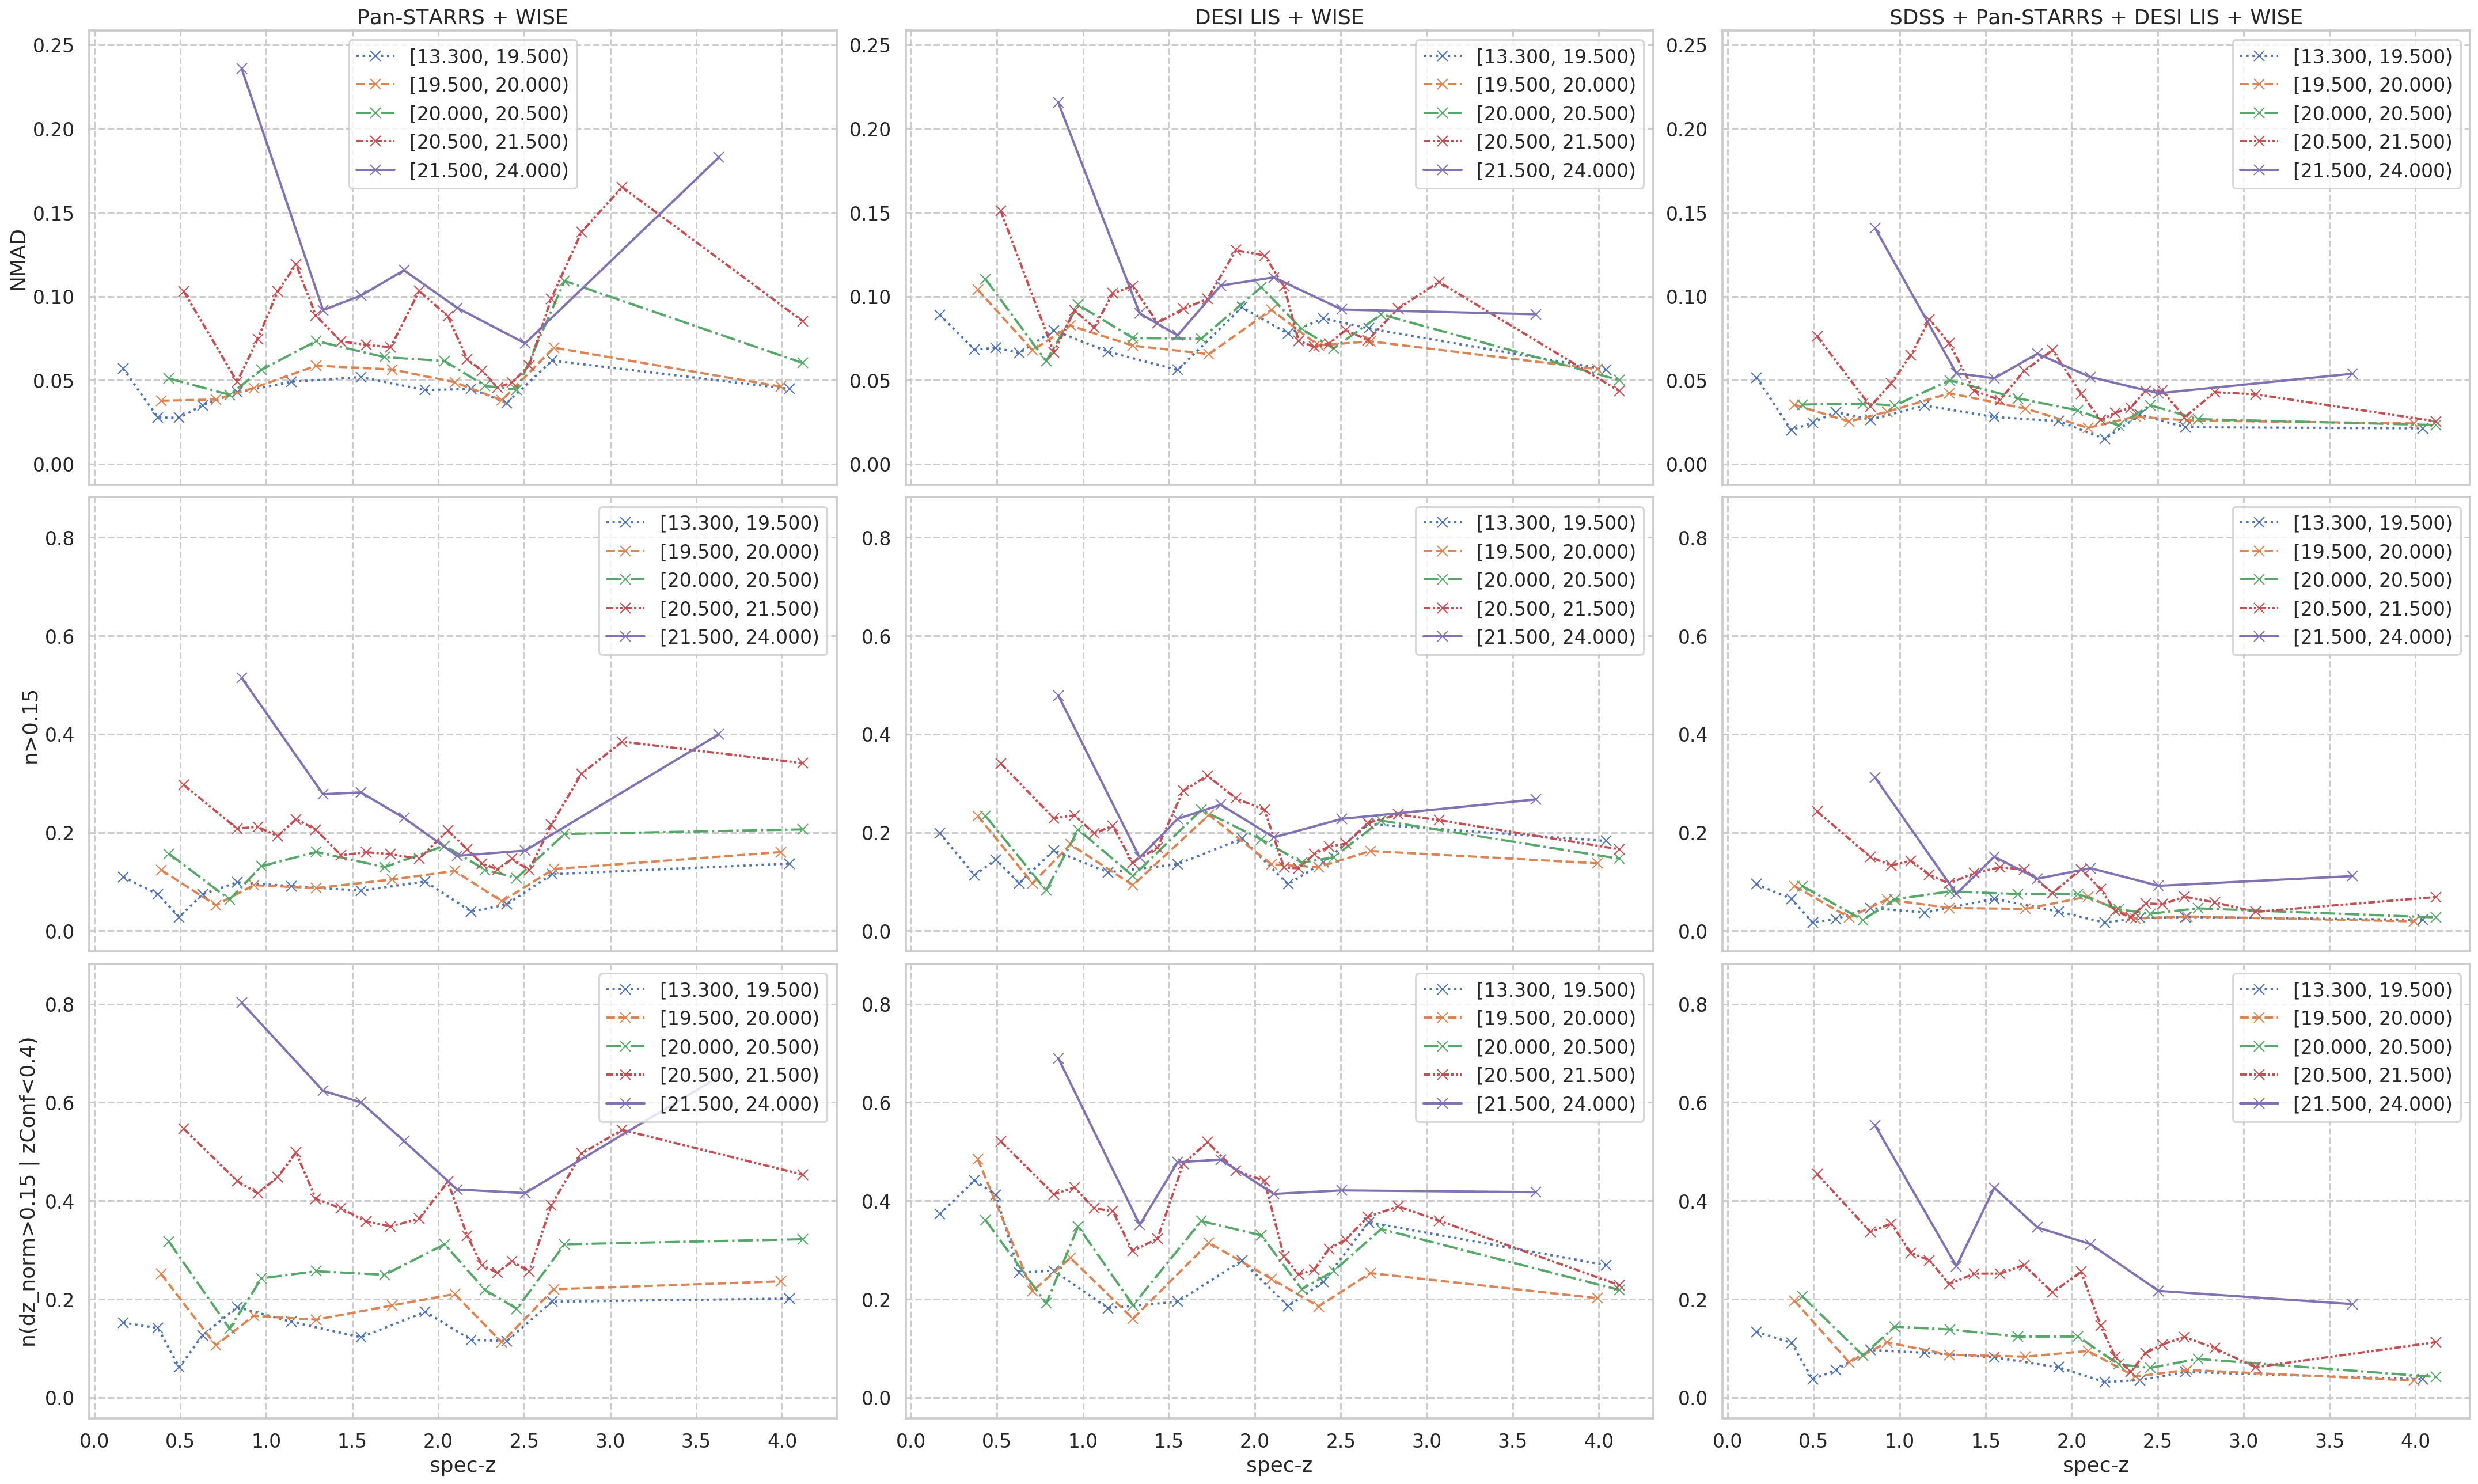
\includegraphics[width=0.9\linewidth]{images/metrics-adv-zspec-x-zmag-dr16q.png}
%    \caption{Метрики в зависимости от spec-z для разных порогов по $z_mag$ на DR16q}
%    \label{fig:my_label}
%\end{figure}
%\end{landscape}


\end{document}
